\documentclass[10pt, svgnames]{beamer}

\usetheme{Singapore}
%% \usetheme{Frankfurt}
%% \usecolortheme{seahorse}
% \usetheme{Madrid}
\setbeamertemplate{navigation symbols}{}
\setbeamertemplate{footline}[frame number]

\usepackage{etex}
\usepackage{xcolor}
\usepackage{ctable}
\usepackage{multirow}
\usepackage{tikz}
\usepackage{amsmath}
\usepackage{atlasphysics}
\usepackage{brett_latex_commands}
\usepackage[normalem]{ulem}

% ------------------------------------------------------------------------------
%% \newcommand{\Stop}{\ensuremath{\tilde{t}}}
%% \newcommand{\AntiStop}{\ensuremath{\tilde{t}^{*}}}
%% \newcommand{\TTBAR}{\ensuremath{t\bar{t}}}
%% \newcommand{\ZGAMMA}{\ensuremath{Z/\gamma^{*}}}
%% \newcommand{\Ht}{\ensuremath{H_\mathrm{T}}}
%% \newcommand{\Met}{\ensuremath{E^\mathrm{miss}_\mathrm{T}}}
%% \newcommand{\MetRel}{\ensuremath{E^\mathrm{miss,rel}_\mathrm{T}}}
%% \newcommand{\MetSig}{\ensuremath{E^\mathrm{miss}_\mathrm{T}\mathrm{ significance}}}
%% \newcommand{\MetSigEqn}{\ensuremath{E^\mathrm{miss}_\mathrm{T}/\sqrt{\Ht}}}
%% \newcommand{\Mll}{\ensuremath{m_{\ell\ell}}}
%% \newcommand{\Mbl}{\ensuremath{m_{\mathrm{b}\ell}}}
%% \newcommand{\MblAsym}{\ensuremath{m_{\mathrm{b}\ell}\mathrm{~asymmetry}}}
%% \newcommand{\MblAsymEqn}{\ensuremath{\left(\Mbl^0-\Mbl^1\right)/\left(\Mbl^0+\Mbl^1\right)}}

\colorlet{pairing_l_1}{green!50!white}
\colorlet{pairing_l_2}{green!20!white}
\colorlet{pairing_b_1}{red!50!white}
\colorlet{pairing_b_2}{red!20!white}


\colorlet{nice_blue}{RoyalBlue!80!white}
\colorlet{nice_red}{Crimson!80!white}

% ------------------------------------------------------------------------------
\newcommand{\beginbackup}{
   \newcounter{framenumbervorappendix}
   \setcounter{framenumbervorappendix}{\value{framenumber}}
}
\newcommand{\backupend}{
   \addtocounter{framenumbervorappendix}{-\value{framenumber}}
   \addtocounter{framenumber}{\value{framenumbervorappendix}} 
}

% ------------------------------------------------------------------------------
\newcommand{\Simley}[1]{%
  \begin{tikzpicture}[scale=0.11]
    \newcommand*{\SmileyRadius}{1.0}%
    \draw [fill=brown!10] (0,0) circle (\SmileyRadius)% outside circle
    %node [yshift=-0.22*\SmileyRadius cm] {\tiny #1}% uncomment this to see the smile factor
    ;

    \pgfmathsetmacro{\eyeX}{0.5*\SmileyRadius*cos(30)}
    \pgfmathsetmacro{\eyeY}{0.5*\SmileyRadius*sin(30)}
    \draw [fill=cyan,draw=none] (\eyeX,\eyeY) circle (0.15cm);
    \draw [fill=cyan,draw=none] (-\eyeX,\eyeY) circle (0.15cm);

    \pgfmathsetmacro{\xScale}{2*\eyeX/180}
    \pgfmathsetmacro{\yScale}{1.0*\eyeY}
    \draw[color=red, domain=-\eyeX:\eyeX]
    plot ({\x},{
      -0.1+#1*0.15 % shift the smiley as smile decreases
    -#1*1.75*\yScale*(sin((\x+\eyeX)/\xScale))-\eyeY});
  \end{tikzpicture}%
}%

% ------------------------------------------------------------------------------
\newcommand{\MyGrid}{
  \draw[help lines,xstep=.1,ystep=.1] (0,0) grid (1,1);
  \foreach \x in {0,1,...,9} { \node [anchor=north] at (\x/10,0) {0.\x}; }
  \foreach \y in {0,1,...,9} { \node [anchor=east] at (0,\y/10) {0.\y}; }
}


% ------------------------------------------------------------------------------
\def\tikzoverlay{%
  \tikz[baseline,overlay]\node[]
}%

\newcommand{\UpdateFlag}{
  \tikzoverlay[text width=3cm] at (10cm, +2cm) {
    \tikz node at (0., 0.) {
      \node[rectangle, rounded corners=1ex,
            minimum width=2cm, minimum height=2cm,
            fill=Goldenrod, text=black] at (0., 0.) {
        \huge
        Update slide
      };
    };
  };
}

\newcommand{\ToBackup}{
  \tikzoverlay[text width=3cm] at (10cm, +2cm) {
    \tikz node at (0., 0.) {
      \node[rectangle, rounded corners=1ex,
            minimum width=2cm, minimum height=2cm,
            fill=Goldenrod, text=black] at (0., 0.) {
        \huge
        To Backup
      };
    };
  };
}

% ------------------------------------------------------------------------------
\tikzset{
  update node/.style={
    rectangle, fill=Goldenrod, text=black, rounded corners=1ex, anchor=north east
    % draw=black,anchor=north west,
  },
}
\def\updateoverlay{%
  \tikz[baseline,overlay]\node[update node]
}%
\newcommand{\BLAH}{
  \updateoverlay[text width=3cm] at (0,0) {
    \tikz node at (0,0) {
      fml
    };
  };
}

% ------------------------------------------------------------------------------
\usetikzlibrary{decorations.pathmorphing} % foton- en gluonlijnen
\usetikzlibrary{decorations.markings} % pijltjes en dergelijke
\tikzset{
  % propagator styles
  spin0/.style={
    dashed
  },
  photon/.style={
    decorate,
    decoration={
      snake,
      amplitude=2pt,
      segment length=6pt,
      post length=0mm
    }
  },
  gluon/.style={
    decorate,
    decoration={
      coil,
      amplitude=4pt,
      segment length=8pt,
      aspect=1
    }
  },
  massvect/.style={
    decorate,
    decoration={
      snake
    }
  },
  antifermion/.style={
    postaction={
      decorate,
      decoration={
        markings,
        mark=at position .5 with {
          \draw (1.5pt,-1pt) -- (-1.5pt,0pt) -- (1.5pt,1pt);
        }
      }
    }
  },
  fermion/.style={
    postaction={
      decorate,
      decoration={
        markings,
        mark=at position .5 with {
          \draw (-1.5pt,-1pt) -- (1.5pt,0pt) -- (-1.5pt,1pt);
        }
      }
    }
  },
  toextpot/.style={
    postaction={
      decorate,
      decoration={
        markings,
        mark=at position 1 with {
          \draw (-2pt,-2pt) -- (2pt,2pt);
          \draw (-2pt,2pt) -- (2pt,-2pt);
        }
      }
    }
  },
  arclabel/.style={
    preaction={
      decorate,
      decoration={
        markings,
        mark=at position .5 with {
          \node[void] at (0,0) [label=#1]{};
        }
      }
    }
  },
  % These prevent the path from being drawn -> needs to be done twice
  momarrowr/.style={
    decorate,decoration={
      markings,
      mark=at position .5 with {
        \draw[->] (-2.5mm,-2.5mm) -- node [label=#1]{} (2.5mm,-2.5mm);
      }
    }
  },
  momarrowl/.style={
    decorate,decoration={
      markings,mark=at position .5 with {
        \draw[->] (-2.5mm,2.5mm) -- node [label=#1]{} (2.5mm,2.5mm);
      }
    }
  },
  vertex/.style={
    circle,
    draw,
    fill=black,
    inner sep=0pt,
    minimum size=.8mm
  },
  blob/.style={
    circle,
    draw=black!100,
    fill=black!15,
    inner sep=1pt,
    minimum size=5mm
  },
  void/.style={
    inner sep=0pt,
    minimum size=0pt
  },
  counterterm/.style={
    lamp,
    draw,
    inner sep=0pt,
    minimum size=6pt
  },
}


% ------------------------------------------------------------------------------
\title{
  A search for \BMINUSL\ $R$-Parity violating scalar top decays
  % in $\sqrt{s} = 8~\TeV$ pp collisions with the ATLAS experiment
}
% \subtitle{PhD Thesis Defense}
\author[Brett Jackson]{
  \textcolor{blue}{Brett Jackson}
  \\
  Evelyn Thomson
}
% \institute{University of Pennsylvania}


\AtBeginSection[]
{
  \begin{frame}{Table of Contents} \tableofcontents[currentsection]
  \end{frame}
}


\begin{document}

% ------------------------------------------------------------------------------
\begin{frame}
  \titlepage
  \centering{
    \begin{columns}
      \column{0.25\textwidth}
      \hfill
        
\includegraphics[height=0.25\textheight]{shield.pdf}
      \column{0.50\textwidth}
      \centering{
        {\color{red} PhD Thesis Defense}
      }
      \column{0.25\textwidth}
        
\includegraphics[height=0.25\textheight]{ATLAS_White_560x720_01.jpg}
    \end{columns}
  }
\end{frame}

% ==============================================================================
\section{Introduction}

% ------------------------------------------------------------------------------
\begin{frame}
  \frametitle{About me}
  \begin{description}[0ex]
    \item[2008-2010] (Philadelphia) \\
      \begin{itemize}
        \item Classes at Penn
        \item TRT timing studies
      \end{itemize}
    \item[2010-2012] (\cern) \\
      \begin{itemize}
        \item Continued work on TRT
        \item Muon isolation
        \item Small studies for $Z'$ search
      \end{itemize}
    \item[2012-2013] (\cern) \\
      \begin{itemize}
        \item Started working in SUSY group
        \item Search for direct gaugino production
      \end{itemize}
    \item[2013-2015] (\cern) \\
      \begin{itemize}
        \item \BMINUSL\ stop search (This talk)
      \end{itemize}
  \end{description}
\end{frame}

% ==============================================================================
\section{Theoretical motivation}
\subsection{Standard Model}

% ------------------------------------------------------------------------------
\begin{frame}
  \frametitle{Standard Model}
  %%
  \begin{itemize}
    \item Quantum field theory
    \item Describes matter and electroweak and strong interactions
    \item Tested over the last \textbf{50 years}!
  \end{itemize}
  %%
  \begin{center}
    \begin{tikzpicture}
      \node[
        anchor=south west,
        inner sep=0
      ] (image) at (0,0) {
        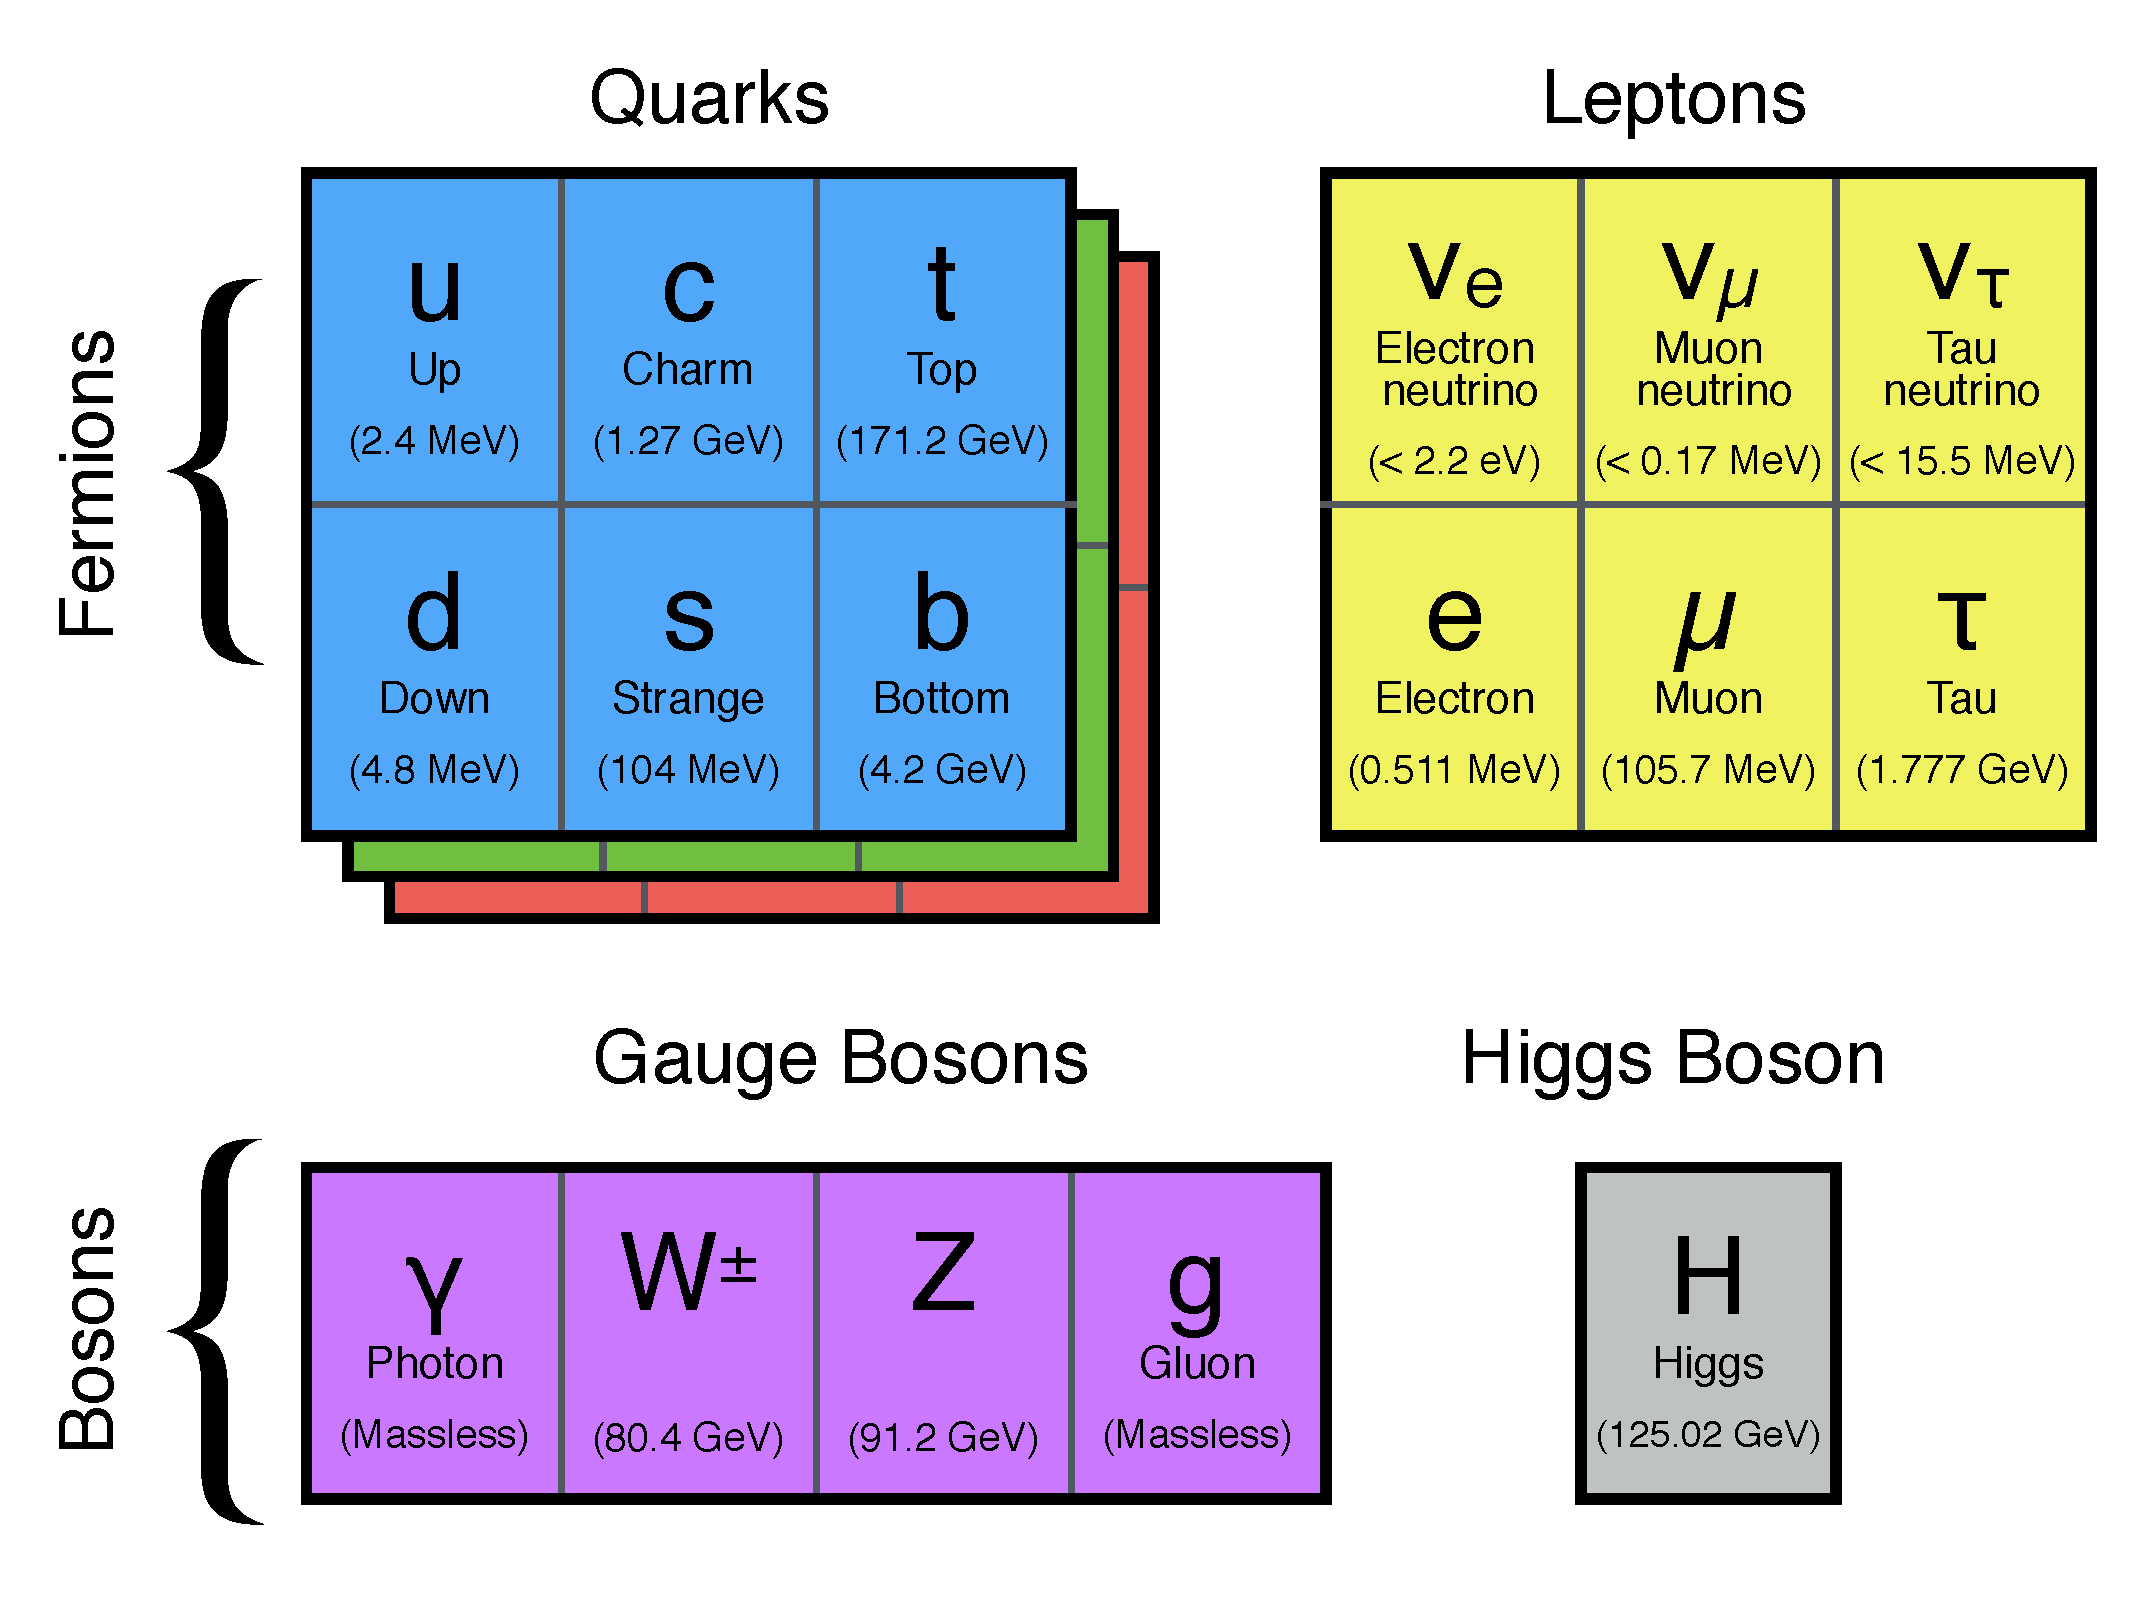
\includegraphics[width=0.65\textwidth]
        {figures/theory/sm_particle_content.pdf}
      };
      \begin{scope}[
          x={(image.south east)}, y={(image.north west)}
        ]
        %%
        \draw[
          nice_red,
          ultra thick,
          rounded corners
        ]
        (0.67, 0.02)
        rectangle
        (0.90, 0.40);
        %%
        \node[
          rectangle,
          rounded corners=1ex,
          fill=nice_blue,
          text=white,
          anchor=west
        ]
        at (0.95, 0.25) {
          \footnotesize
          \begin{tabular}{c}
            Missing until \\ 2012!
          \end{tabular}
        };
        %%
        %% \MyGrid
      \end{scope}
    \end{tikzpicture}
  \end{center}
\end{frame}

% ------------------------------------------------------------------------------
\begin{frame}
  \frametitle{Higgs boson discovery!}
  \UpdateFlag
  %%
\end{frame}

% ------------------------------------------------------------------------------
\begin{frame}
  \frametitle{Shortcomings}
  % \UpdateFlag
  %%
  \begin{columns}
    \column{0.75\textwidth}
    \begin{itemize}
      % \item \sout{Gravity not included}
      \item Gravity not included
      \item No neutrino masses with standard BEH mechanism
      \item Missing dark matter candidate
      \item Hierarchy problem
        \begin{itemize}
          \item Large difference between electroweak scale and Planck scale
          \item Radiative corrections to Higgs mass diverge quadratically
          \item Requires ``\textbf{\color{nice_blue} fine tuning}'' to obtain
            physical Higgs mass of 125~\GeV
        \end{itemize}
    \end{itemize}
    %%
    \column{0.25\textwidth}
    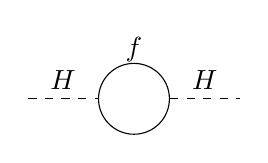
\begin{tikzpicture}[scale=0.9]
      \node[void] (in) at (0,0)  {};
      \node[void] (v1) at (1,0) {};
      \node[void] (v2) at (2,0) {};
      \node[void] (out) at (3,0) {};
      \draw[spin0] (in) -- node [above]{$H$} (v1) ;
      \draw (1.5,0) circle (0.5);
      \node at (1.5,0.7) {$f$};
      \draw[spin0] (v2) -- node [above]{$H$} (out);
    \end{tikzpicture}
    %%
    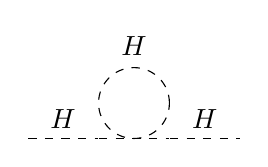
\begin{tikzpicture}[scale=0.9]
      \node[void] (in) at (0,0)  {};
      \node[void] (v1) at (1,0) {};
      \node[void] (v2) at (2,0) {};
      \node[void] (out) at (3,0) {};
      \draw[spin0] (1.5,0.5) circle (0.5);
      \node at (1.5,1.3) {$H$};
      %%
      \draw[spin0]
      (in) -- node [above]{$H$} (v1) -- (v2) -- node [above]{$H$} (out);
    \end{tikzpicture}
  \end{columns}
\end{frame}

% ==============================================================================
\subsection{Supersymmetry}

% ------------------------------------------------------------------------------
\begin{frame}
  \frametitle{Supersymmetry}
  %%
  \begin{itemize}
    \item Fermions and bosons have radiative corrections with opposite sign
    \item \textbf{\color{nice_blue} Double particle content} by introducing
      ``superpartners''
      % with different spin
      \begin{itemize}
        % \item SM fermions $\rightarrow$ boson superpartner (``sfermion'')
        % \item SM gauge bosons $\rightarrow$ fermion superpartner (``gaugino'')
        % \item Higgs doublet $\rightarrow$ Two Higgs supermultiplets +
        %   fermion superpartners (``Higgsinos'')
        \item SM fermions $\rightarrow$ boson ``sfermion''
        \item SM gauge bosons $\rightarrow$ fermion ``gaugino''
        \item Higgs doublet $\rightarrow$ Two Higgs supermultiplets +
          fermion ``Higgsinos''
      \end{itemize}
    \item Superpartners expected to have same mass as SM counterparts
    \item SUSY must be \textbf{\color{nice_blue} broken symmetry}!
  \end{itemize}
  %%
  \begin{center}
    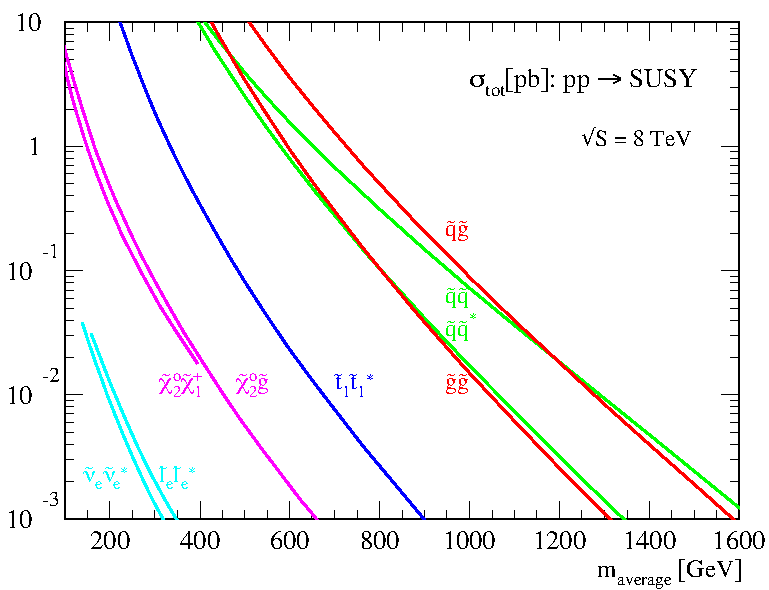
\includegraphics[width=0.5\textwidth]{figures/theory/prospino_lhc8.pdf}
  \end{center}
\end{frame}

% ------------------------------------------------------------------------------
\begin{frame}
  \frametitle{$R$-Parity}
  %%
  \begin{itemize}
    \item Generic MSSM Lagrangian violates leptons and baryon number
      \begin{itemize}
        \item 
          $W_{\Delta L = 1} =
          \frac{1}{2} \lambda^{ijk} L_{i} L_{j} \bar{e}_{k} +
          \lambda'^{ijk} L_{i} Q_{j} \bar{d}_{k} +
          \mu'^{i} L_{i} H_\mathrm{u}$
        \item 
          $W_{\Delta B = 1} =
          \frac{1}{2} \lambda''^{ijk} \bar{u}_{i} \bar{d}_{j} \bar{d}_{k}$
      \end{itemize}
    \item Lead to proton decay!
    \item Forbid these by imposing {\color{nice_blue} $R$-Parity}:
      $R=(-1)^{3(B-L)+2s}$
    \item This works, but it may be ...
  \end{itemize}
  %%
  \uncover<2->{
    \begin{center}
      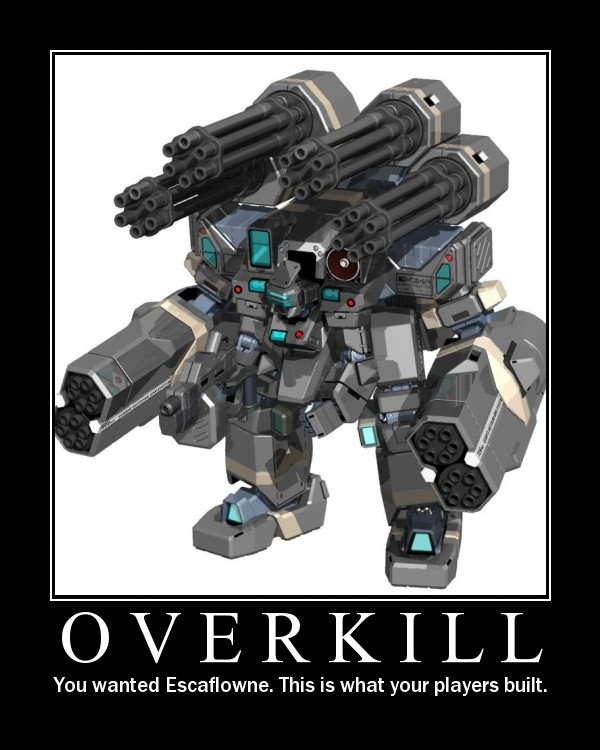
\includegraphics[
        width=0.4\textwidth,
        clip=true,
        trim=0 2.7cm 0 0
      ]
      {figures/theory/overkill.jpg}
    \end{center}
  }
  %%
\end{frame}

% ==============================================================================
\subsection{\BMINUSL\ Extension}

% ------------------------------------------------------------------------------
\begin{frame}
  \frametitle{\BMINUSL\ Extension}
  \UpdateFlag
  %%
  \begin{itemize}
    \item Introduce additional $U(1)_{B-L}$ symmetry group
    \item Anomaly arises: $\sum (\BMINUSL) = -3$
      \begin{itemize}
        \item Addition of three
          \textbf{\color{nice_blue} right-handed neutrinos} cancels anomaly
      \end{itemize}
    \item Symmetry breaking leads to vev of right-handed neutrino
    \item New term in Lagrangian:
      $W \supset
      Y_{\nu} L\,H_{u}\, \nu^{c} \to 
      Y_{\nu} \left< \tilde{\nu}^{c} \right> L\,H_{u}$
    \item Lepton number violation is allowed, but not baryon number violation
      \begin{itemize}
        \item \textbf{\color{nice_blue} No proton decay!}
      \end{itemize}
    \item (n)LSP allowed to decay
    %% \item Several choice for nLSP
    %%   \begin{itemize}
    %%     \item 
    %%   \end{itemize}
  \end{itemize}
\end{frame}

% ------------------------------------------------------------------------------
\begin{frame}
  \frametitle{(Next to) Lightest supersymmetric particle}
  \UpdateFlag
  %%
  \begin{itemize}
    \item Several natural choices for the nLSP
    \item Decays of \sbottom\ and \stau\ are more compatible with RPC searches
    \item Focus on \stop
      \begin{itemize}
        % \item \stop\ is expected to be light is most natural models
        \item {\color{nice_blue}$\stop \to b\ell$} - preferred for most of
          parameter space
        \item $\stop \to t\nu$ - negligible unless mostly ``right-handed'' \stop
      \end{itemize}
  \end{itemize}

  \vspace{1ex}

  \begin{columns}
    \column{0.50\textwidth}
    \begin{tikzpicture}
      \node[
        anchor=south west,
        inner sep=0
      ] (image) at (0,0) {
        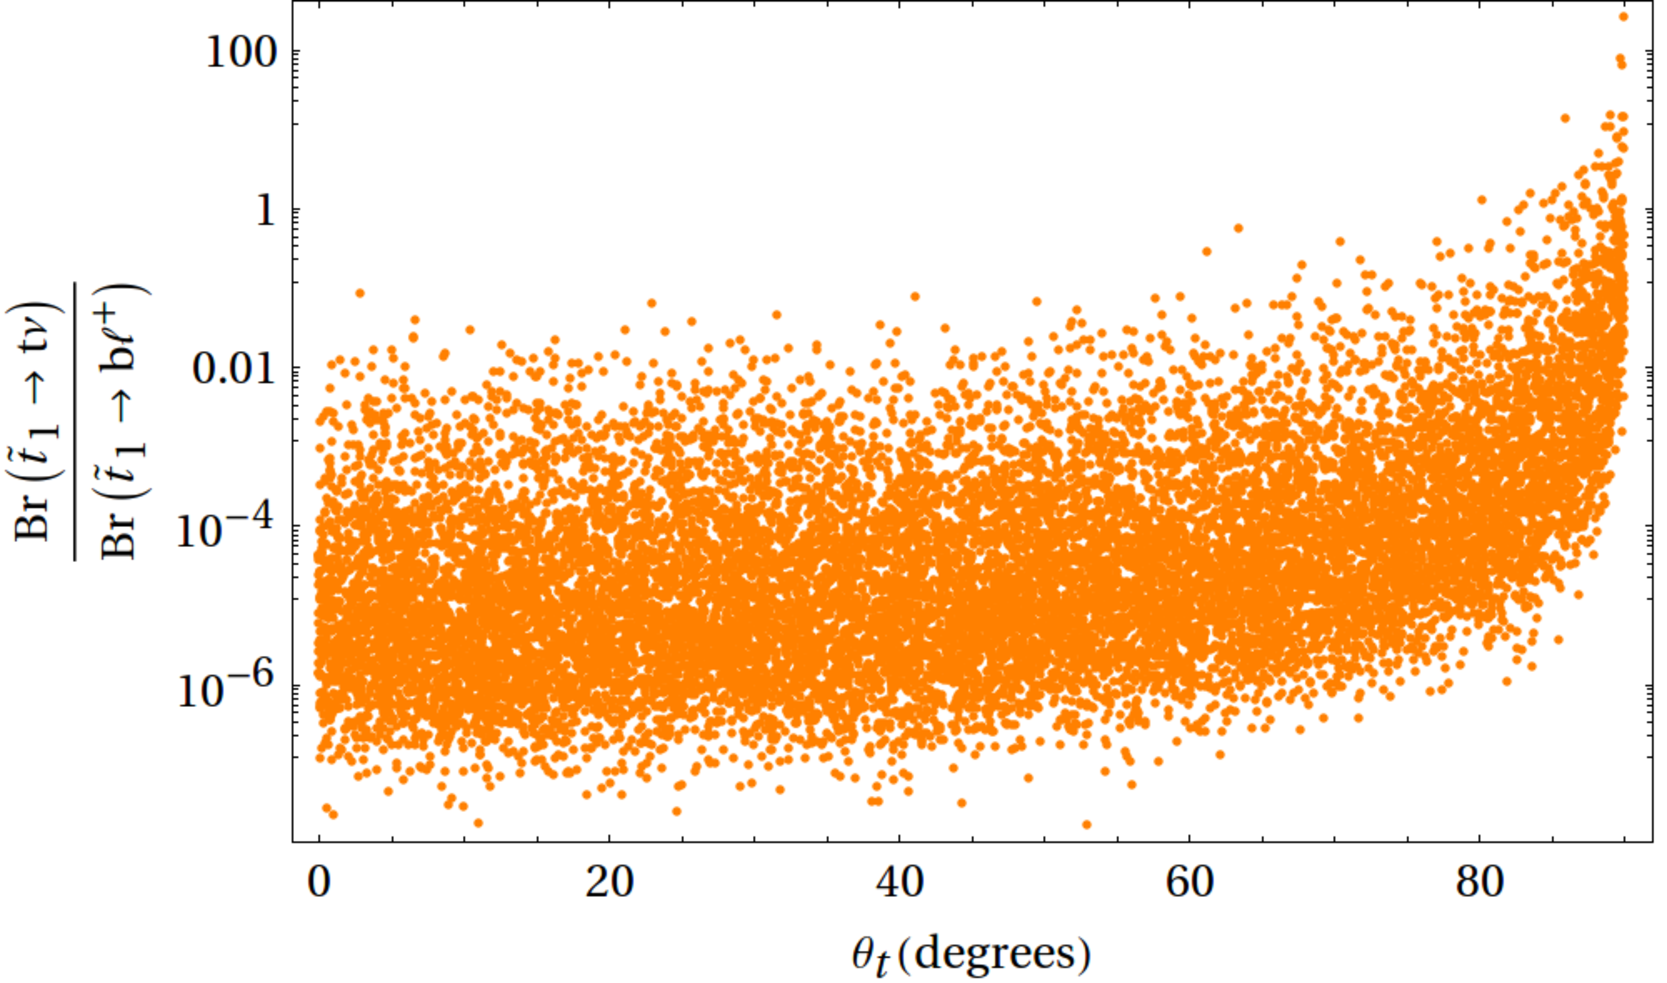
\includegraphics[width=\textwidth]
        {figures/theory/StopBranchingRatiosVsMixingAngle.pdf}
      };
      \begin{scope}[
          x={(image.south east)}, y={(image.north west)}
        ]
        %%
        \draw[black, thick] (0.18, 0.80) -- (0.98, 0.80);
        %%
        % \MyGrid
      \end{scope}
    \end{tikzpicture}
    \column{0.50\textwidth}
      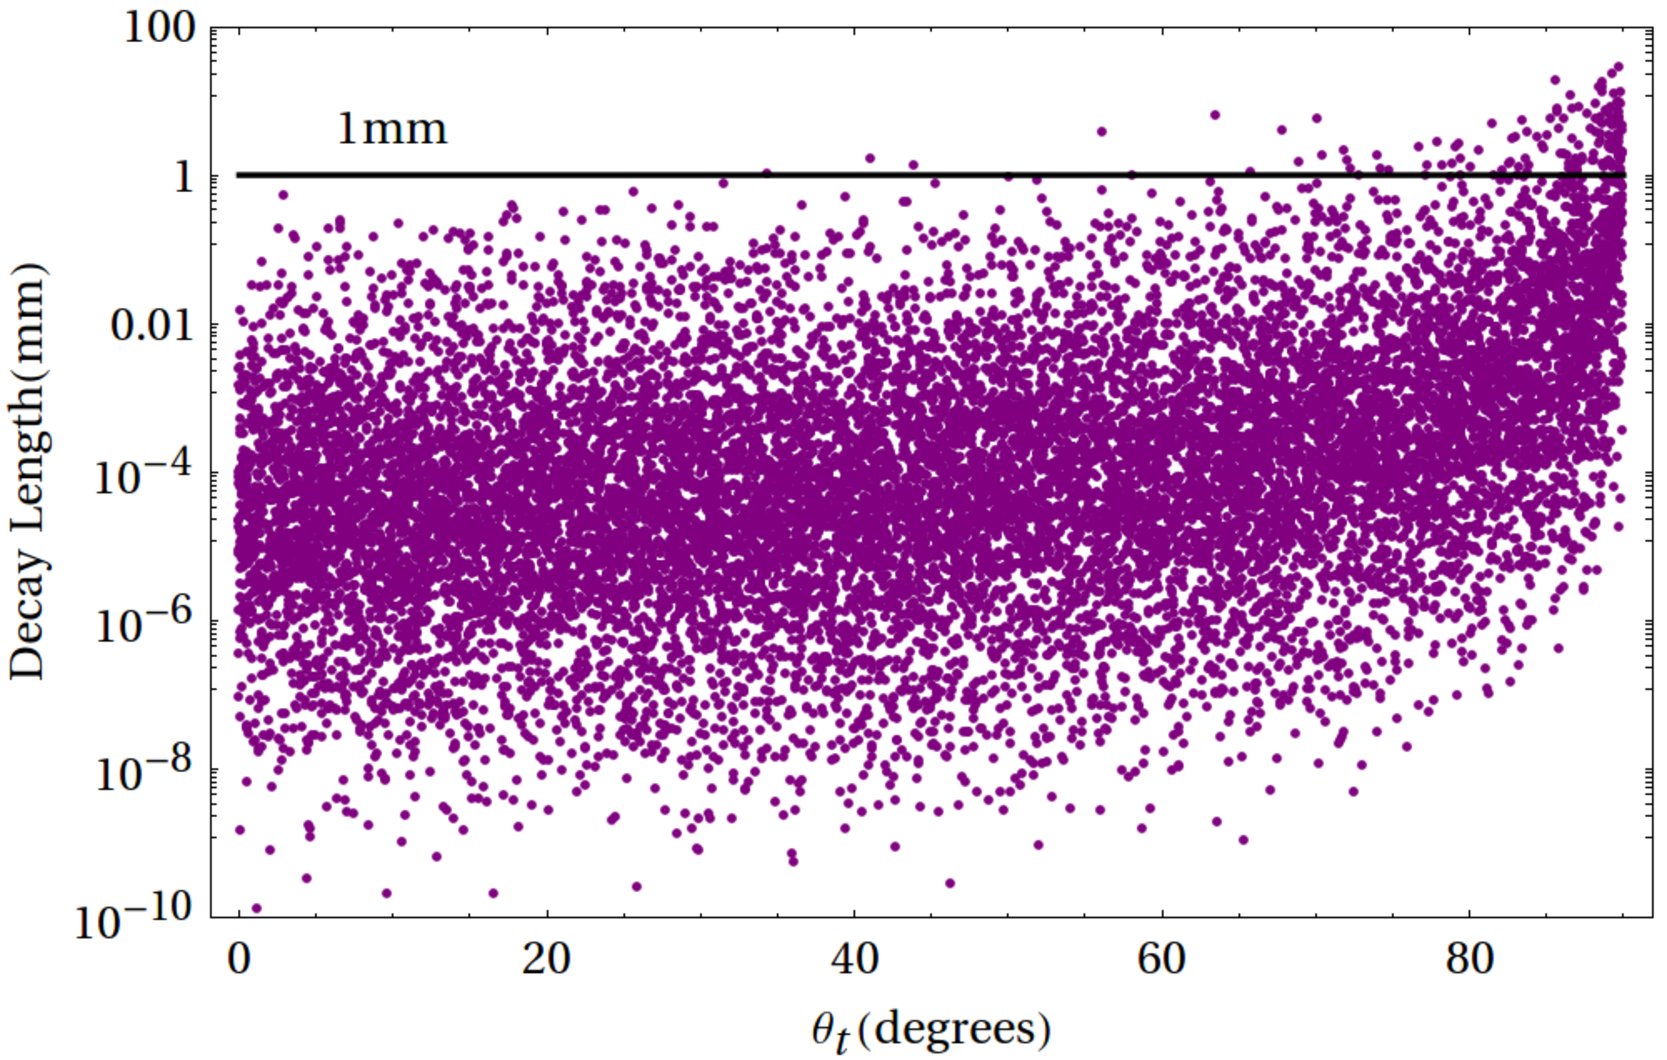
\includegraphics[width=\textwidth]{figures/theory/DecayLength.pdf}
    \end{columns}
\end{frame}

%% % ------------------------------------------------------------------------------
\begin{frame}
  \frametitle{\BMINUSL\ \stop\ decays}
  %%
  \begin{center}
    \begin{tikzpicture}
      \node[
        anchor=south west,
        inner sep=0
      ] (image) at (0,0) {
        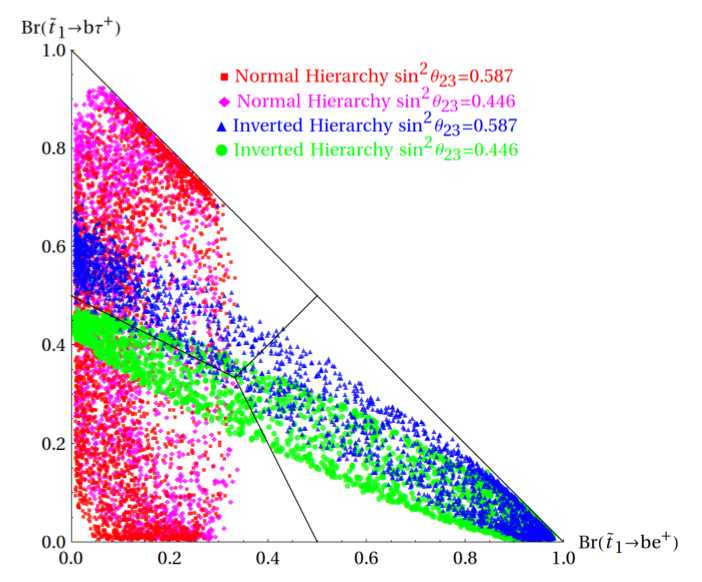
\includegraphics[width=0.5\linewidth]{figures/stop_model_scan.png}
      };
      \begin{scope}[x={(image.south east)}, y={(image.north west)}]
        \node[rectangle,
          rounded corners=1ex,
          fill=RoyalBlue!30!white
        ] at (0.65, 0.95) {
          \scriptsize
          \href{http://arxiv.org/abs/1402.5434}{arxiv:1402.5434}
        };
        \node[
          rectangle,
          rounded corners=1ex,
          fill=RoyalBlue!80!white,
          text=white
        ] at (0.95, 0.2) {
          Mostly $ee$
        };
        \node[
          rectangle,
          rounded corners=1ex,
          fill=RoyalBlue!80!white,
          text=white
        ] at (-0.15, 0.2) {
          Mostly $\mu\mu$
        };
        \node[
          rectangle,
          rounded corners=1ex,
          fill=ForestGreen!80!white,
          text=white
        ] at (0.85, 0.5) {
          \footnotesize
          \begin{tabular}{c}
            Branching ratios of \\
            $\tilde{t}\rightarrow b\ell$ related to \\
            neutrino hierarchy
          \end{tabular}
        };
        %%
        % \MyGrid
        %%
        \end{scope}
      \end{tikzpicture}
  \end{center}
  %%
  \begin{itemize}
    \item Decay of the nLSP is related to the neutrino sector
    \item Differs from traditional leptoquark searches because decay can
      include $b$-quark and a \textbf{\color{nice_blue} light lepton}
  \end{itemize}
  %%
\end{frame}
% ------------------------------------------------------------------------------
\begin{frame}
  \frametitle{Previous results}
  %%
  \begin{itemize}
    \item Previously, \textbf{\color{nice_blue}no direct search} for this model
    \item Results from leptoquark searches have been reinterpreted
    \item Goal of this analysis is to
      % discover new particle \Simley{0.5} or
      % improve this limit \Simley{-0.5}
      \begin{itemize}
        \item discover new particle \Simley{0.5}
        \item or, improve this limit \Simley{-0.5}
      \end{itemize}
  \end{itemize}
  %%
  \begin{center}
    \begin{tikzpicture}
      \node[anchor=south west, inner sep=0] (image) at (0,0) {
        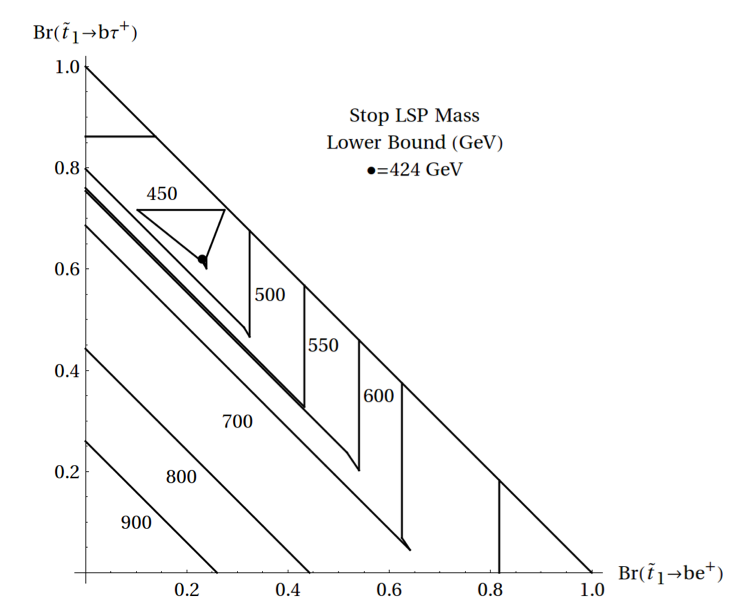
\includegraphics[width=0.6\textwidth]{figures/pheno_limit.png}
      };
      \begin{scope}[
          x={(image.south east)},
          y={(image.north west)}
        ]
        \node[
          rectangle,
          rounded corners=1ex,
          fill=RoyalBlue!30!white
        ]
        at (0.65, 0.95) {
          \scriptsize
          \href{http://arxiv.org/abs/1402.5434}{arxiv:1402.5434}
        };
        %%
        % \MyGrid
      \end{scope}
    \end{tikzpicture}
  \end{center}
  %%
\end{frame}

% ==============================================================================
\section{Experimental apparatus}
\subsection{LHC}

% ------------------------------------------------------------------------------
\begin{frame}
  \frametitle{LHC}
  %%
  \begin{center}
    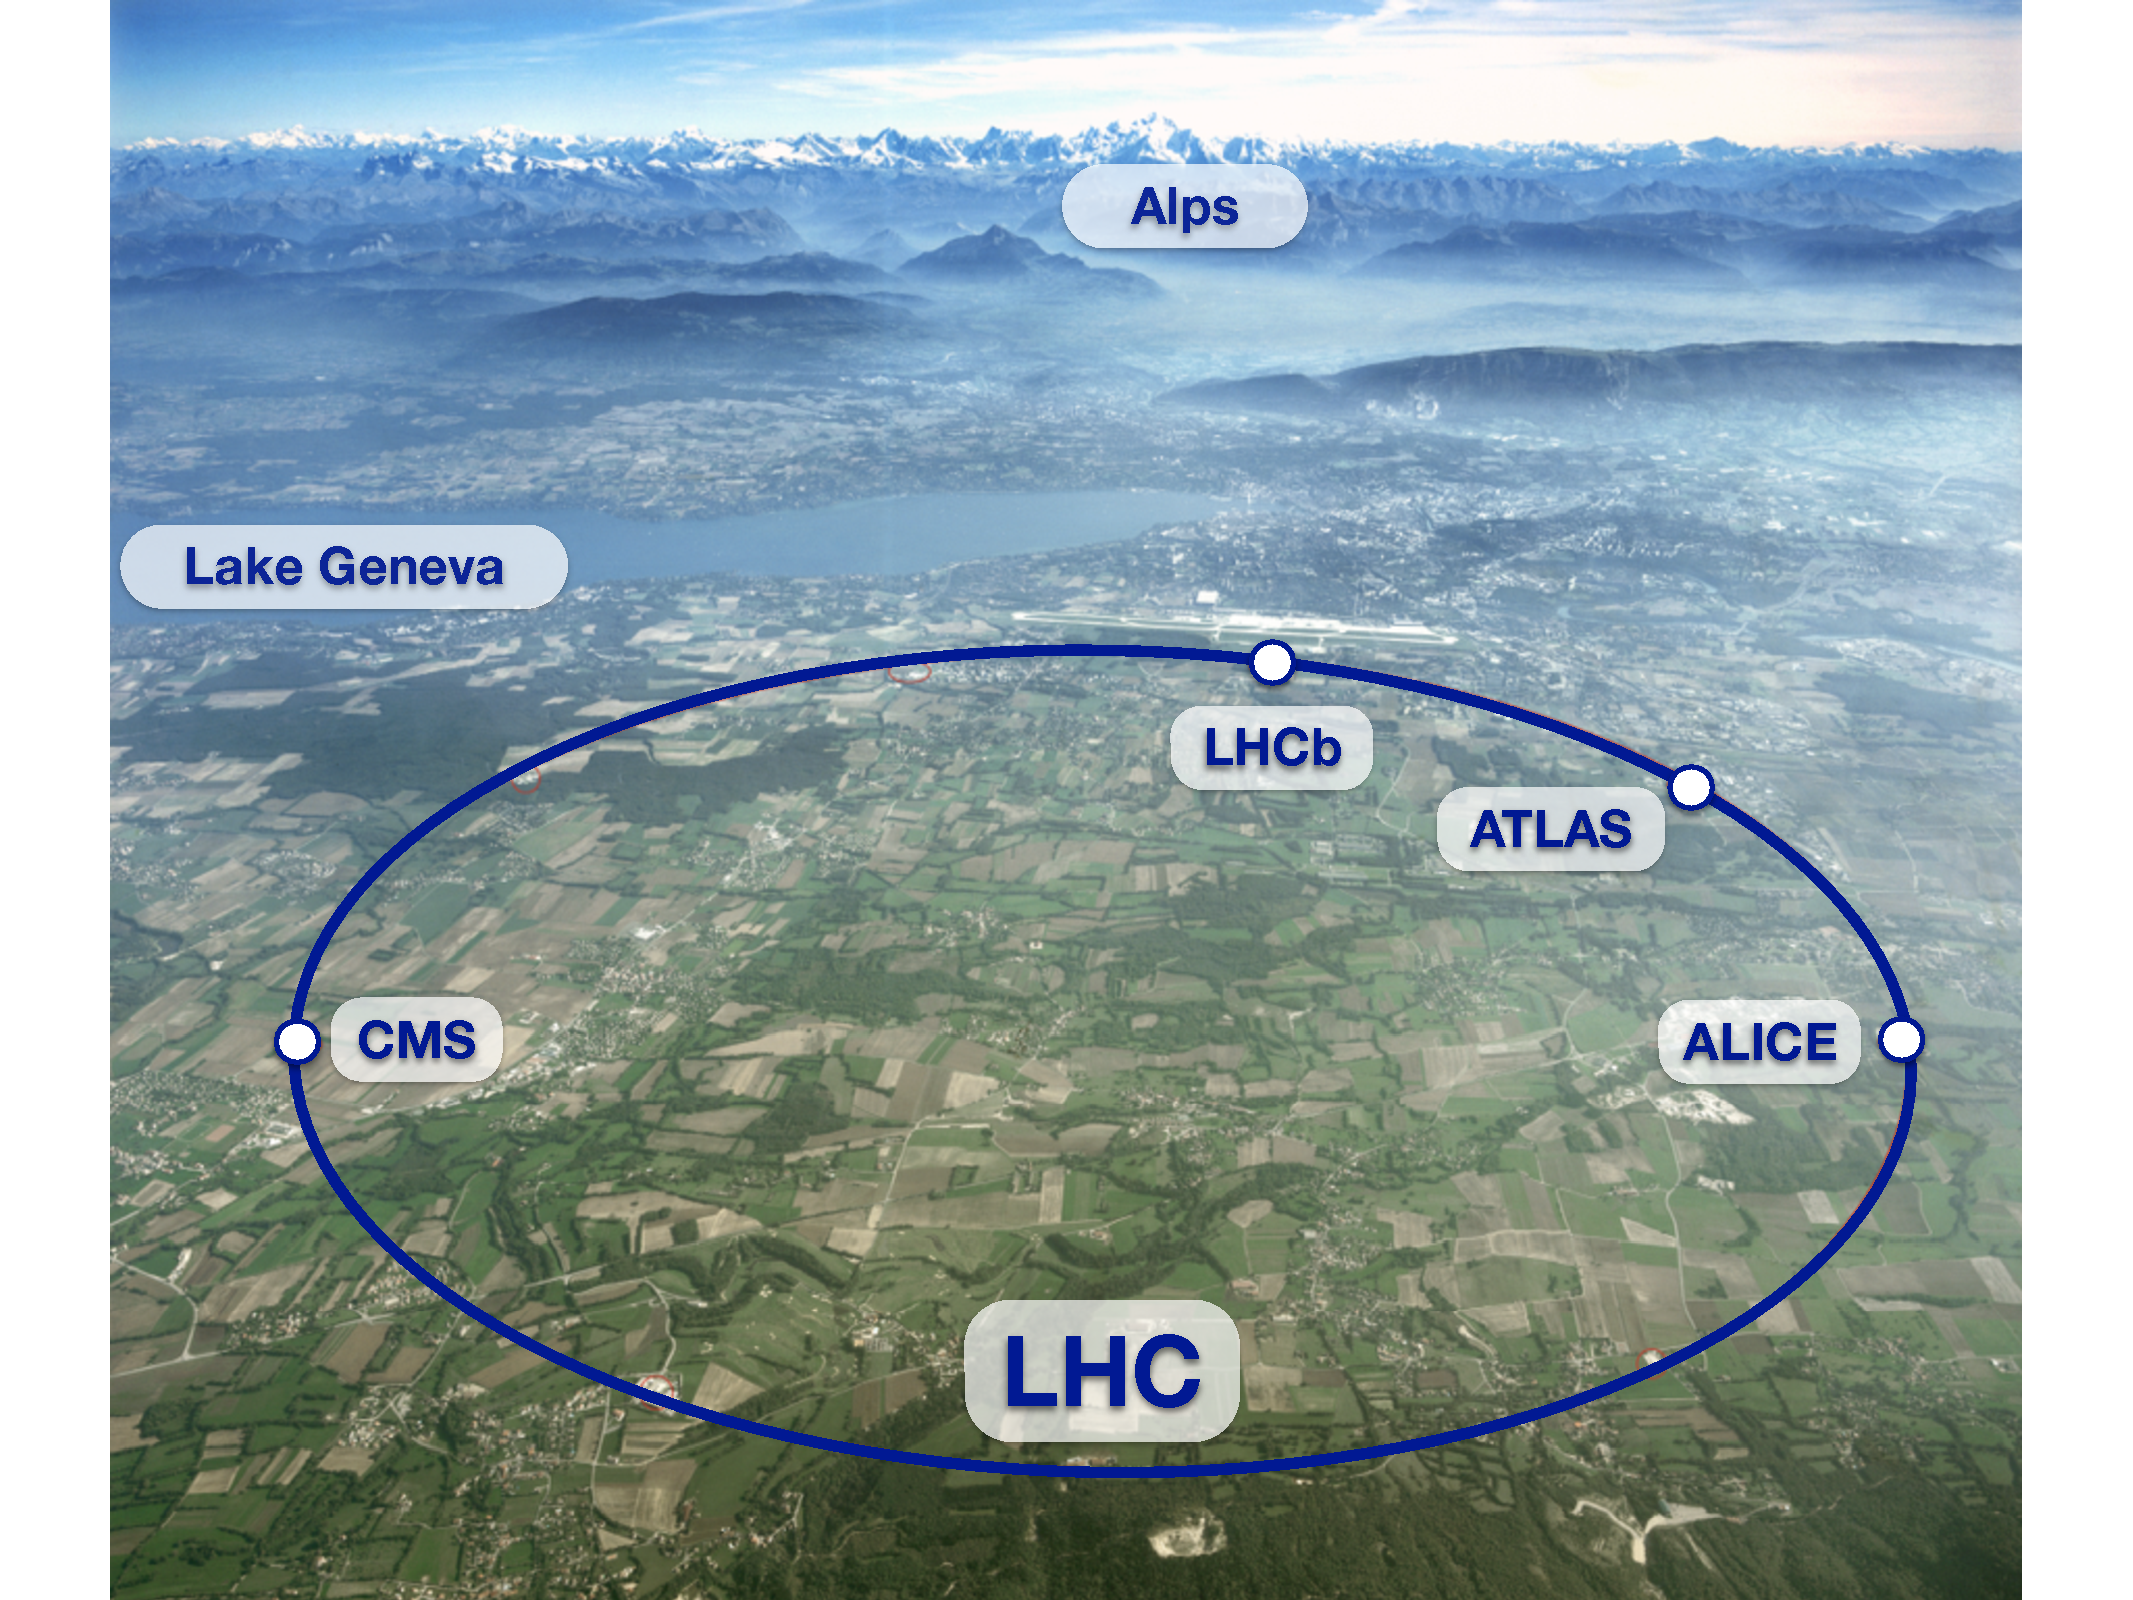
\includegraphics[width=0.95\textwidth]
    {figures/lhc_and_atlas/lhc_aerial.pdf}
  \end{center}
\end{frame}

% ------------------------------------------------------------------------------
\begin{frame}
  \frametitle{LHC}
  %%
  \begin{itemize}
    \item 27~km in circumference
    \item 8~\TeV\ center-of-mass energy
    \item 20.3~\ifb\ of $pp$ collision data in 2012
  \end{itemize}
  %%
  \begin{center}
    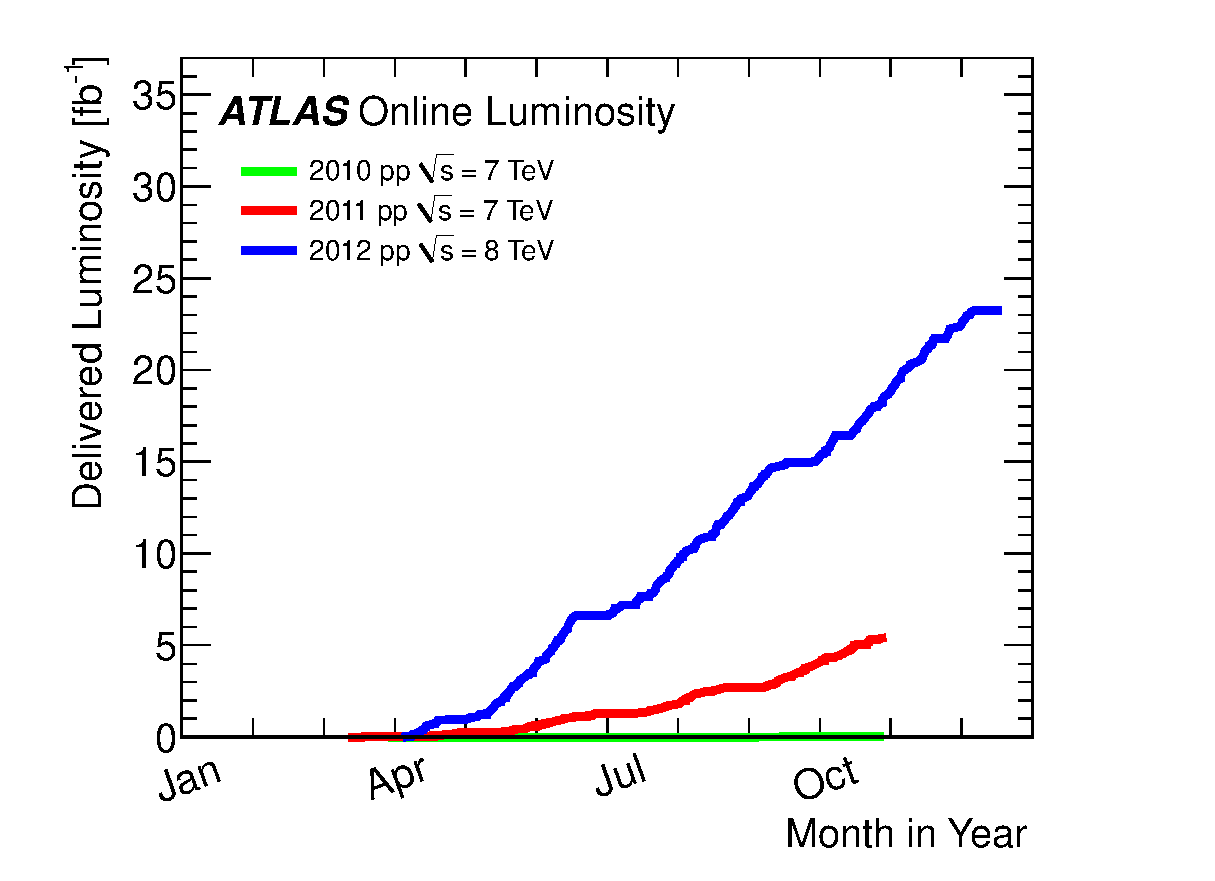
\includegraphics[width=0.8\textwidth]
    {figures/lhc_and_atlas/intlumivsyear.eps}
  \end{center}
\end{frame}

% ==============================================================================
\subsection{The \atlas\ experiment}

% ------------------------------------------------------------------------------
\begin{frame}
  \frametitle{\atlas}
  %%
  \begin{center}
    \includegraphics[width=\textwidth]
    {figures/lhc_and_atlas/atlas_det_dino_1.jpg}
  \end{center}
\end{frame}

% ------------------------------------------------------------------------------
\begin{frame}
  \frametitle{Particle signatures}
  %%
  \begin{center}
    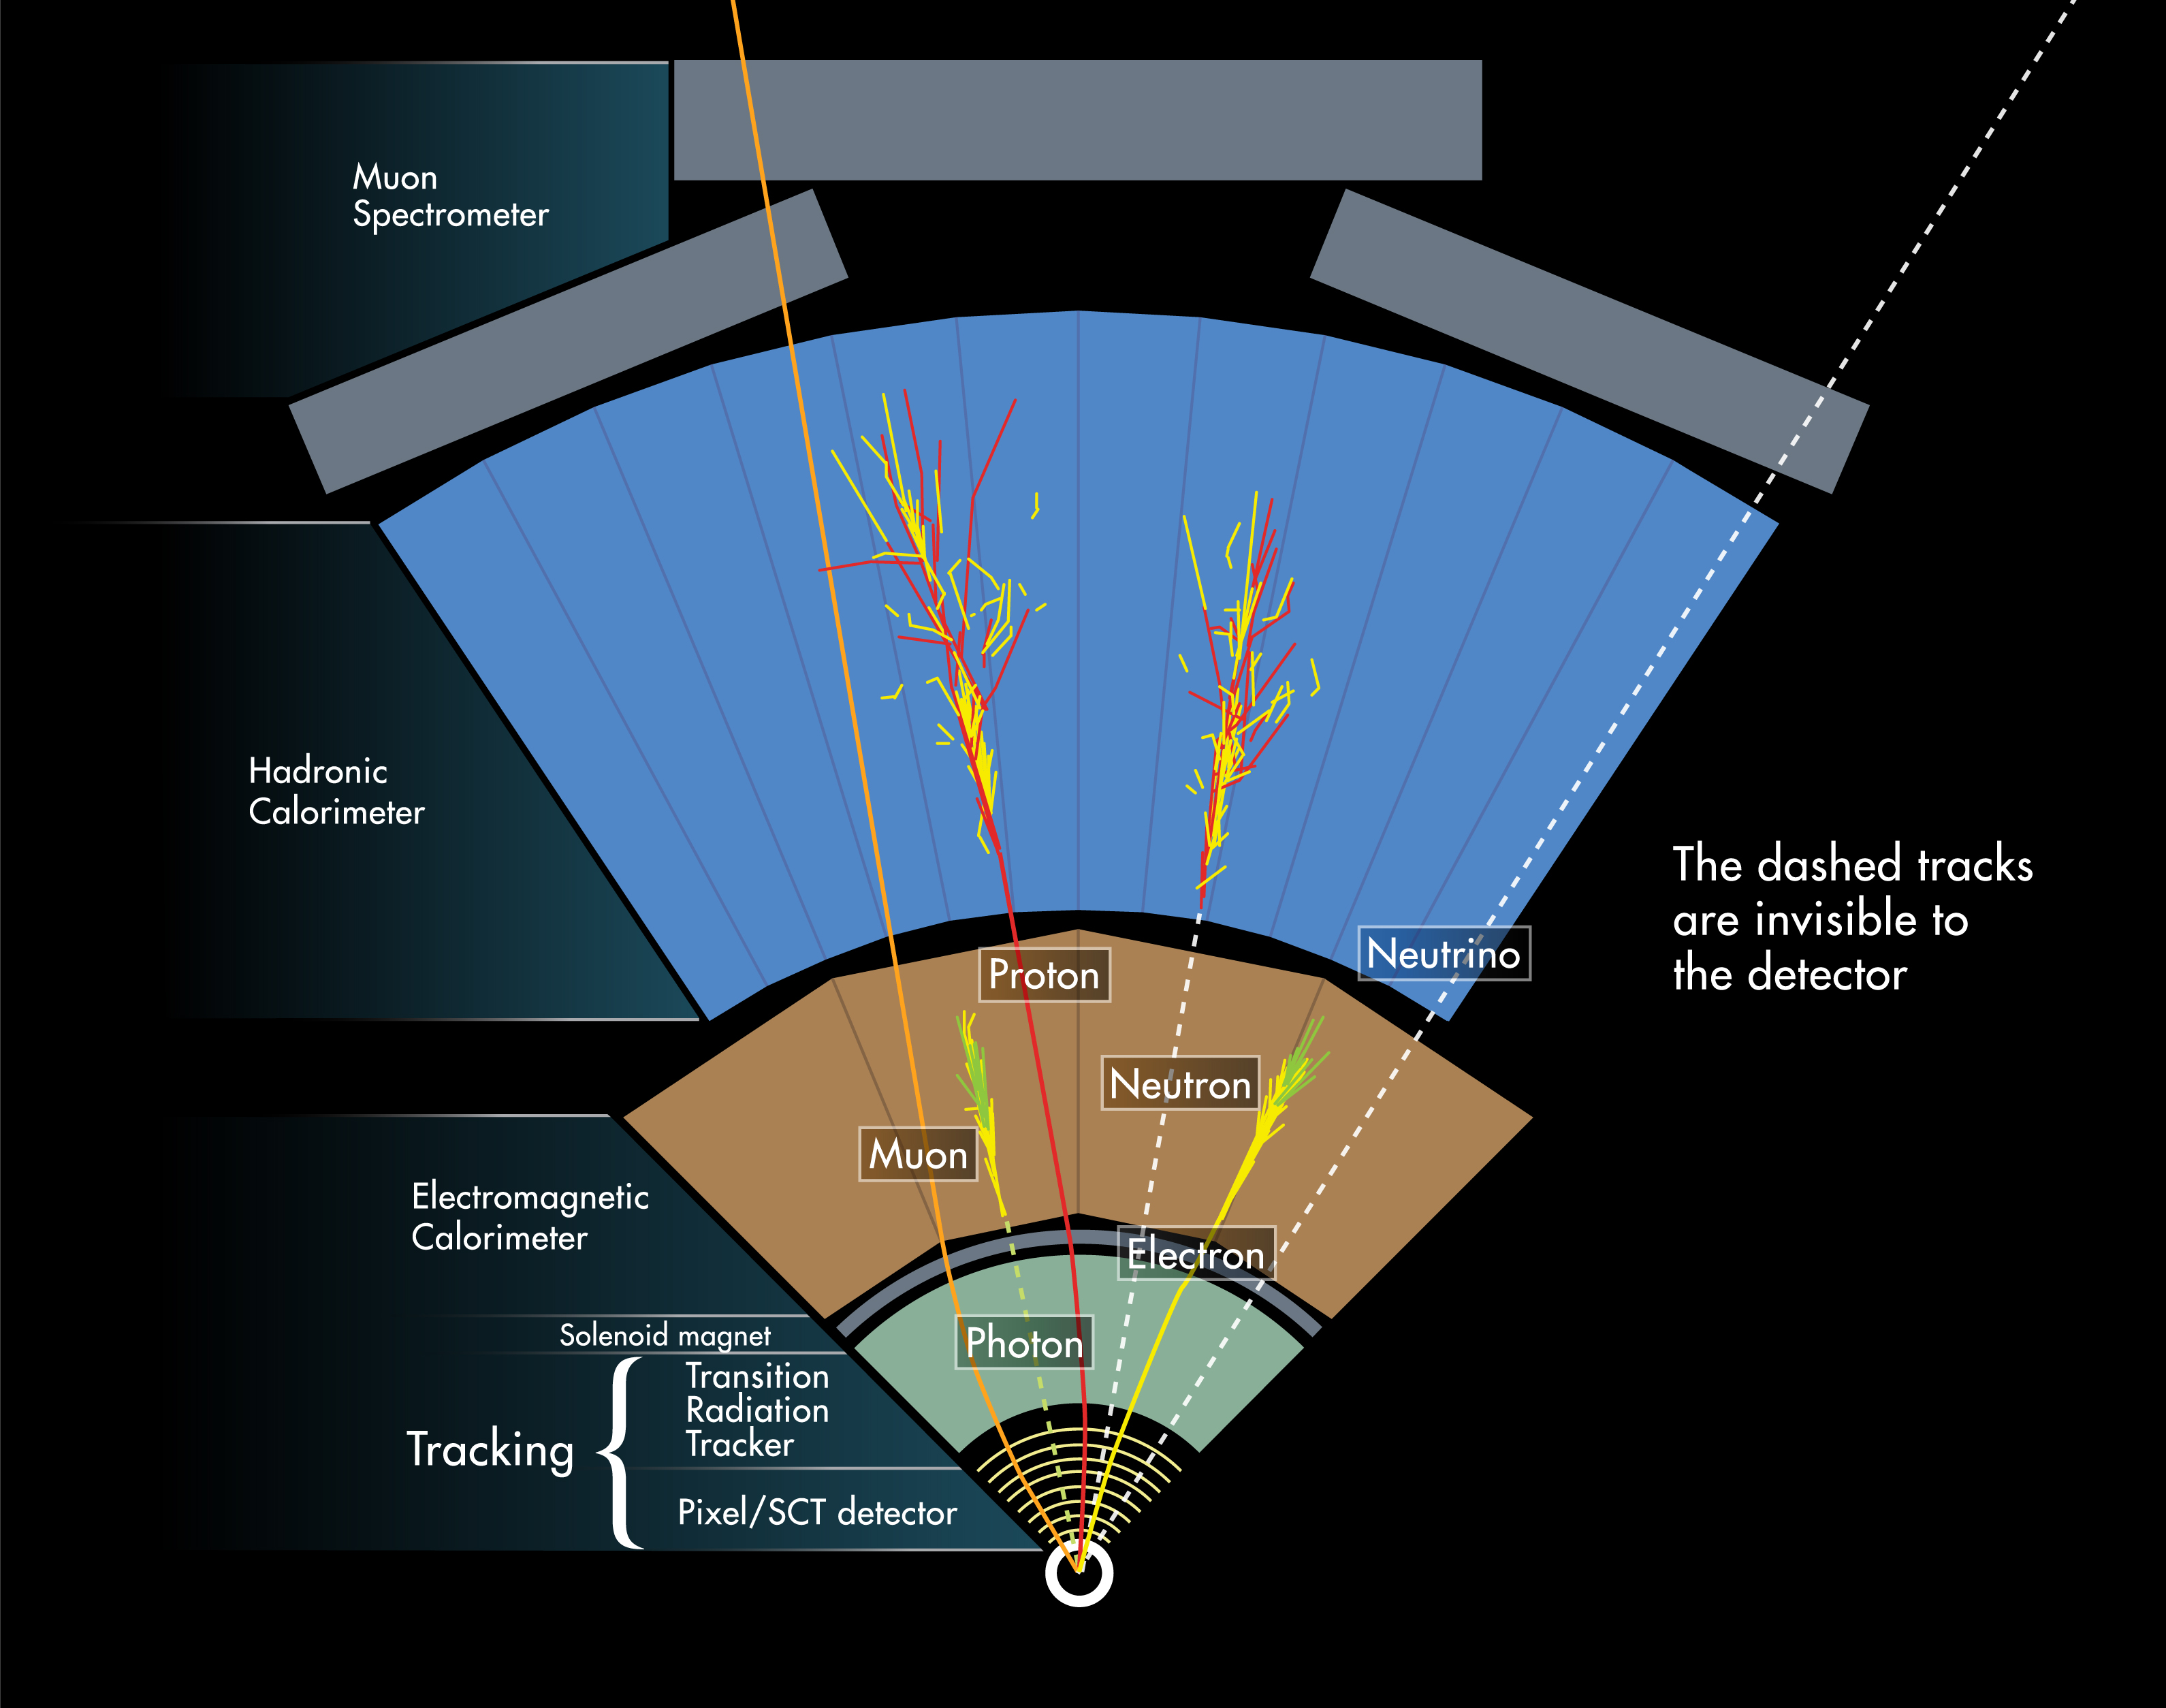
\includegraphics[width=0.95\textwidth]
    {figures/lhc_and_atlas/particle_signatures.jpg}
  \end{center}
\end{frame}

% ==============================================================================
\section{\BMINUSL\ search}

% ------------------------------------------------------------------------------
\begin{frame}
  \frametitle{Analysis strategy}
  \UpdateFlag
  %%
\end{frame}

% ------------------------------------------------------------------------------
\begin{frame}
  \frametitle{Object selection}
  \UpdateFlag
  %%
\end{frame}

% ------------------------------------------------------------------------------
\begin{frame}
  \frametitle{Triggers}
  \UpdateFlag
  %%
\end{frame}

% ------------------------------------------------------------------------------
\begin{frame}
  \frametitle{Selection criteria}
  \UpdateFlag
  %%
\end{frame}

% ==============================================================================
\subsection{Results}

% ------------------------------------------------------------------------------
\begin{frame}
  \frametitle{Results}
  \UpdateFlag
  %%
\end{frame}

% ==============================================================================
\section{Conclusions}

% ------------------------------------------------------------------------------
\begin{frame}
  \frametitle{Conclusions}
  \UpdateFlag
  %%
\end{frame}

% ------------------------------------------------------------------------------
\begin{frame}
  \begin{center}
    {\Huge \color{RoyalBlue} Backup}
  \end{center}
\end{frame}

%%% %%% % ------------------------------------------------------------------------------
%%% %%% \begin{frame}
%%% %%%   \frametitle{Introduction}
%%% %%%   \begin{itemize}
%%% %%%     \item Working with theorists at Penn, we are interested in
%%% %%%       {\color{blue} \textbf{stop pair production}}
%%% %%%       \begin{itemize}
%%% %%%         \item The stop decays to a {\color{red} \textbf{b-quark + lepton}}
%%% %%%         \item Search for final states with
%%% %%%           {\color{red} $ee bb$, $\mu\mu bb$, $e\mu bb$}
%%% %%%         \item Looking for a {\color{blue} resonance in the invariant mass of
%%% %%%             the lepton and b-quark
%%% %%%           }
%%% %%%       \end{itemize}
%%% %%%     \item Support note: {\color{blue} \href{https://cds.cern.ch/record/1748654}{https://cds.cern.ch/record/1748654}}
%%% %%%     \item CONF note: {\color{blue} \href{https://cds.cern.ch/record/2001081}{https://cds.cern.ch/record/2001081}}
%%% %%%   \end{itemize}
%%% %%%   %%
%%% %%%   \begin{center}
%%% %%%     \resizebox{0.5\linewidth}{!}{
%%% %%%       \begin{tikzpicture}
%%% %%%         \node[anchor=south west, inner sep=0] (image) at (0,0) {
%%% %%%           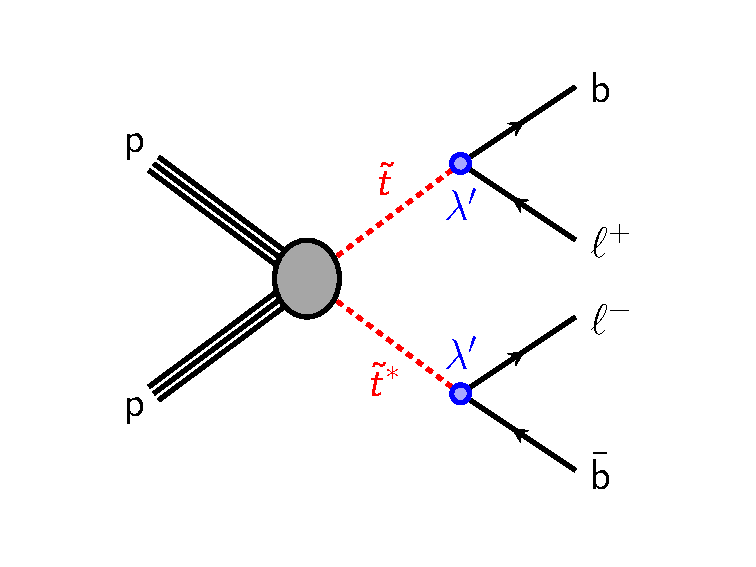
\includegraphics{figures/b_minus_l_stop_stop.pdf}
%%% %%%         };
%%% %%%       \end{tikzpicture}
%%% %%%     }
%%% %%%   \end{center}
%%% %%% 
%%% %%%   \tikzoverlay[text width=3.cm] at (+9.6cm, +1.3cm) {
%%% %%%     \tikz node[text=white] at (0., 0.) {
%%% %%%       \node[rectangle, rounded corners=1ex, text=white, fill=RoyalBlue!30!white] at (0., 0.) {
%%% %%%         \scriptsize
%%% %%%         \begin{center}
%%% %%%           \begin{tabular}{c}
%%% %%%             Theorists at Penn \\
%%% %%%             \midrule
%%% %%%             Professor Burt Ovrut \\
%%% %%%             Dr. Sogee Spinner \\
%%% %%%             Mr. Austin Purves
%%% %%%           \end{tabular}
%%% %%%         \end{center}
%%% %%%       };
%%% %%%     };
%%% %%%   };
%%% %%% \end{frame}
%%% %%% 
%%% %%% 
%%% %%% %% % ------------------------------------------------------------------------------
%%% %%% \begin{frame}
%%% %%%   \frametitle{Model}
%%% %%%   %%
%%% %%%   \begin{center}
%%% %%%       \begin{tikzpicture}
%%% %%%         \node[anchor=south west, inner sep=0] (image) at (0,0) {
%%% %%%           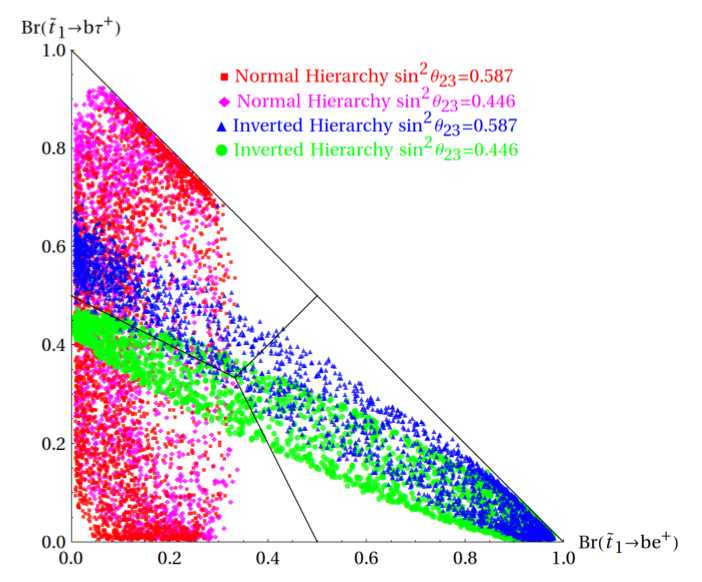
\includegraphics[width=0.5\linewidth]{figures/stop_model_scan.png}
%%% %%%         };
%%% %%%         \begin{scope}[x={(image.south east)}, y={(image.north west)}]
%%% %%%           \node[rectangle, rounded corners=1ex, fill=RoyalBlue!30!white] at (0.65, 0.95) {
%%% %%%             \scriptsize \href{http://arxiv.org/abs/1401.7989}{http://arxiv.org/abs/1401.7989}
%%% %%%           };
%%% %%%           % \node[rectangle, rounded corners=1ex, minimum width=2cm, minimum height=0.5cm, fill=RoyalBlue!80!white, text=white] at (0.85, 0.2) {
%%% %%%           \node[rectangle, rounded corners=1ex, fill=RoyalBlue!80!white, text=white] at (0.95, 0.2) {
%%% %%%             Mostly $ee$
%%% %%%           };
%%% %%%           \node[rectangle, rounded corners=1ex, fill=RoyalBlue!80!white, text=white] at (-0.15, 0.2) {
%%% %%%             Mostly $\mu\mu$
%%% %%%           };
%%% %%%           \node[rectangle, rounded corners=1ex, fill=ForestGreen!80!white, text=white] at (0.85, 0.5) {
%%% %%%             \footnotesize
%%% %%%             \begin{tabular}{c}
%%% %%%               Branching ratios of \\
%%% %%%               $\tilde{t}\rightarrow b\ell$ related to \\
%%% %%%               neutrino hierarchy
%%% %%%             \end{tabular}
%%% %%%           };
%%% %%% 
%%% %%%           % \MyGrid
%%% %%% 
%%% %%%         \end{scope}
%%% %%%       \end{tikzpicture}
%%% %%%   \end{center}
%%% %%%   %%
%%% %%%   \begin{itemize}
%%% %%%     \item Gauged \BMINUSL\ extension of MSSM
%%% %%%       \begin{itemize}
%%% %%%         \item Minimal additional particle content (MSSM+right-handed neutrinos)
%%% %%%         \item Automatically leads to R-parity violation
%%% %%%       \end{itemize}
%%% %%%     \item If the stop is the LSP, the allowed decays are:
%%% %%%       \begin{itemize}
%%% %%%         \item {\color{blue} $\tilde{t} \rightarrow b\ell$ (favored for most of
%%% %%%           parameter space)}
%%% %%%         \item $\tilde{t} \rightarrow t\nu$ (negligible unless purely right-handed stop)
%%% %%%       \end{itemize}
%%% %%%     \item Differs from leptoquark searches because we require a b-tagged jet and a light lepton
%%% %%%   \end{itemize}
%%% %%%   %%
%%% %%% \end{frame}
%%% %%% 
%%% %%% 
%%% %%% % ------------------------------------------------------------------------------
%%% %%% \begin{frame}
%%% %%%   \frametitle{Analysis strategy}
%%% %%%   %%
%%% %%%   \begin{center}
%%% %%%     \begin{tikzpicture}
%%% %%%       \node[anchor=south west, inner sep=0] (image) at (0,0) {
%%% %%%         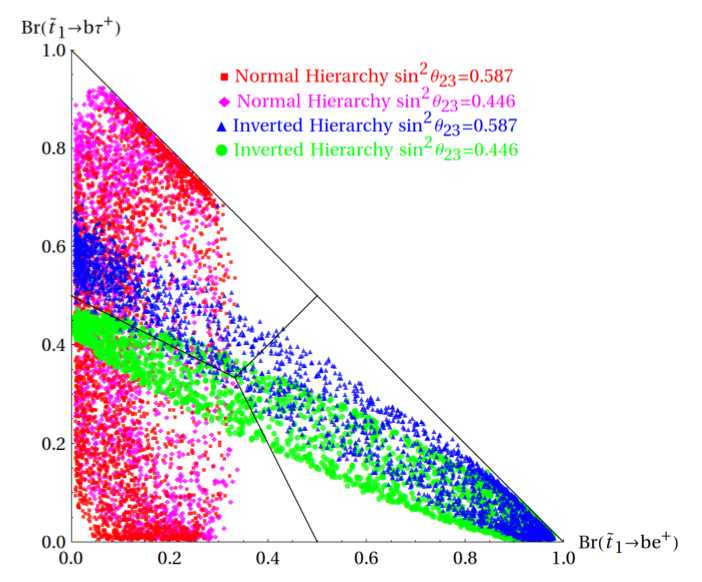
\includegraphics[width=0.5\linewidth]{figures/stop_model_scan.png}
%%% %%%       };
%%% %%%       \begin{scope}[x={(image.south east)}, y={(image.north west)}]
%%% %%%         \fill[fill=MidnightBlue!80!white] (0.45,0.075) circle (0.5ex);
%%% %%%         % \node[rectangle, rounded corners=1ex, minimum width=2cm, minimum height=0.5cm, fill=RoyalBlue!80!white, text=white] at (0.85, 0.2) {
%%% %%%         \node[rectangle, rounded corners=1ex, fill=RoyalBlue!80!white, text=white] at (0.95, 0.2) {
%%% %%%           Mostly $ee$
%%% %%%         };
%%% %%%         \node[rectangle, rounded corners=1ex, fill=RoyalBlue!80!white, text=white] at (-0.15, 0.2) {
%%% %%%           Mostly $\mu\mu$
%%% %%%         };
%%% %%%         \node[rectangle, rounded corners=1ex, fill=ForestGreen!80!white, text=white] at (0.93, 0.5) {
%%% %%%           \footnotesize
%%% %%%           \begin{tabular}{c}
%%% %%%             Increasing the \\
%%% %%%             branching ratio to \\
%%% %%%             $b\tau$ leads to fewer \\
%%% %%%             observable events
%%% %%%           \end{tabular}
%%% %%%         };
%%% %%%         \draw[->, ForestGreen!80!white, ultra thick] (0.65, 0.3) to (0.40, 0.60);
%%% %%%         % \MyGrid
%%% %%%       \end{scope}
%%% %%%     \end{tikzpicture}
%%% %%%   \end{center}
%%% %%%   \begin{itemize}
%%% %%%     \item Simplified signal Monte Carlo samples using
%%% %%%       {\color{blue} \textbf{Madgraph + Pythia}}
%%% %%%       \begin{itemize}
%%% %%%         \item $Br(\Stop \rightarrow be) = Br(\Stop \rightarrow b\mu) = 0.5$
%%% %%%         \item Cross sections are NLO (same as traditional stop production)
%%% %%%       \end{itemize}
%%% %%%     \item Looking for an excess at high \Mbl
%%% %%%     \item In absence of observable signal, {\color{red} place lower limit} on
%%% %%%       the allowed stop mass
%%% %%%     \item Can sample the full plane of branching ratios by scaling the flavor
%%% %%%       channels up and down
%%% %%%   \end{itemize}
%%% %%%   %%
%%% %%% \end{frame}
%%% %%% 
%%% %%% 
%%% %%% % ------------------------------------------------------------------------------
%%% %%% \begin{frame}
%%% %%%   \frametitle{Search strategy}
%%% %%%   %%
%%% %%%   \begin{columns}
%%% %%%     \column{0.6\textwidth}
%%% %%%     \begin{itemize}
%%% %%%       \item Selecting final states with
%%% %%%         \begin{itemize}
%%% %%%           \item {\color{blue}Two leptons} ($e/\mu$)
%%% %%%           \item {\color{red}Two b-tagged jets}
%%% %%%         \end{itemize}
%%% %%%       \item Define {\color{blue}\textbf{two signal regions}} with high signal
%%% %%%         efficiency and low expected background contamination
%%% %%%       \item {\color{red} Dedicated Control regions} to constrain \TTBAR\ and
%%% %%%         \ZGAMMA\ backgrounds
%%% %%%       \item Other backgrounds taken from MC
%%% %%%       \item For each choice of branching ratio, select region with the
%%% %%%         {\color{blue} \textbf{best expected sensitivity}}
%%% %%%     \end{itemize}
%%% %%%     %%
%%% %%%     \column{0.4\textwidth}
%%% %%%     \begin{block}{Signal}
%%% %%%       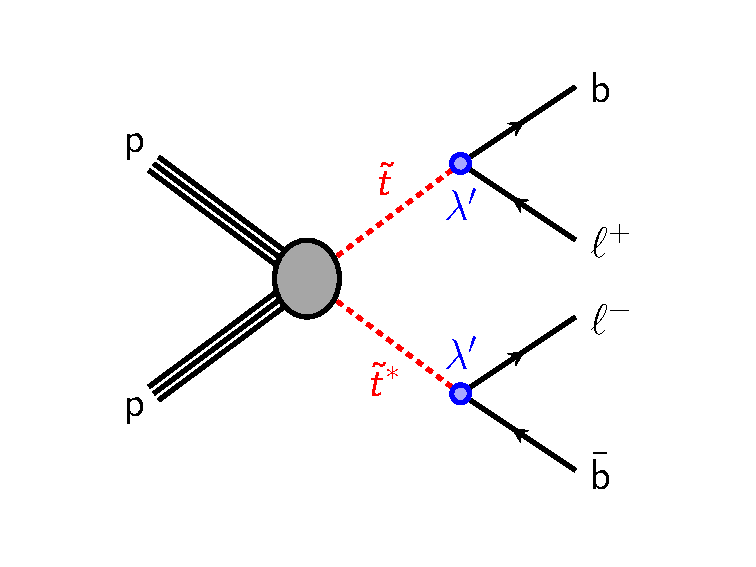
\includegraphics[width=\textwidth]{figures/b_minus_l_stop_stop.pdf}
%%% %%%     \end{block}
%%% %%%     \begin{block}{Background}
%%% %%%       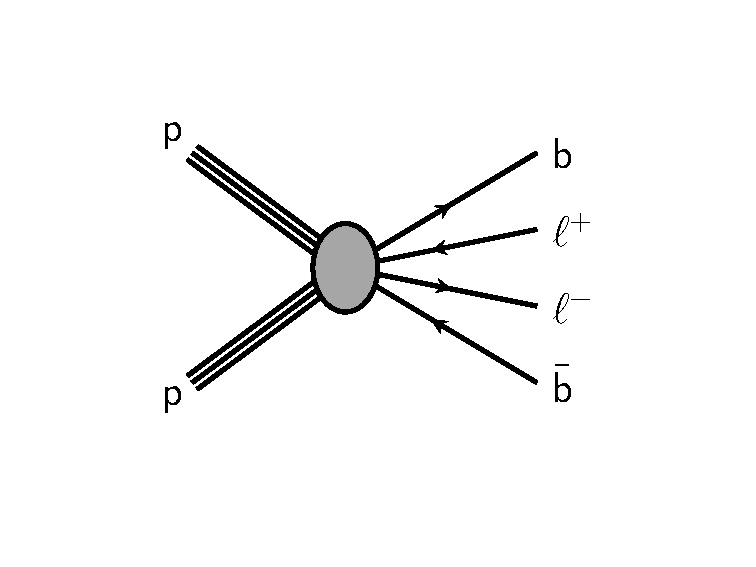
\includegraphics[width=\textwidth]{figures/generic_bbll.pdf}
%%% %%%     \end{block}
%%% %%%   \end{columns}
%%% %%% \end{frame}
%%% %%% 
%%% %%% 
%%% %%% % ------------------------------------------------------------------------------
%%% %%% \begin{frame}
%%% %%%   \frametitle{Selection}
%%% %%%   %%
%%% %%%   \begin{columns}
%%% %%%     \column{0.4\textwidth}
%%% %%%     \begin{block}{Baseline objects}
%%% %%%       \vspace{1ex}
%%% %%%       \resizebox{\textwidth}{!}{
%%% %%%         \begin{tabular}{c|ccc}
%%% %%%           \toprule
%%% %%%           Variable                                     & Electrons & Muons   & Jets          \\
%%% %%%           \toprule
%%% %%%           ID                                           & Medium++  & Loose   & AntiKt4LCTopo \\
%%% %%%           $p_{\mathrm{T}}$ [GeV]                       & $> 40$    & $> 40$  & $> 40$        \\
%%% %%%           $|\eta|$                                     & $< 2.47$  & $< 2.4$ & $< 4.5$       \\
%%% %%%           $\left| \frac{d_{0}}{\sigma(d_{0})} \right|$ & $< 3$     & $< 3$   & -             \\
%%% %%%           $z_{0}\text{sin}(\theta)$ [mm]               & $< 0.4$   & $< 1$   & -             \\
%%% %%%           \bottomrule
%%% %%%         \end{tabular}
%%% %%%       }
%%% %%%     \end{block}
%%% %%%     \begin{block}{Overlap removal}
%%% %%%       \vspace{1ex}
%%% %%%       \resizebox{\textwidth}{!}{
%%% %%%         \begin{tabular}{lcl}
%%% %%%           \toprule
%%% %%%           Objects & Cut & Remove \\
%%% %%%           \midrule
%%% %%%           $ee$      & $\Delta R \le$ 0.05                        & Lower $E_{T}$ electron             \\
%%% %%%           jet $e$   & $\Delta R \le$ 0.20                        & Jet                                \\
%%% %%%           jet $e$   & $\Delta R \le$ 0.40                        & Electron                           \\
%%% %%%           jet $\mu$ & $\Delta R \le$ 0.40                        & Muon                               \\
%%% %%%           $e\mu$    & $\Delta R \le$ 0.01                        & Electron and muon                  \\
%%% %%%           $\mu\mu$  & $\Delta R \le$ 0.05                        & Both muons                         \\
%%% %%%           \midrule
%%% %%%           SF OS     & \multirow{2}{*}{$m_{\ell\ell} \le 12$ GeV} & \multirow{2}{*}{Electron and muon} \\
%%% %%%           leptons   &                                            & \\
%%% %%%           \bottomrule
%%% %%%         \end{tabular}
%%% %%%       }
%%% %%%     \end{block}
%%% %%%     \begin{block}{Signal objects}
%%% %%%       \vspace{1ex}
%%% %%%       \resizebox{\textwidth}{!}{
%%% %%%         \begin{tabular}{c|ccc}
%%% %%%           \toprule
%%% %%%           Variable & Electrons & Muons   & Jets\\
%%% %%%           \toprule
%%% %%%           $|\eta|$ & $\le 2.47$  & $\le 2.4$ & $\le 2.4$ \\
%%% %%%           $p_\mathrm{T}^{\mathrm{cone}30}/\min(p_\mathrm{T}, 60)$ &
%%% %%%             $\le 0.1$ &
%%% %%%             $\le 0.1$ & - \\
%%% %%%           B-Tag working point & - & - & 80 \% \\
%%% %%%           \bottomrule
%%% %%%         \end{tabular}
%%% %%%       }
%%% %%%     \end{block}
%%% %%%     %%
%%% %%%     \column{0.6\textwidth}
%%% %%%     \begin{itemize}
%%% %%%       \item Much of selection based on EWK SS analysis
%%% %%%       \item Apply basic event cleaning
%%% %%%         \begin{itemize}
%%% %%%           \item Jet cleaning, cosmic muon veto, etc
%%% %%%         \end{itemize}
%%% %%%       \item Require at least two leptons with opposite charge and two
%%% %%%         b-tagged jets
%%% %%%         \begin{itemize}
%%% %%%           \item Select two leading lepton and two leading b-tagged jets if
%%% %%%             there are more than two of each
%%% %%%         \end{itemize}
%%% %%%       \item Two possible pairings for $bb\ell\ell$ system
%%% %%%         \begin{center}
%%% %%%           \resizebox{0.80\textwidth}{!}{%
%%% %%%             \begin{tikzpicture}
%%% %%%               \node[rectangle, text=black] (sel1) at (-5.0,+0.5) {Selection 1:};
%%% %%%               \node[rectangle, text=black] (sel2) at (-5.0,-0.5) {Selection 2:};
%%% %%% 
%%% %%%               \node[rectangle, rounded corners=1ex, fill=pairing_b_1, text=black] (b1) at (-3.25,+0.5) {$b_0$};
%%% %%%               \node[rectangle, rounded corners=1ex, fill=pairing_l_1, text=black] (l1) at (-2.50,+0.5) {$\ell_0$};
%%% %%%               \node[rectangle, rounded corners=1ex, fill=pairing_b_2, text=black] (b2) at (+1.25,+0.5) {$b_1$};
%%% %%%               \node[rectangle, rounded corners=1ex, fill=pairing_l_2, text=black] (l2) at (+2.00,+0.5) {$\ell_1$};
%%% %%%               \node[rectangle, text=black] (m11) at (-1.0,+0.5) {$\Rightarrow m_{b1\ell1} = m_{b\ell}^{0}$};
%%% %%%               \node[rectangle, text=black] (m22) at (+3.5,+0.5) {$\Rightarrow m_{b2\ell2} = m_{b\ell}^{1}$};
%%% %%% 
%%% %%%               \node[rectangle, rounded corners=1ex, fill=pairing_b_1, text=black] (b1) at (-3.25,-0.5) {$b_0$};
%%% %%%               \node[rectangle, rounded corners=1ex, fill=pairing_l_2, text=black] (l2) at (-2.50,-0.5) {$\ell_1$};
%%% %%%               \node[rectangle, rounded corners=1ex, fill=pairing_b_2, text=black] (b2) at (+1.25,-0.5) {$b_1$};
%%% %%%               \node[rectangle, rounded corners=1ex, fill=pairing_l_1, text=black] (l1) at (+2.00,-0.5) {$\ell_0$};
%%% %%%               \node[rectangle, text=black] (m12) at (-1.0,-0.5) {$\Rightarrow m_{b1\ell2} = m_{b\ell}^{0} $};
%%% %%%               \node[rectangle, text=black] (m21) at (+3.5,-0.5) {$\Rightarrow m_{b2\ell1} = m_{b\ell}^{1} $};
%%% %%%             \end{tikzpicture}
%%% %%%           }
%%% %%%         \end{center}
%%% %%%       \item Choose pairing with smallest difference in mass between two pairs
%%% %%%     \end{itemize}
%%% %%%     %%
%%% %%%   \end{columns}
%%% %%% \end{frame}
%%% %%% 
%%% %%% 
%%% %%% % ------------------------------------------------------------------------------
%%% %%% \begin{frame}
%%% %%%   \frametitle{Trigger}
%%% %%%   %%
%%% %%%   \begin{center}
%%% %%%     \begin{tikzpicture}
%%% %%%       \node[anchor=south west, inner sep=0] (image) at (0,0) {
%%% %%%         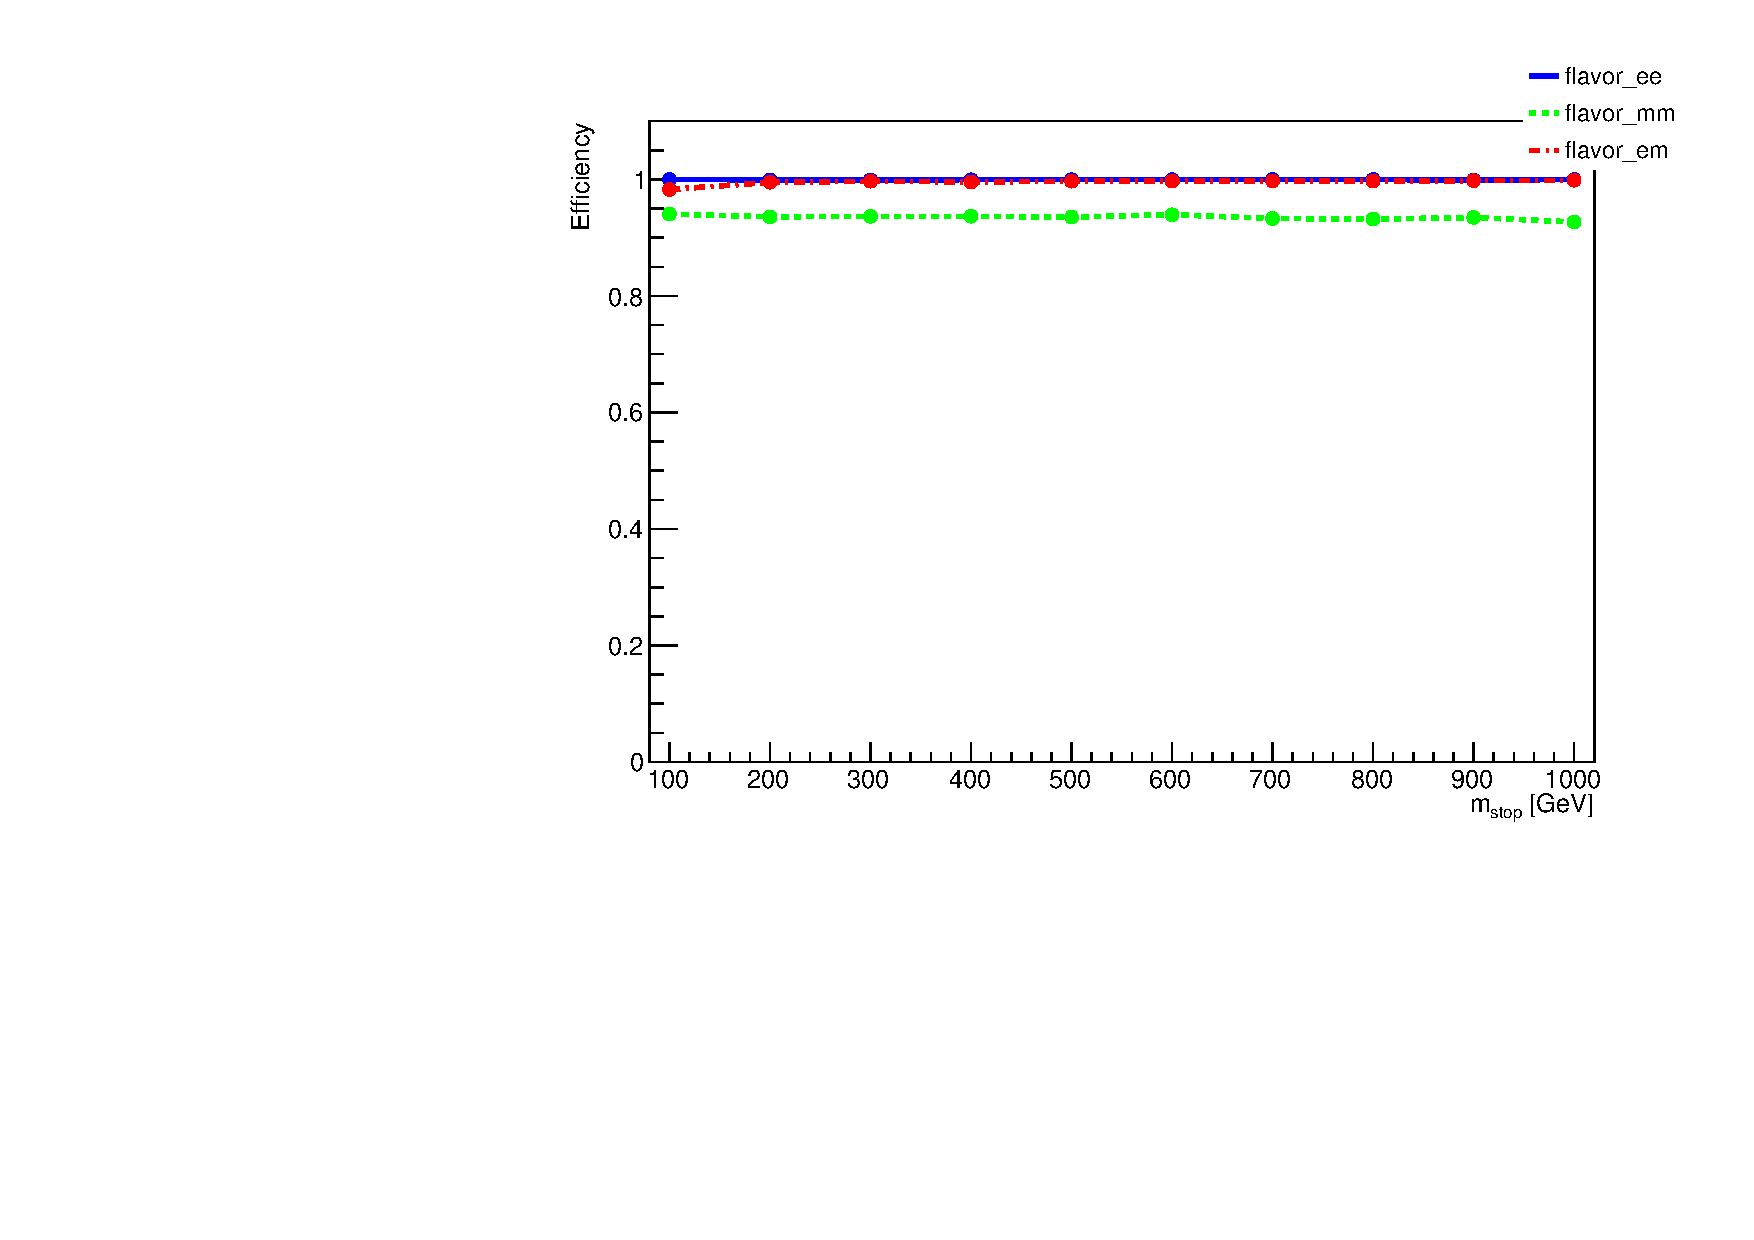
\includegraphics[width=0.6\linewidth]{figures/EF_e24vhi_medium1_OR_EF_e60_medium1_OR_EF_mu36_tight.pdf}
%%% %%%       };
%%% %%%       \begin{scope}[x={(image.south east)}, y={(image.north west)}]
%%% %%%         % \node[rectangle, rounded corners=1ex, minimum width=2cm, minimum height=0.5cm, fill=RoyalBlue!80!white, text=white] at (0.85, 0.2) {
%%% %%%         \node[rectangle, rounded corners=1ex, fill=RoyalBlue!80!white, text=white] at (0.95, 0.5) {
%%% %%%           \footnotesize
%%% %%%           \begin{tabular}{c}
%%% %%%             e24vhi\\
%%% %%%             e60 \\
%%% %%%             mu24i \\
%%% %%%             mu36
%%% %%%           \end{tabular}
%%% %%%         };
%%% %%%         % \MyGrid
%%% %%%       \end{scope}
%%% %%%     \end{tikzpicture}
%%% %%%   \end{center}
%%% %%%   %%
%%% %%%   \begin{itemize}
%%% %%%     \item We use the {\color{blue}\textbf{or}} of several
%%% %%%       {\color{blue}\textbf{single lepton triggers}}
%%% %%%     \item The trigger selection depends on the flavor channel
%%% %%%       \begin{itemize}
%%% %%%         \item $ee$ events: {\color{blue}\textbf{e24vhi}} or
%%% %%%           {\color{blue}\textbf{e60}}
%%% %%%         \item $\mu\mu$ events: {\color{blue}\textbf{mu24i}} or
%%% %%%           {\color{blue}\textbf{mu36}}
%%% %%%         \item $e\mu$ events: {\color{blue}\textbf{e24vhi}} or
%%% %%%           {\color{blue}\textbf{e60}} or
%%% %%%           {\color{blue}\textbf{mu24i}} or
%%% %%%           {\color{blue}\textbf{mu36}}
%%% %%%       \end{itemize}
%%% %%%     \item Require one of the selected leptons to be matched to a trigger object
%%% %%%       ({\color{blue}$\Delta R \le 0.15$})
%%% %%%   \end{itemize}
%%% %%% \end{frame}
%%% %%% 
%%% %%% 
%%% %%% % ------------------------------------------------------------------------------
%%% %%% \frame
%%% %%% {
%%% %%%   \frametitle{Region definitions}
%%% %%%   \begin{center}
%%% %%%     \resizebox{\textwidth}{!}{
%%% %%%       \begin{tabular}{l|ccccc}
%%% %%%         \toprule
%%% %%%         Region &
%%% %%%         $\Mbl^0$ [GeV] &
%%% %%%         \Ht [GeV] &
%%% %%%         \MetSig\ [$\mathrm{GeV}^{1/2}$] &
%%% %%%         \MblAsym &
%%% %%%         Z region \\
%%% %%%         \midrule
%%% %%%         SR 400   & $\ge 400$  & $\ge 1100$ & --      & $\le 0.2$ & Veto   \\
%%% %%%         SR 600   & $\ge 600$  & $\ge 1100$ & --      & $\le 0.2$ & Veto   \\
%%% %%%         \midrule
%%% %%%         Top CR   & $\ge 200$  & $\le 500$  & $\ge 4$ & $\le 0.2$ & Veto   \\
%%% %%%         Z CR     & $\ge 200$  & $\le 500$  & $\le 4$ & $\le 0.2$ & Select \\
%%% %%%         \midrule
%%% %%%         Top VR 1 & $\ge 200$  & $\le 500$  & $\le 4$ & $\le 0.2$ & Veto   \\
%%% %%%         Top VR 2 & $\ge 200$  & $\le 500$  & -       & $\ge 0.2$ & Veto   \\
%%% %%%         Top VR 3 & $\ge 200$  & $\ge 500$  & $\ge 4$ & $\ge 0.2$ & Veto   \\
%%% %%%         Z VR     & $\ge 200$  & $\ge 500$  & --      & $\le 0.2$ & Select \\
%%% %%%         \bottomrule
%%% %%%       \end{tabular}
%%% %%%     }
%%% %%%   \end{center}
%%% %%% 
%%% %%%   \begin{columns}
%%% %%%     \column{0.5\textwidth}
%%% %%%     \begin{itemize}
%%% %%%       \item The Z region is defined to be events with two same-flavor leptons
%%% %%%         with invariant mass $|m_{\ell\ell} - m_Z| \le 10$ GeV
%%% %%%       \item Signal regions optimized for stops with fairly high masses
%%% %%%     \end{itemize}
%%% %%%     %%
%%% %%%     \column{0.5\textwidth}
%%% %%%     \[
%%% %%%       \Ht = \sum_{i=1}^{2} p_T^{\ell_i} + \sum_{j=1}^{2} p_T^{\mathrm{b~jet}_j}
%%% %%%     \]
%%% %%%     \[
%%% %%%       \MblAsym = 
%%% %%%       \frac{\left(\Mbl^0-\Mbl^1\right)}{\left(\Mbl^0+\Mbl^1\right)}
%%% %%%     \]
%%% %%%     \[
%%% %%%       \MetSig = \frac{\Met}{\sqrt{\Ht}}
%%% %%%     \]
%%% %%%     %%
%%% %%%   \end{columns}
%%% %%% }
%%% %%% 
%%% %%% 
%%% %%% % ------------------------------------------------------------------------------
%%% %%% \frame
%%% %%% {
%%% %%%   \frametitle{Region definitions}
%%% %%%   \begin{figure}
%%% %%%     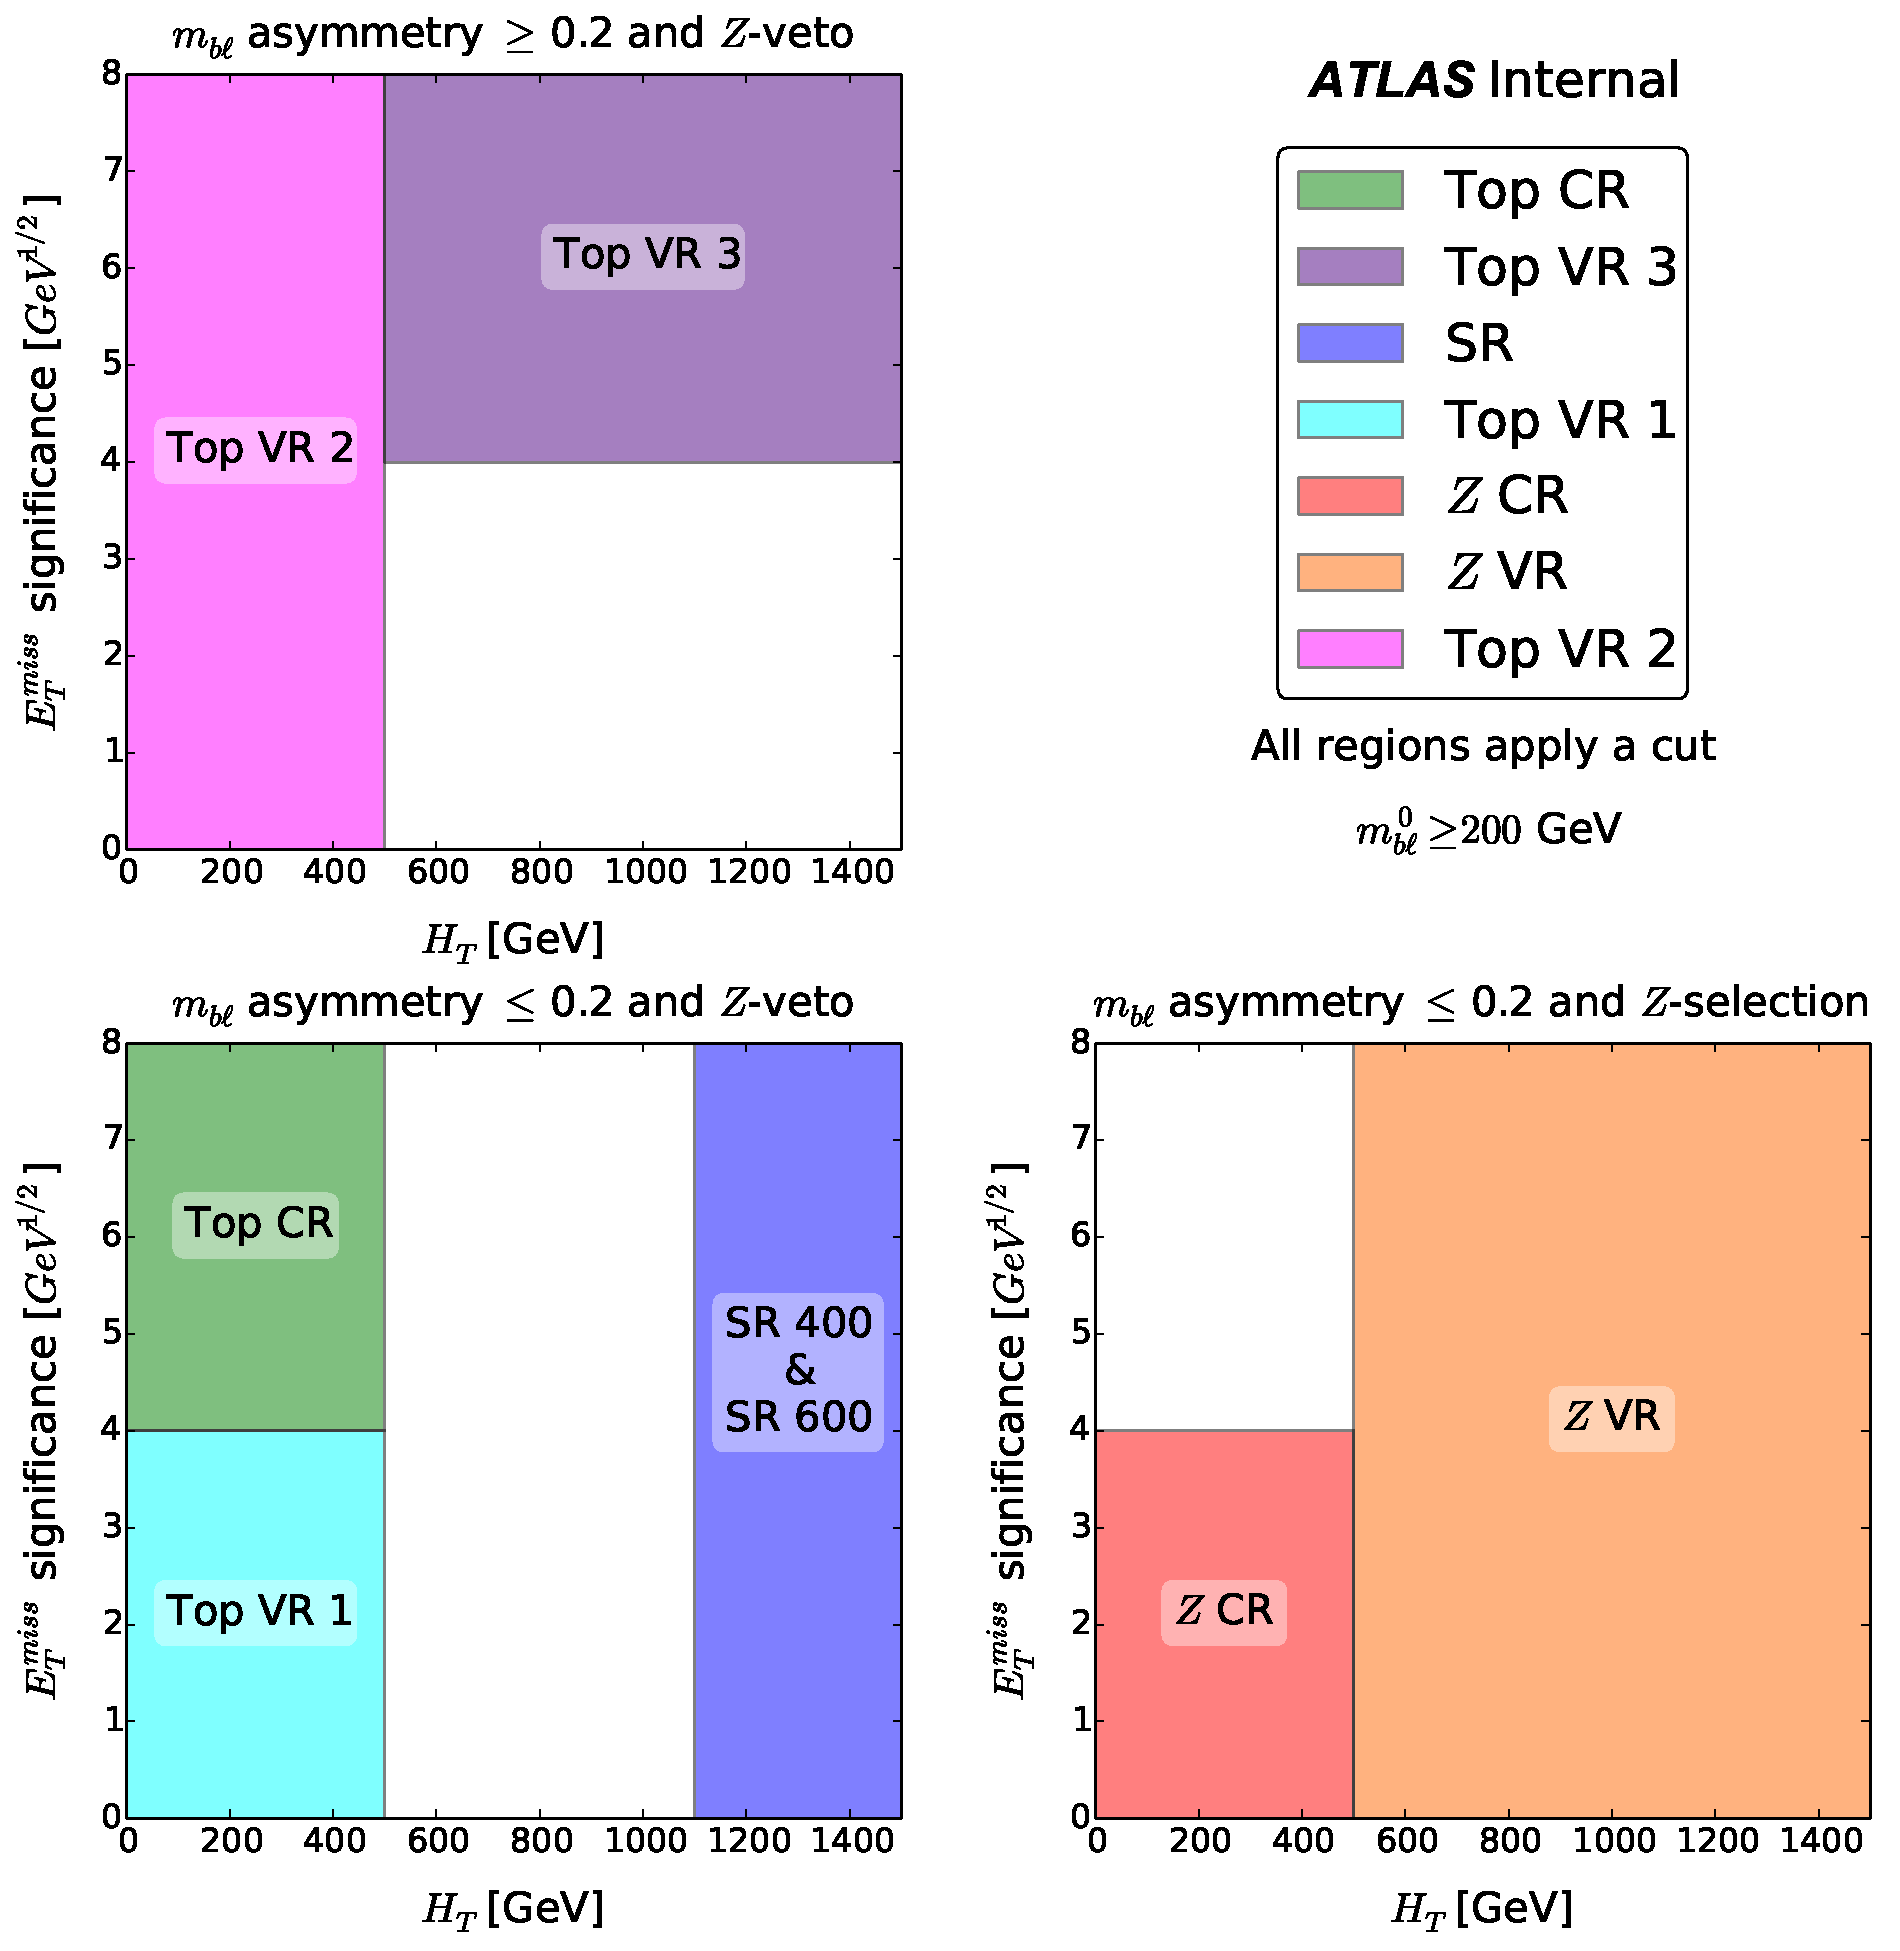
\includegraphics[height=0.80\textheight]{figures/regions__met_sig__ht_plane.pdf}
%%% %%%   \end{figure}
%%% %%% }
%%% %%% 
%%% %%% 
%%% %%% % ------------------------------------------------------------------------------
%%% %%% \begin{frame}
%%% %%%   \frametitle{Signal region}
%%% %%%   \begin{columns}
%%% %%%     \column{0.5\textwidth}
%%% %%%     \begin{table}
%%% %%%       \resizebox{\textwidth}{!}{
%%% %%%         \begin{tabular}{c|cc}
%%% %%%           \toprule
%%% %%%                                                & SR 400                & SR 600 \\
%%% %%%           \midrule
%%% %%%           $t\bar{t}$                           & $0.3$                 & $8.9 \cdot 10^{-2}$ \\
%%% %%%           $Z/\gamma^{*}$                       & $0.5$                 & $0.2$ \\
%%% %%%           Single top                           & $0.4$                 & $0.2$ \\
%%% %%%           Other                                & $6.9 \cdot 10^{-2}$   & $4.2 \cdot 10^{-2}$ \\
%%% %%%           \midrule
%%% %%%           Total                                & $1.3$                 & $0.5$ \\
%%% %%%           background                           & ($\pm$ $0.2$)         & ($\pm$ $0.1$) \\
%%% %%%           \midrule
%%% %%%           \multirow{2}{*}{\BMINUSL\ stop (500 GeV)}  & $110.3$               & $7.7$ \\
%%% %%%                                                & ($82.4$)              & ($14.4$)
%%% %%%           \vspace{1ex} \\
%%% %%%           \multirow{2}{*}{\BMINUSL\ stop (600 GeV)}  & $70.8$                & $34.6$ \\
%%% %%%                                                & ($52.9$)              & ($64.6$)
%%% %%%           \vspace{1ex} \\
%%% %%%           \multirow{2}{*}{\BMINUSL\ stop (700 GeV)}  & $33.8$                & $30.5$ \\
%%% %%%                                                & ($25.3$)              & ($56.8$)
%%% %%%           \vspace{1ex} \\
%%% %%%           \multirow{2}{*}{\BMINUSL\ stop (800 GeV)}  & $13.7$                & $12.9$ \\
%%% %%%                                                & ($10.3$)              & ($24.0$)
%%% %%%           \vspace{1ex} \\
%%% %%%           \multirow{2}{*}{\BMINUSL\ stop (900 GeV)}  & $5.5$                 & $5.2$ \\
%%% %%%                                                & ($4.1$)               & ($9.6$)
%%% %%%           \vspace{1ex} \\
%%% %%%           \multirow{2}{*}{\BMINUSL\ stop (1000 GeV)} & $2.1$                 & $2.0$ \\
%%% %%%                                                & ($1.6$)               & ($3.7$)
%%% %%%           \vspace{1ex} \\
%%% %%%           \bottomrule
%%% %%%         \end{tabular}
%%% %%%       }
%%% %%%     \end{table}
%%% %%%     \column{0.5\textwidth}
%%% %%%     \begin{itemize}
%%% %%%       \item Expected signal and background yields in the signal regions
%%% %%%       \item Assumed branching ratio of
%%% %%%         $Br(\Stop \rightarrow be) = Br(\Stop \rightarrow b\mu) = 0.5$
%%% %%%       \item Number in parentheses for each signal model is the
%%% %%%         {\color{red}\textbf{expected ratio of signal to background}}
%%% %%%       \item Signal regions provide {\color{blue}\textbf{good separation}}
%%% %%%         of signal and background
%%% %%%     \end{itemize}
%%% %%%   \end{columns}
%%% %%% \end{frame}
%%% %%% 
%%% %%% 
%%% %%% % ------------------------------------------------------------------------------
%%% %%% \begin{frame}[t]
%%% %%%   \frametitle{Signal regions}
%%% %%%   \begin{columns}[t]
%%% %%%     \column{0.43\textwidth}
%%% %%%     \begin{block}{\Ht}
%%% %%%       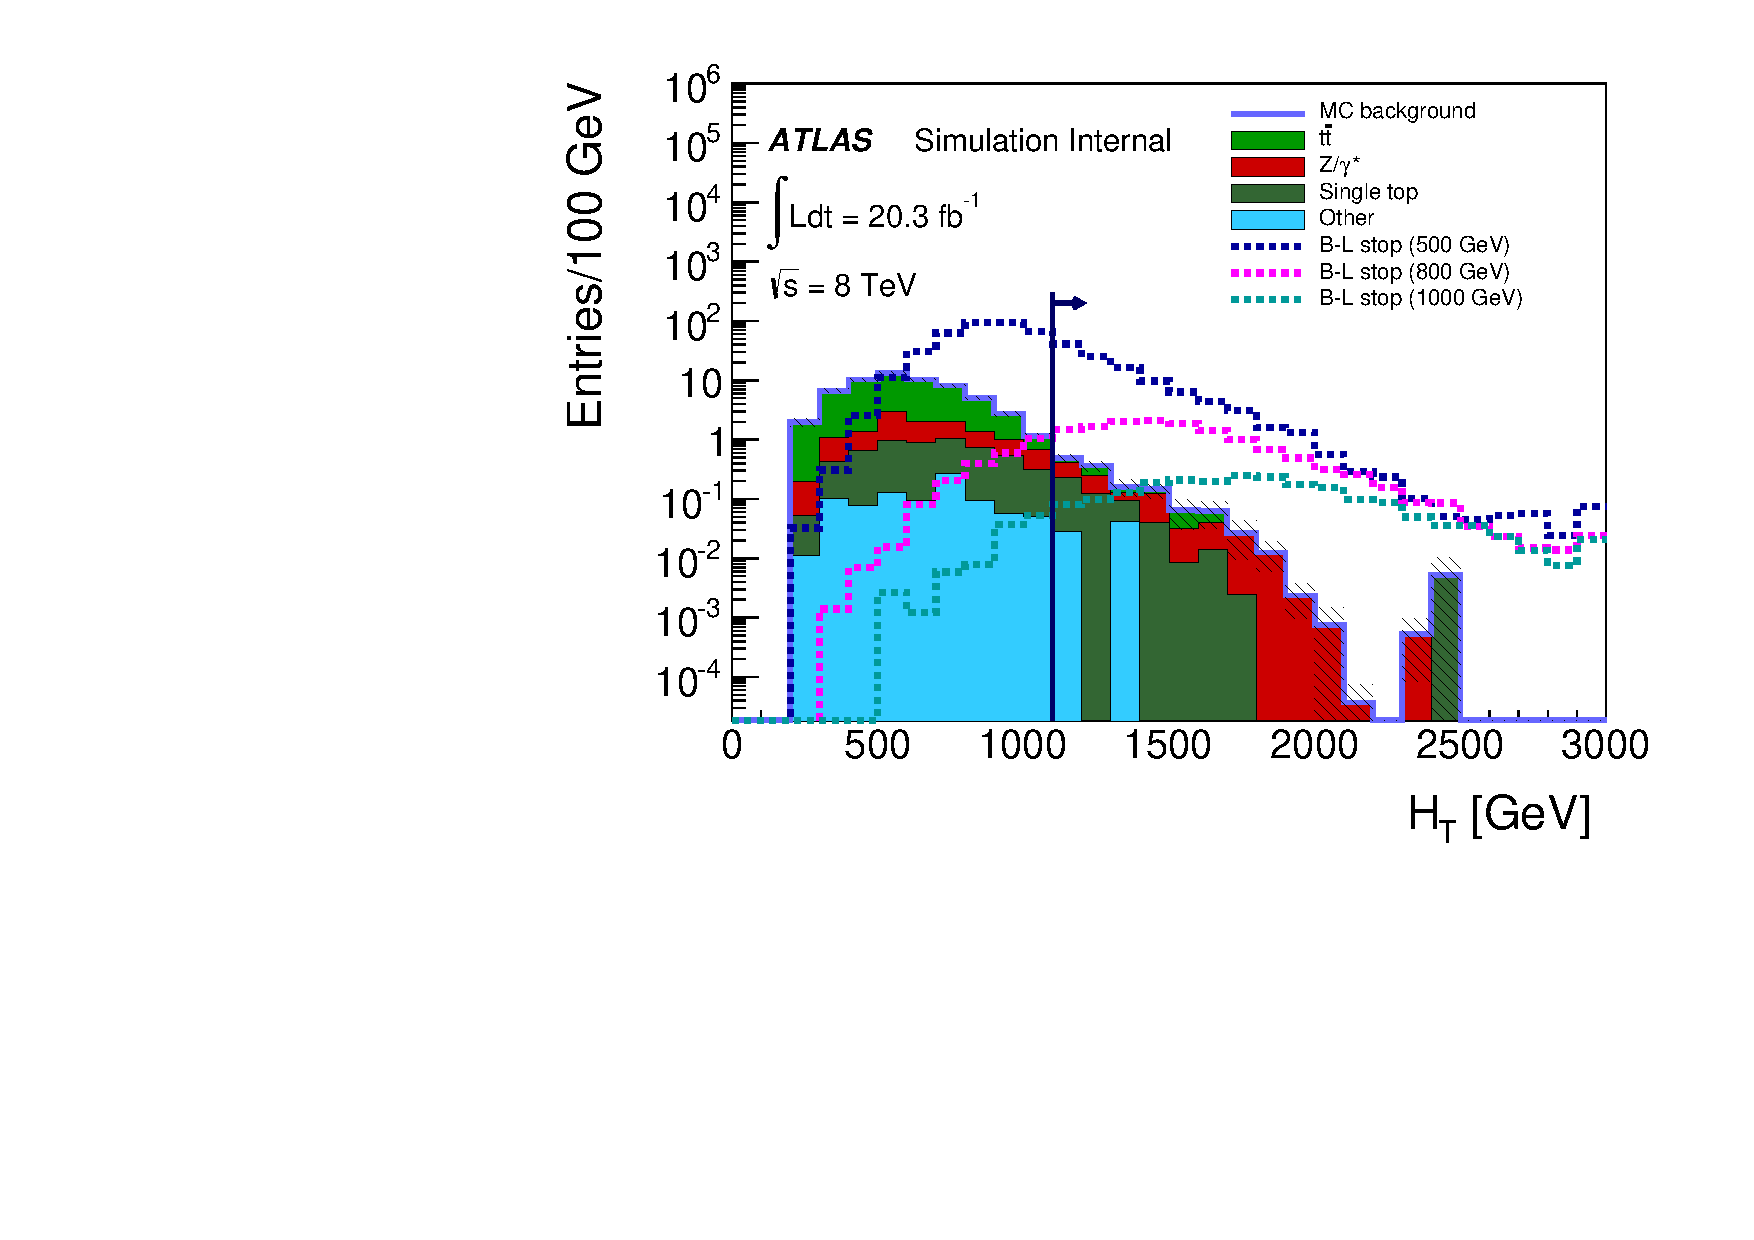
\includegraphics[width=0.9\textwidth]{figures/ht_sr_400_minus_ht.pdf}
%%% %%%     \end{block}
%%% %%%     %%
%%% %%%     \begin{block}{\MblAsym}
%%% %%%       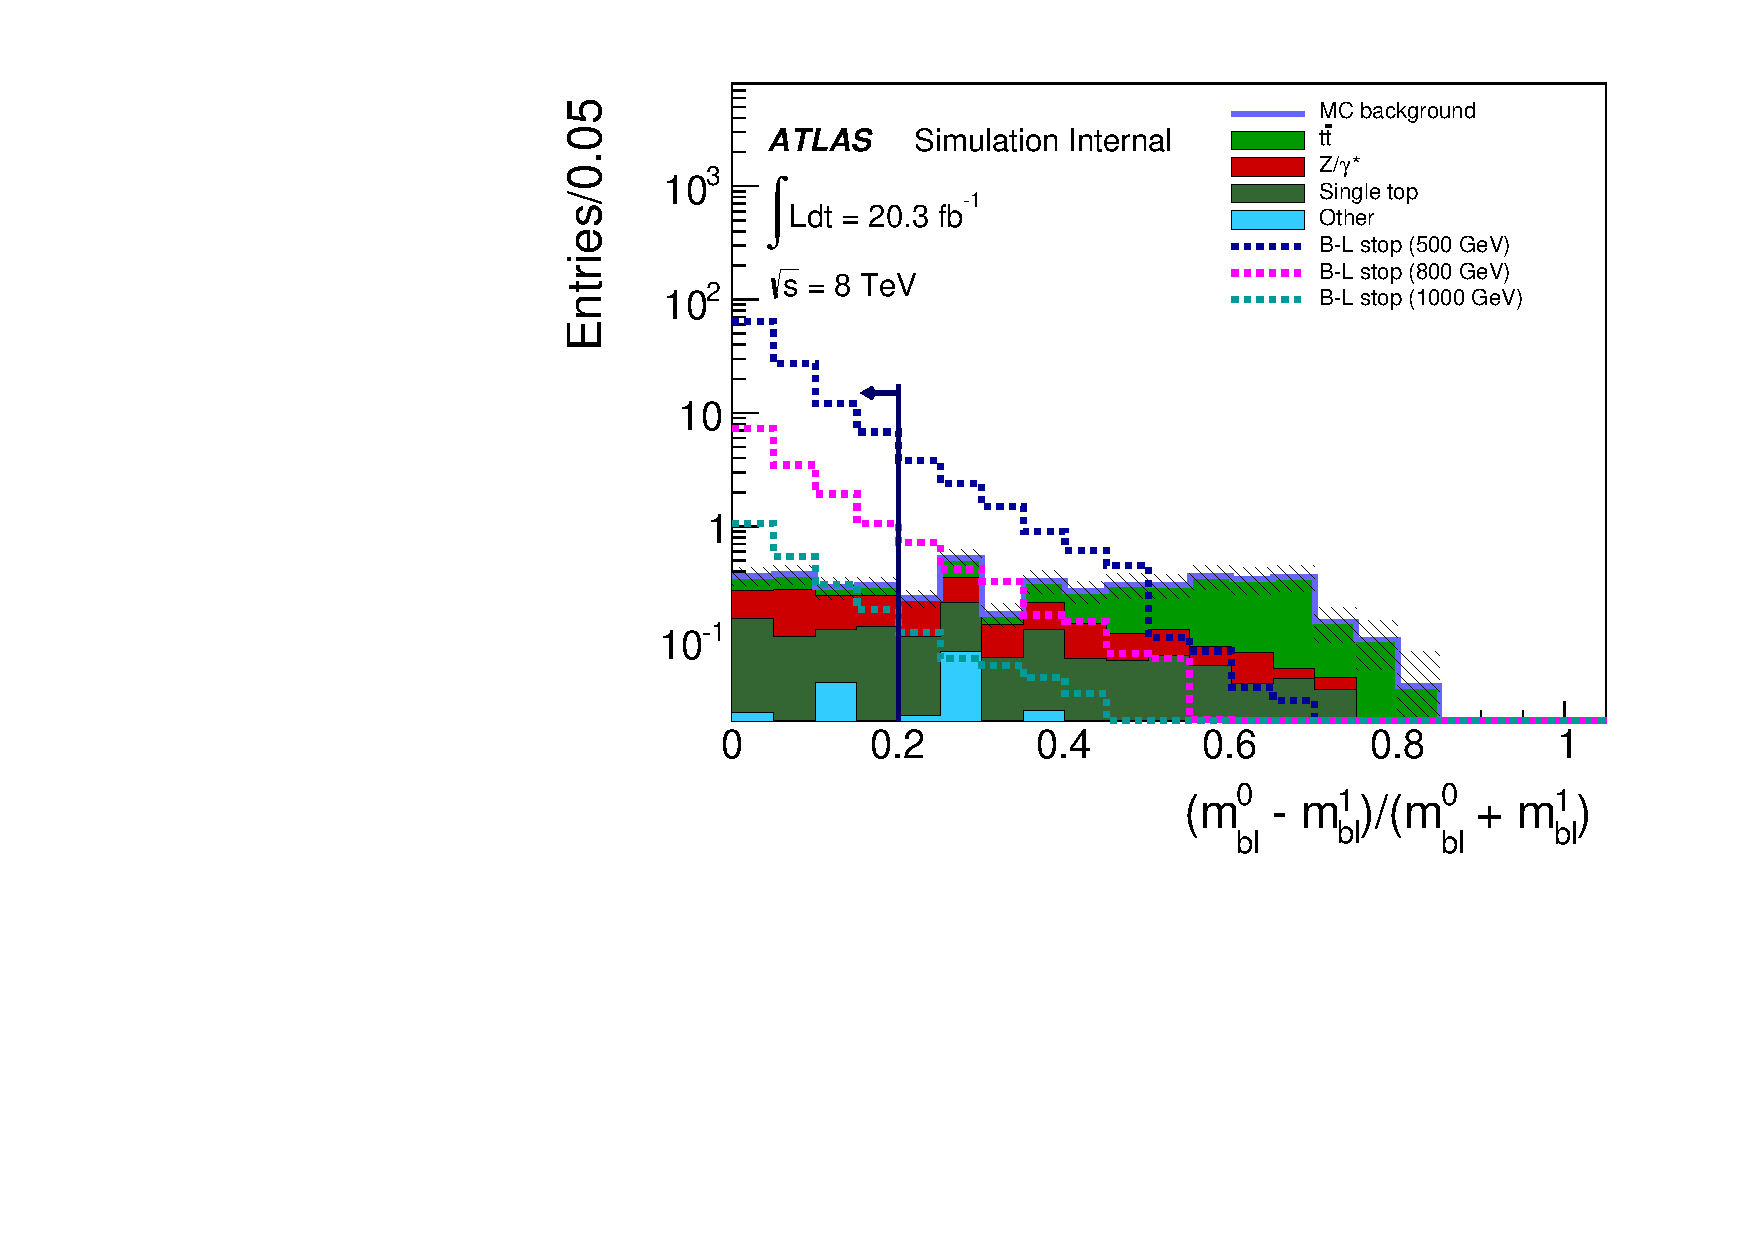
\includegraphics[width=0.9\textwidth]{figures/mbl_asym_sr_400_minus_mbl_asym.pdf}
%%% %%%     \end{block}
%%% %%%     %%
%%% %%%     \column{0.50\textwidth}
%%% %%%     \begin{block}{$\Mbl^0$}
%%% %%%       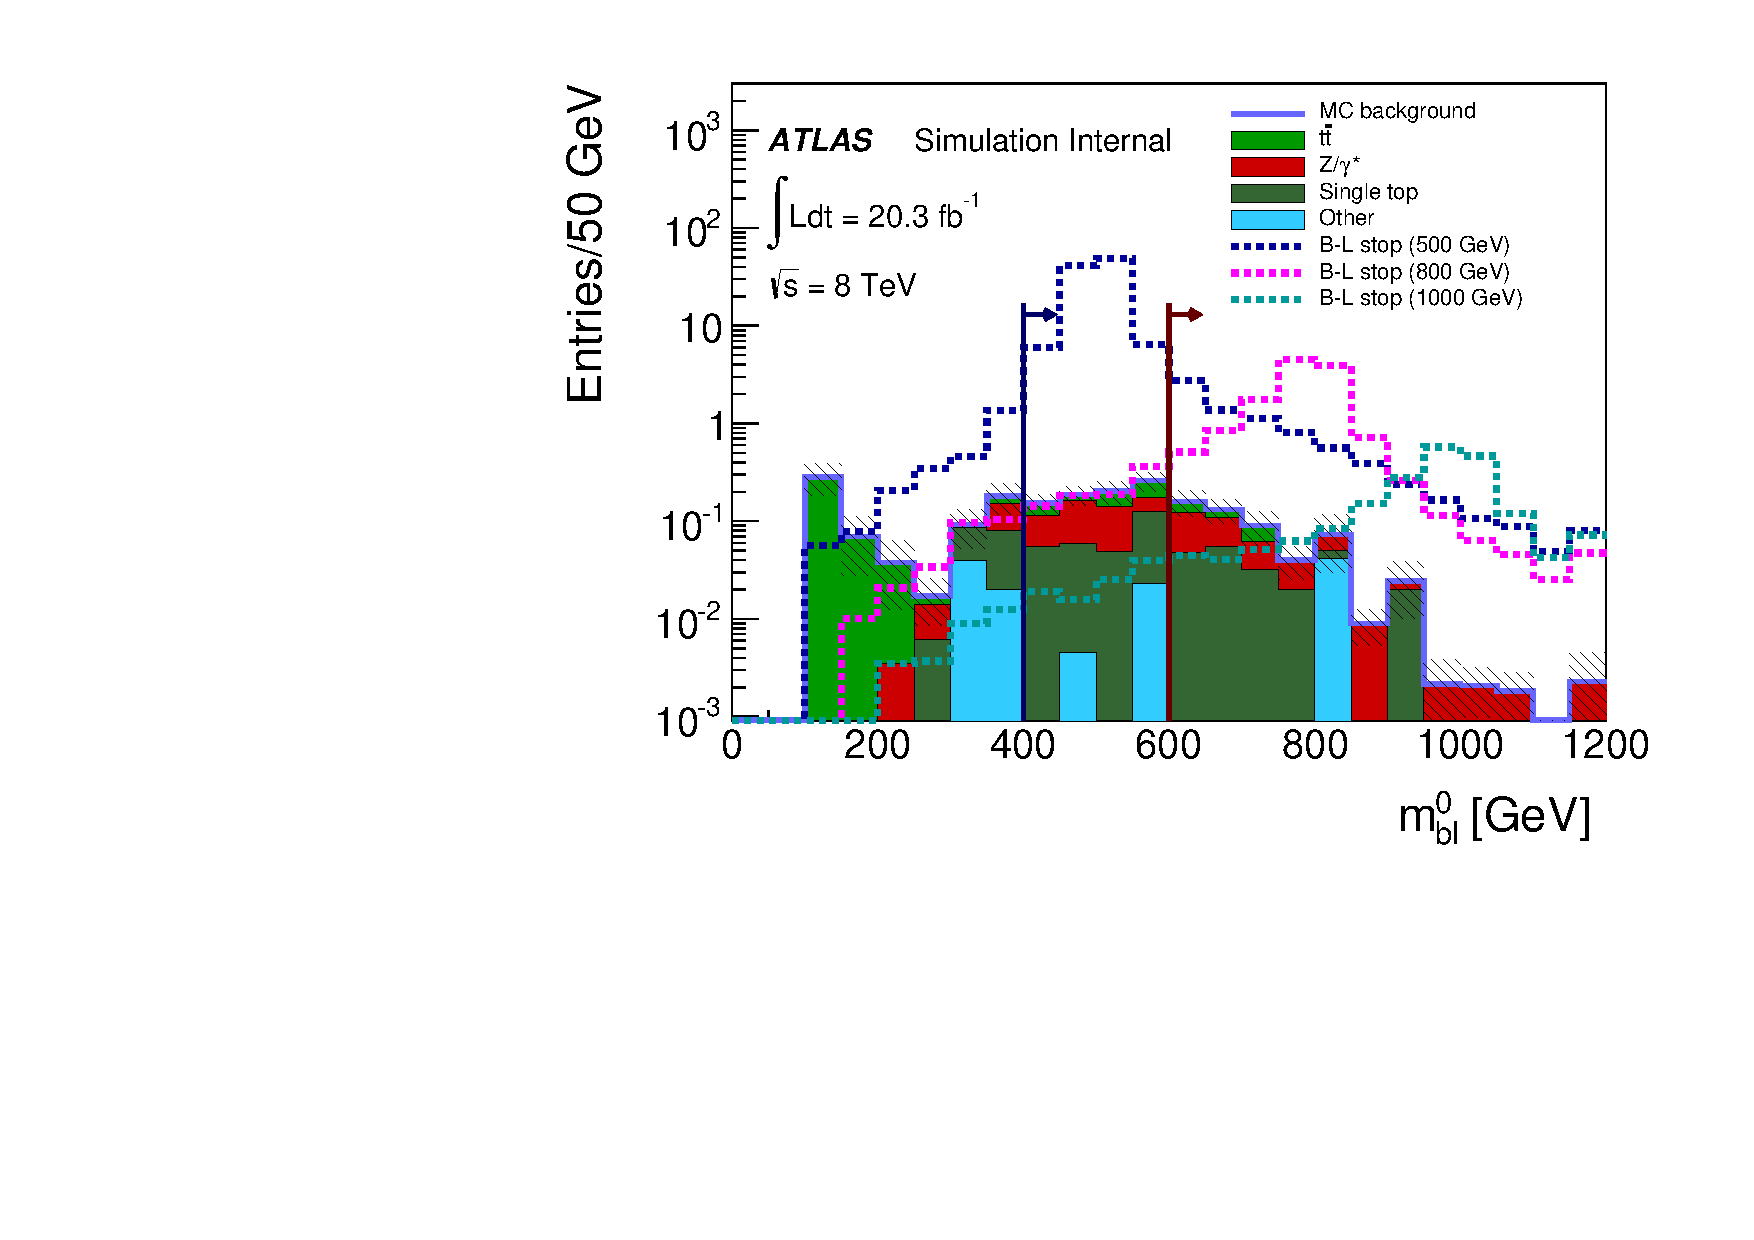
\includegraphics[width=0.9\textwidth]{figures/mbl_0_sr_minus_mbl.pdf}
%%% %%%     \end{block}
%%% %%%     %%
%%% %%%     \begin{itemize}
%%% %%%       \item Expected distributions when applying all but one of the signal
%%% %%%         region cuts
%%% %%%       \item \Ht\ and \MblAsym\ plots apply a cut of $\Mbl \ge 400$
%%% %%%     \end{itemize}
%%% %%%   \end{columns}
%%% %%% \end{frame}
%%% %%% 
%%% %%% 
%%% %%% % ------------------------------------------------------------------------------
%%% %%% \begin{frame}
%%% %%%   \frametitle{Systematic uncertainties}
%%% %%%   \begin{itemize}
%%% %%%     \item Jet energy scale: 16 parameter JES uncertainty
%%% %%%     \item B-tag scale factor uncertainty: 3 parameter uncertainty corresponding
%%% %%%       to b-jets, c-jets, and light flavor jets
%%% %%%     \item Jet energy resolution
%%% %%%     \item \Ht\ extrapolation: Additional 50\% uncertainty on the \ZGAMMA\ background
%%% %%%       in the high \Ht\ region due to disagreement in Z VR 3
%%% %%%     \item \TTBAR\ theory uncertainties
%%% %%%       \begin{itemize}
%%% %%%         \item Scale variations, MC generator,
%%% %%%           Parton Shower, ISR/FSR
%%% %%%       \end{itemize}
%%% %%%   % ----------------------------------------------------------------------------
%%% %%%   \item Single top theory uncertainties
%%% %%%     \begin{itemize}
%%% %%%       \item Cross section uncertainty, MC generator, Parton Shower,
%%% %%%         Interference with ttbar, ISR/FSR
%%% %%%     \end{itemize}
%%% %%%   % ----------------------------------------------------------------------------
%%% %%%   \item \ZGAMMA\ theory uncertainties
%%% %%%     \begin{itemize}
%%% %%%       \item Finite number of partons:
%%% %%%     \end{itemize}
%%% %%%   \item Signal cross section uncertainties are taken from
%%% %%%     {\color{blue}
%%% %%%     \href{https://twiki.cern.ch/twiki/bin/view/LHCPhysics/SUSYCrossSections8TeVstopsbottom}{SUSYCrossSections8TeVstopsbottom}}
%%% %%%   \end{itemize}
%%% %%% \end{frame}
%%% %%% 
%%% %%% 
%%% %%% % ------------------------------------------------------------------------------
%%% %%% \begin{frame}
%%% %%%   \frametitle{Systematic uncertainty breakdown}
%%% %%% 
%%% %%%   \begin{columns}
%%% %%%     \column{0.5\linewidth}
%%% %%%     \begin{block}{SR 400}
%%% %%%       \vspace{1ex}
%%% %%%       \resizebox{\linewidth}{!}{
%%% %%%         \begin{tabular}{l|cccc|c}
%%% %%%           \toprule
%%% %%%           Systematic                   & $t\bar{t}$ & $Z/\gamma^{*}$ & Single top & Other   & Total   \\
%%% %%%           \midrule
%%% %%%           Uncertainty (\%)                                                                            \\
%%% %%%           \midrule
%%% %%%           JES                          & +58/-0     & +1/-12         & +4/-4      & +5/-91  & +15/-11 \\
%%% %%%           $b$-tagging                  & +14/-13    & +15/-14        & +11/-10    & +12/-11 & +13/-12 \\
%%% %%%           JER                          & 25         & 2              & 2          & 0       & 7       \\
%%% %%%           Luminosity                   & -          & -              & 2          & 2       & 1       \\
%%% %%%           \midrule
%%% %%%           \Ht\ extrapolation           & -          & 50             & -          & -       & 19      \\
%%% %%%           MC Statistical               & 25         & 4              & 10         & 50      & 13      \\
%%% %%%           CR Statistical               & 5          & 5              & -          & -       & 3       \\
%%% %%%           $Wt$ cross section           & -          & -              & 7          & -       & 2       \\
%%% %%%           Renormalization Scale        & 6          & -              & -          & -       & 1       \\
%%% %%%           Parton shower                & 0          & -              & -          & -       & 0       \\
%%% %%%           Multi-parton                 & -          & 0              & -          & -       & 0       \\
%%% %%%           ISR/FSR                      & 2          & -              & 0          & -       & 0       \\
%%% %%%           Factorization Scale          & 1          & -              & -          & -       & 0       \\
%%% %%%           Interference with $t\bar{t}$ & -          & -              & 0          & -       & 0       \\
%%% %%%           \bottomrule
%%% %%%         \end{tabular}
%%% %%%       }
%%% %%%     \end{block}
%%% %%%     %%
%%% %%%     \column{0.5\linewidth}
%%% %%%     \begin{block}{SR 600}
%%% %%%       \vspace{1ex}
%%% %%%       \resizebox{\linewidth}{!}{
%%% %%%         \begin{tabular}{l|cccc|c}
%%% %%%           \toprule
%%% %%%           Systematic                   & $t\bar{t}$ & $Z/\gamma^{*}$ & Single top & Other   & Total   \\
%%% %%%           \midrule
%%% %%%           Uncertainty (\%)                                                                            \\
%%% %%%           \midrule
%%% %%%           JES                          & +0/-0      & +1/-4          & +6/-0      & +10/-0  & +3/-2   \\
%%% %%%           $b$-tagging                  & +12/-11    & +12/-11        & +12/-11    & +11/-10 & +12/-11 \\
%%% %%%           JER                          & 0          & 3              & 0          & 0       & 1       \\
%%% %%%           Luminosity                   & -          & -              & 2          & 2       & 1       \\
%%% %%%           \midrule
%%% %%%           \Ht\ extrapolation           & -          & 50             & -          & -       & 20      \\
%%% %%%           MC Statistical               & 57         & 6              & 17         & 70      & 23      \\
%%% %%%           CR Statistical               & 5          & 5              & -          & -       & 3       \\
%%% %%%           $Wt$ cross section           & -          & -              & 7          & -       & 2       \\
%%% %%%           Renormalization Scale        & 0          & -              & -          & -       & 0       \\
%%% %%%           Parton shower                & 0          & -              & -          & -       & 0       \\
%%% %%%           Multi-parton                 & -          & 0              & -          & -       & 0       \\
%%% %%%           ISR/FSR                      & 0          & -              & 0          & -       & 0       \\
%%% %%%           Factorization Scale          & 16         & -              & -          & -       & 2       \\
%%% %%%           Interference with $t\bar{t}$ & -          & -              & 0          & -       & 0       \\
%%% %%%           \bottomrule
%%% %%%         \end{tabular}
%%% %%%       }
%%% %%%     \end{block}
%%% %%%   \end{columns}
%%% %%% \end{frame}
%%% %%% 
%%% %%% 
%%% %%% % ------------------------------------------------------------------------------
%%% %%% \begin{frame}
%%% %%%   \frametitle{Background estimate - control regions}
%%% %%%   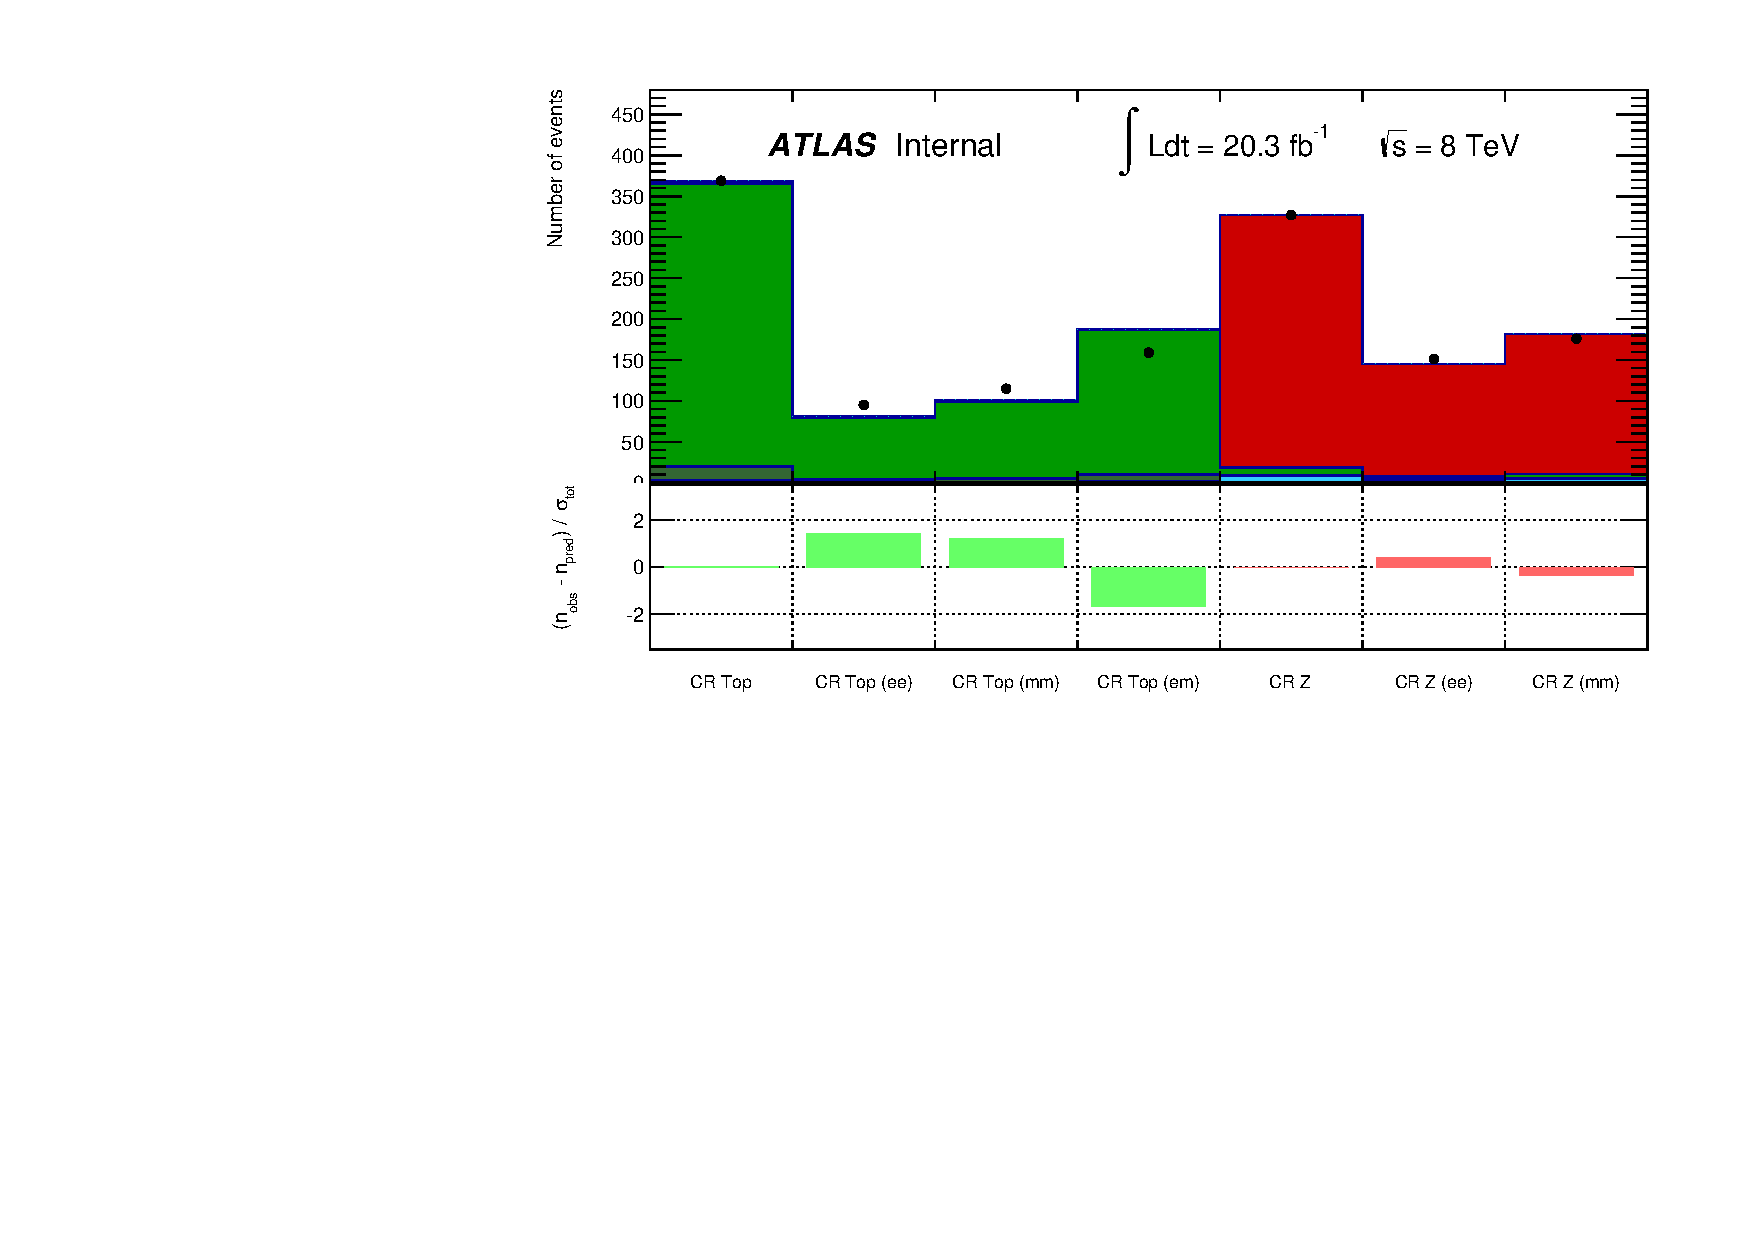
\includegraphics[width=\textwidth]{figures/histpull_CR_detailed.pdf}
%%% %%%   \begin{itemize}
%%% %%%     \item \TTBAR\ and \ZGAMMA\ normalizations were constrained using a fit to
%%% %%%       the observed data in the control regions
%%% %%%     \item Systematics included as Gaussian nuissance parameters
%%% %%%     \item {\color{blue}\textbf{Postfit normalization in the control
%%% %%%       regions is fairly good}}
%%% %%%   \end{itemize}
%%% %%% \end{frame}
%%% %%% 
%%% %%% 
%%% %%% % ------------------------------------------------------------------------------
%%% %%% \begin{frame}
%%% %%%   \frametitle{Top control region}
%%% %%%   %%
%%% %%%   \begin{columns}
%%% %%%     \column{0.45\textwidth}
%%% %%%     \begin{block}{\Ht}
%%% %%%       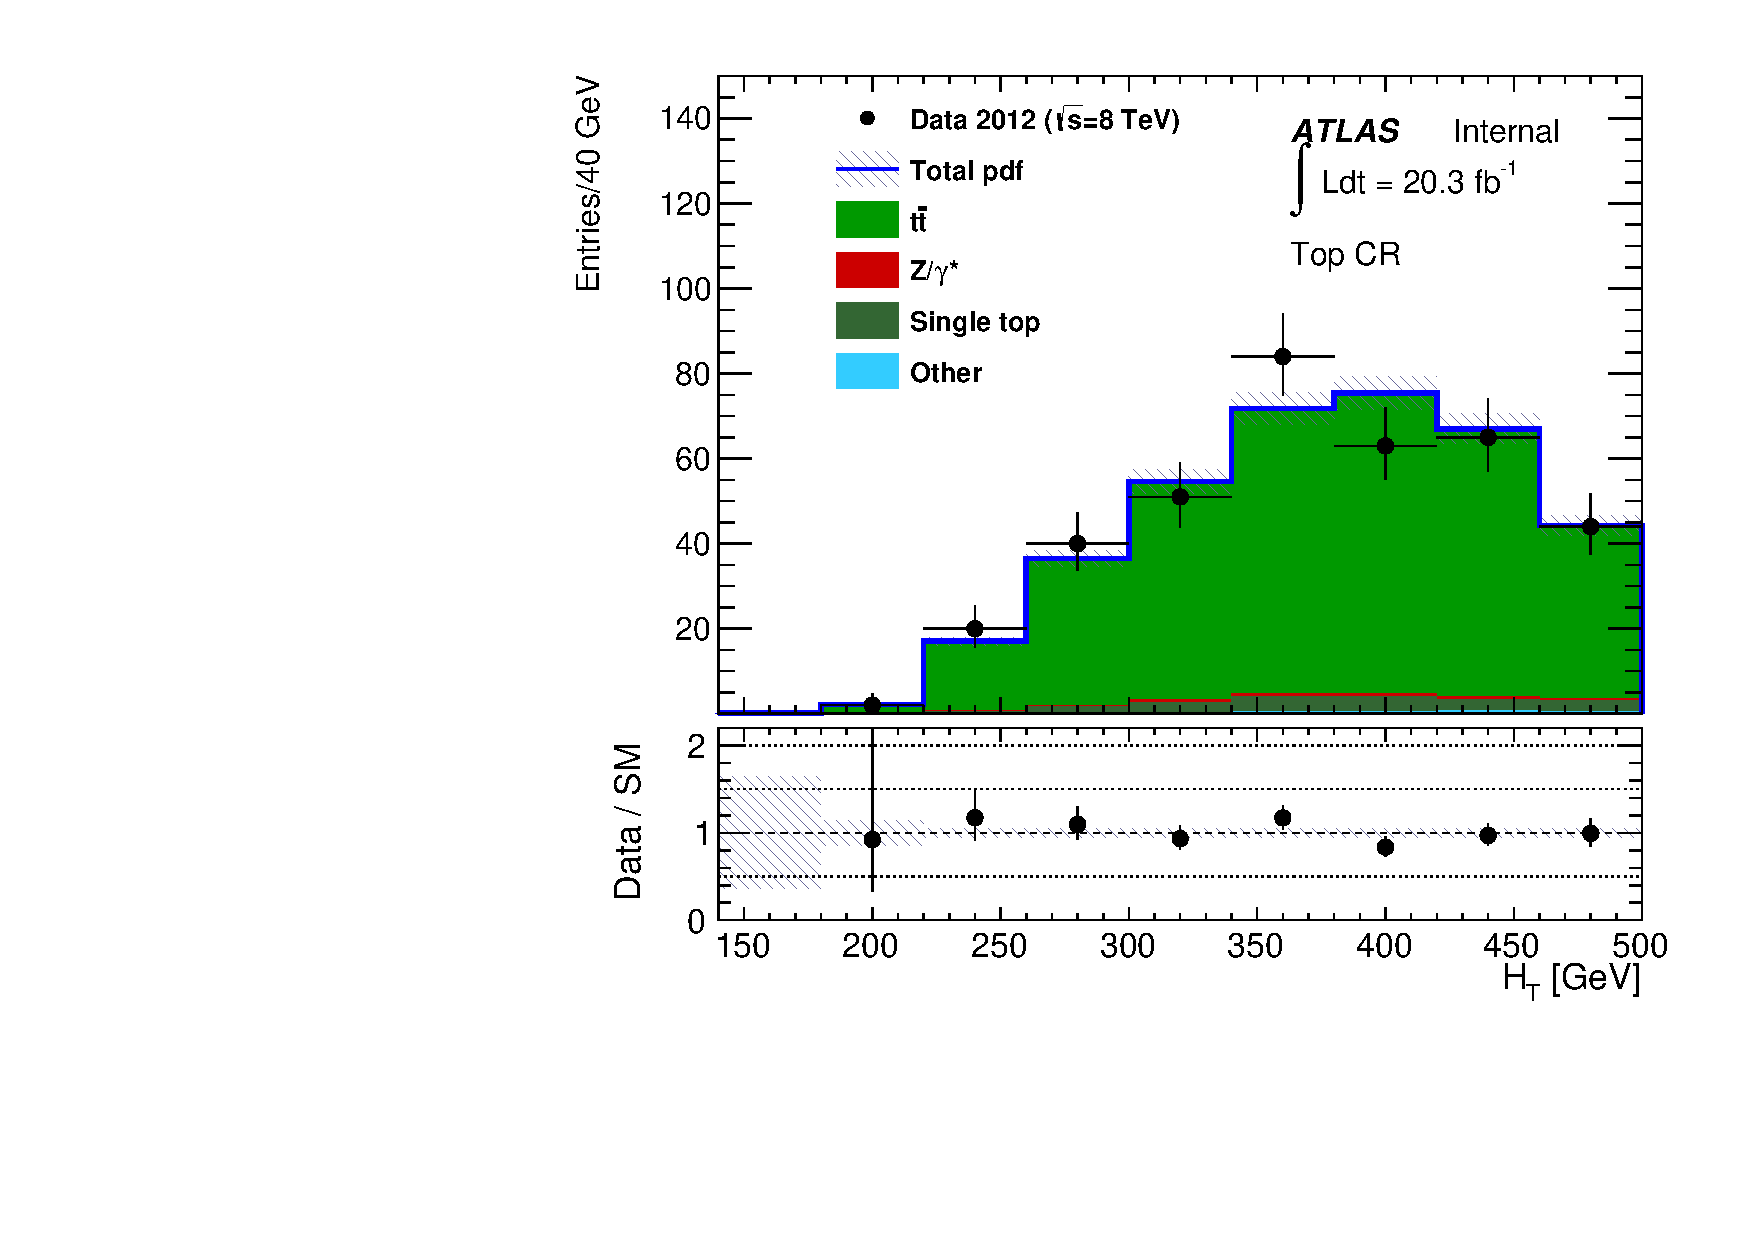
\includegraphics[width=\textwidth]{figures/cr_top_ht_signal.pdf}
%%% %%%     \end{block}
%%% %%%     \column{0.45\textwidth}
%%% %%%     \begin{block}{\Mbl}
%%% %%%       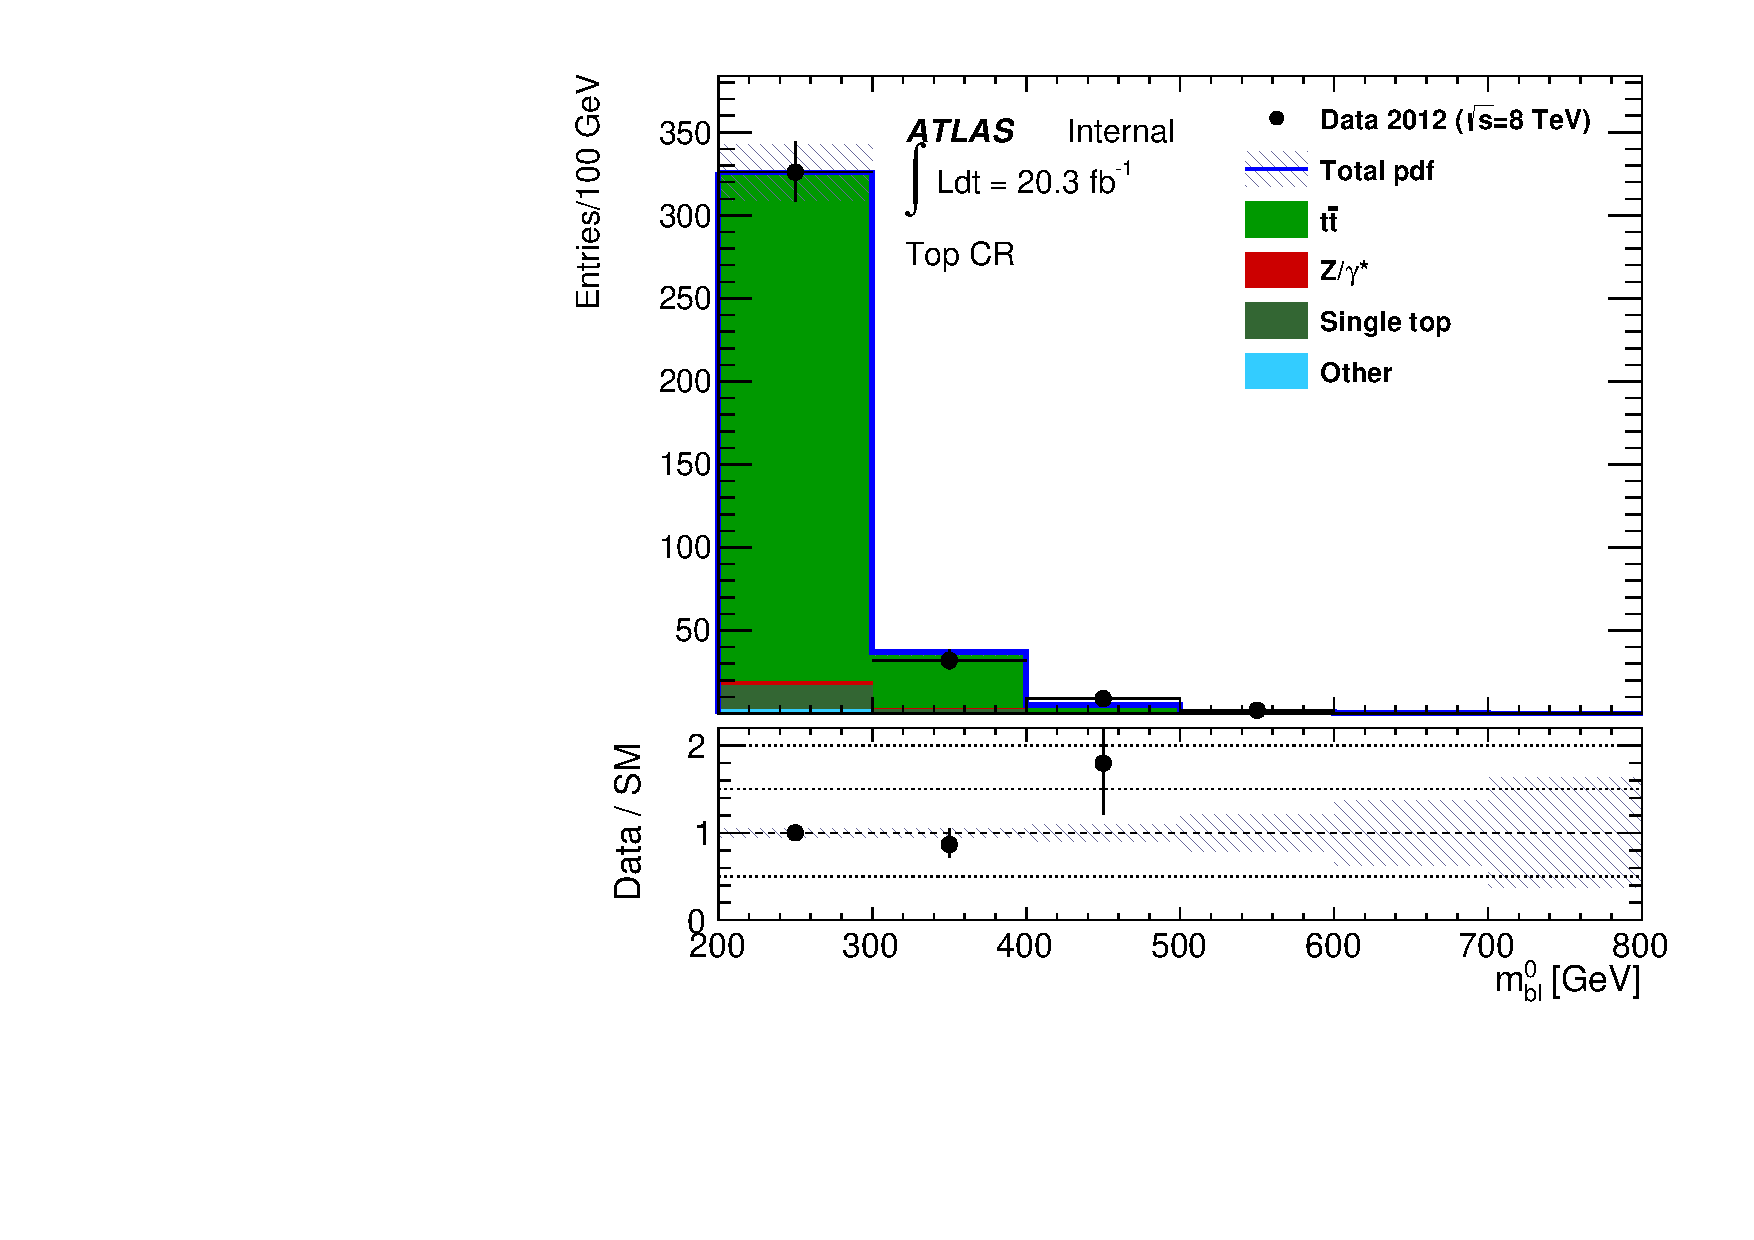
\includegraphics[width=\textwidth]{figures/cr_top_mbl_0.pdf}
%%% %%%     \end{block}
%%% %%%   \end{columns}
%%% %%%   %%
%%% %%%   \begin{itemize}
%%% %%%     \item Best fit normalization factor: $\mu_{\TTBAR} = 1.11 \pm 0.14$
%%% %%%     \item Good agreement in the top control region
%%% %%%     \item Top background seems to be well modeled
%%% %%%   \end{itemize}
%%% %%% \end{frame}
%%% %%% 
%%% %%% 
%%% %%% % ------------------------------------------------------------------------------
%%% %%% \begin{frame}
%%% %%%   \frametitle{Z control region}
%%% %%%   %%
%%% %%%   \begin{columns}
%%% %%%     \column{0.45\textwidth}
%%% %%%     \begin{block}{\Ht}
%%% %%%       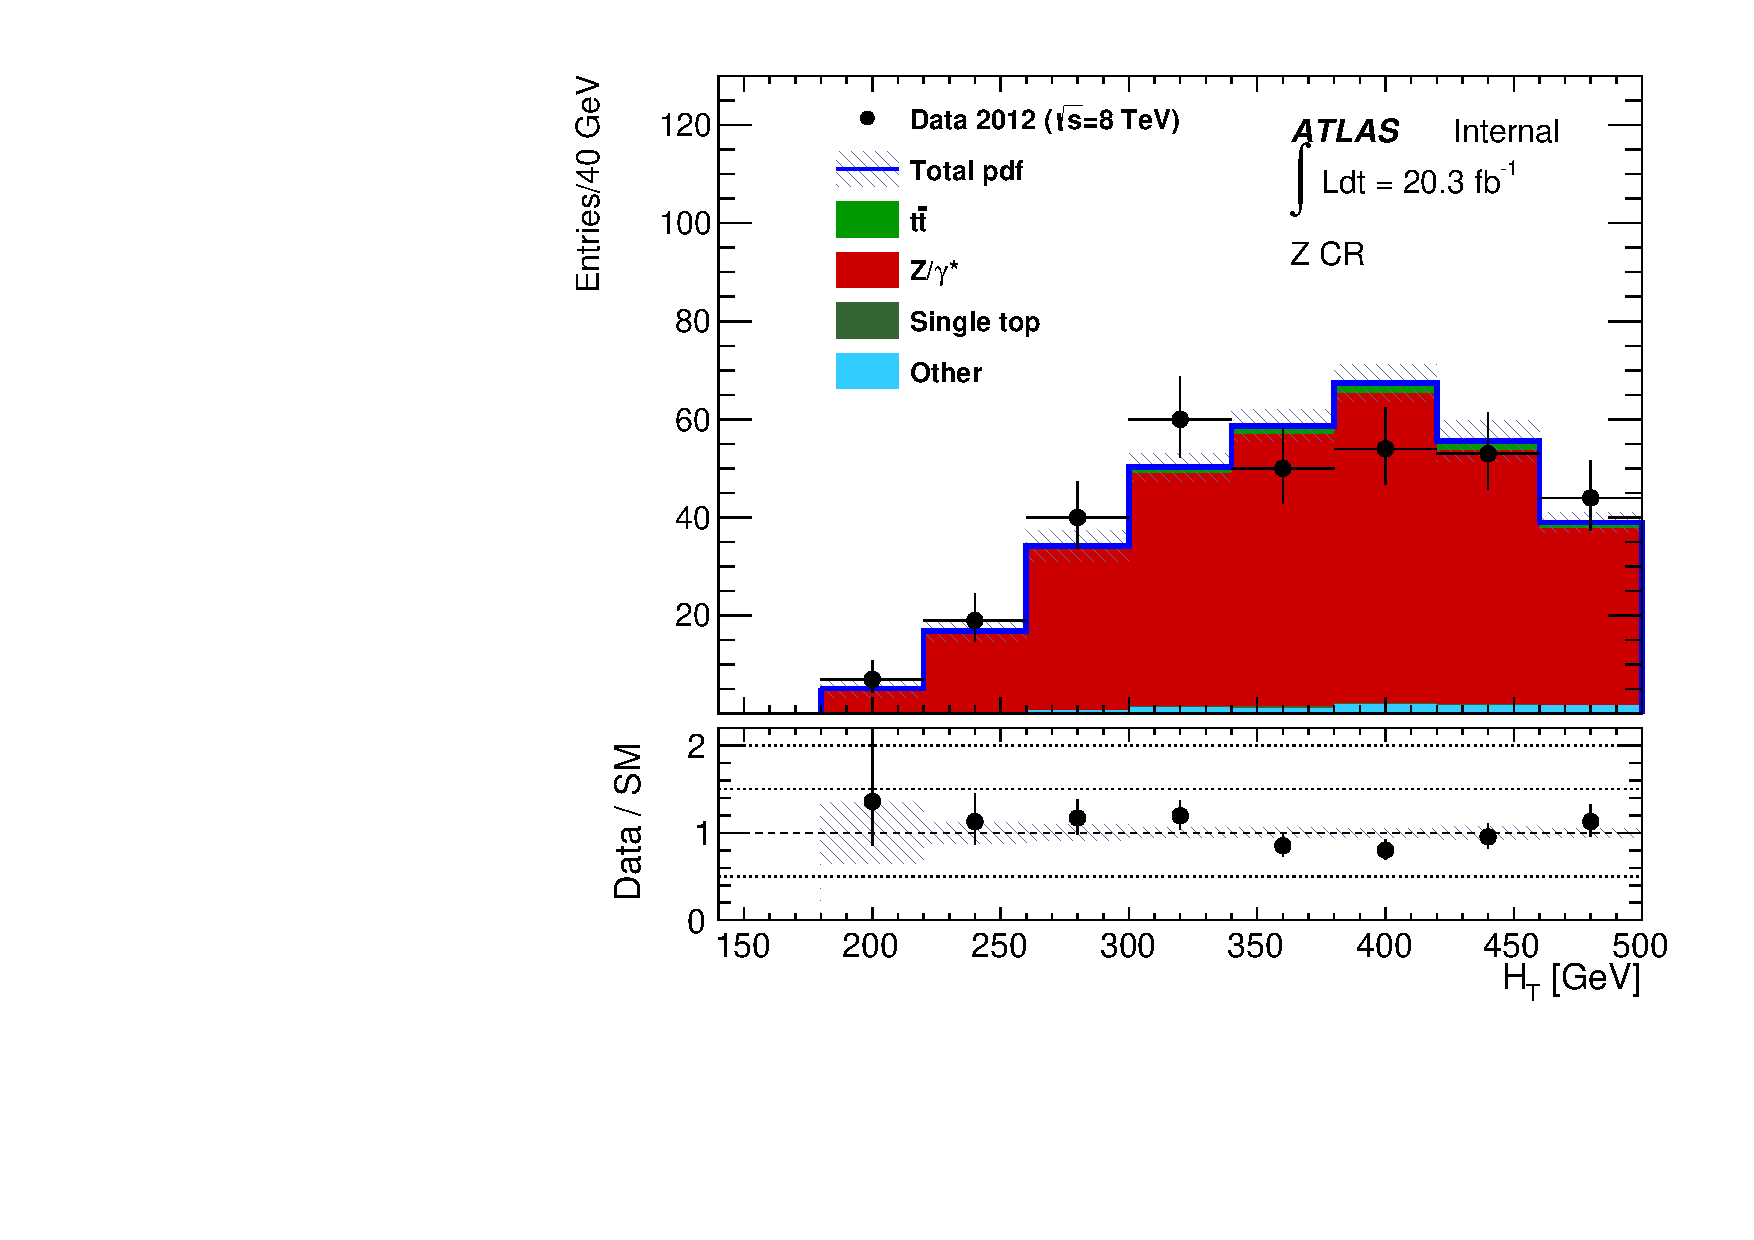
\includegraphics[width=\textwidth]{figures/cr_Z_ht_signal.pdf}
%%% %%%     \end{block}
%%% %%%     \column{0.45\textwidth}
%%% %%%     \begin{block}{\Mbl}
%%% %%%       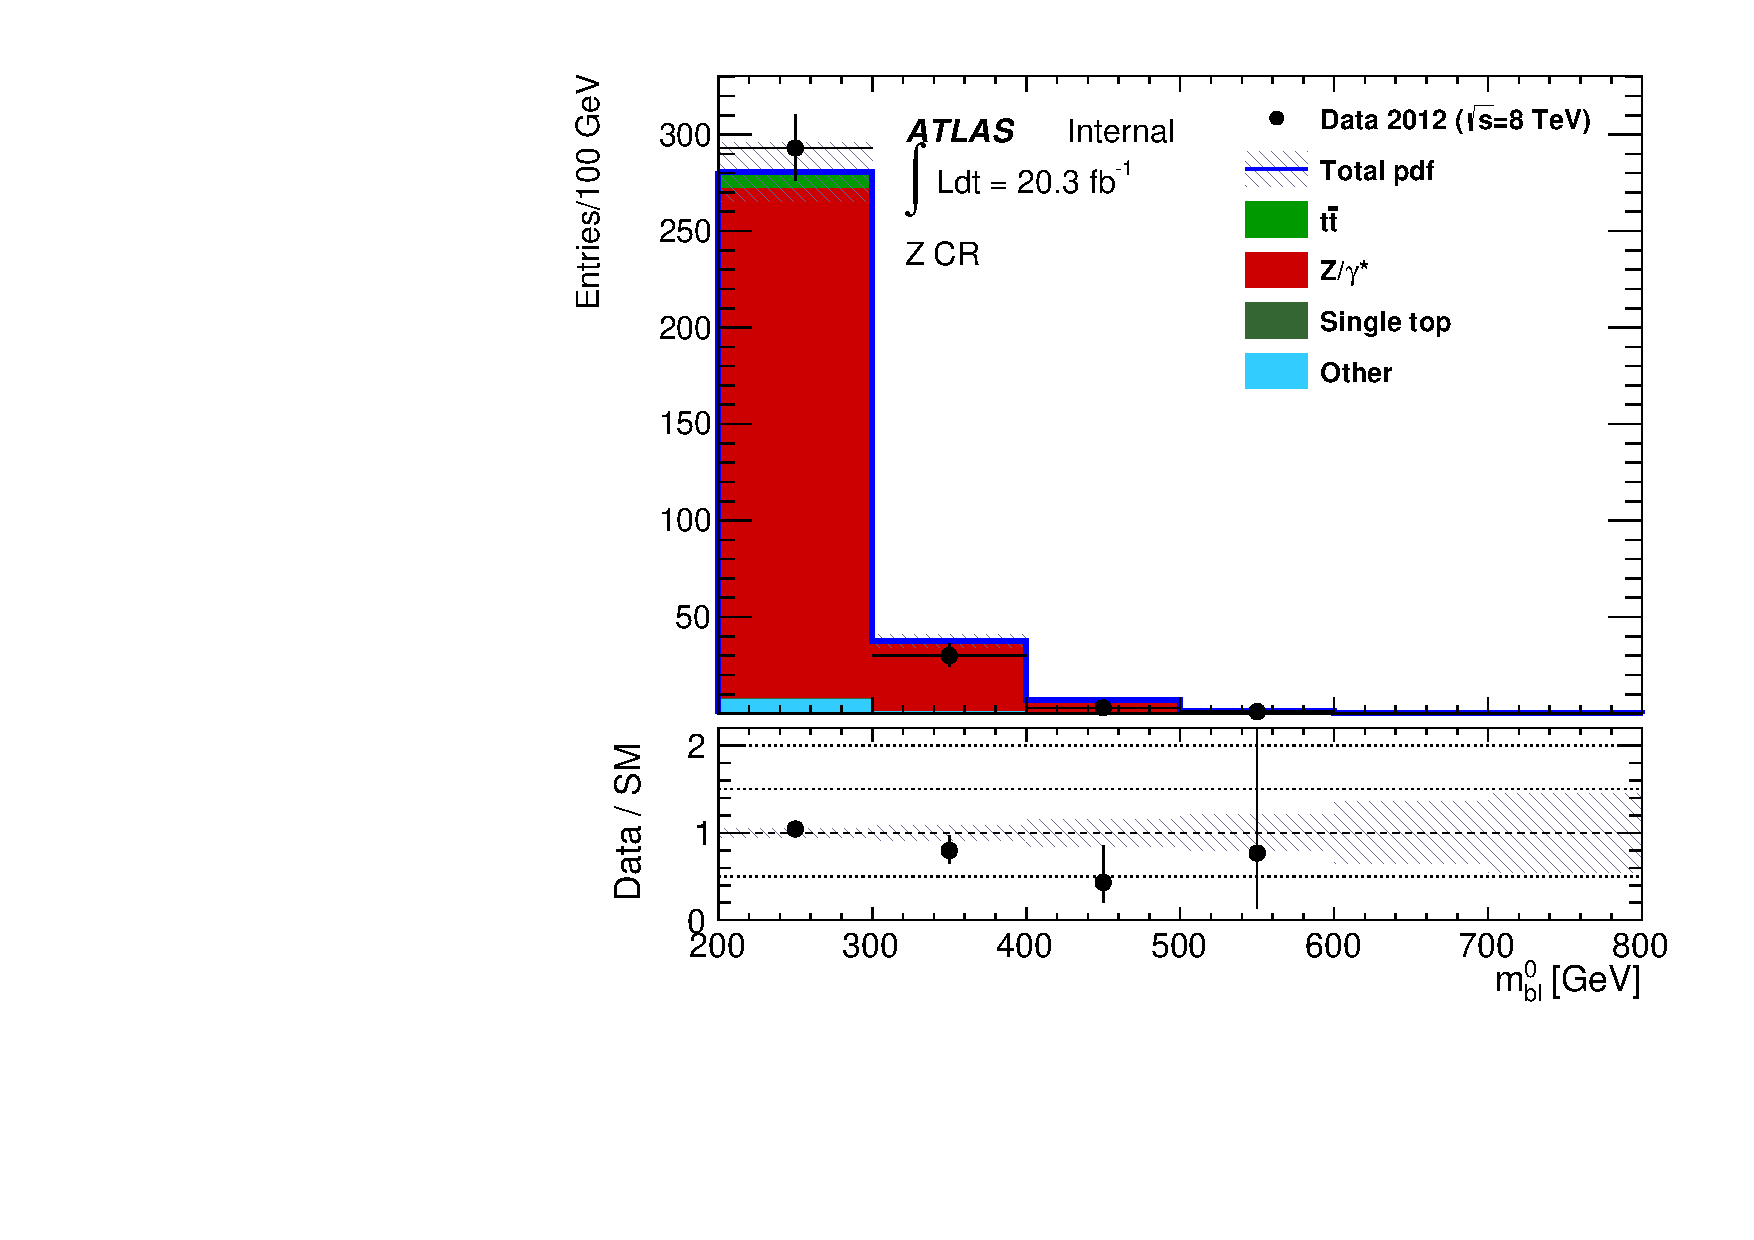
\includegraphics[width=\textwidth]{figures/cr_Z_mbl_0.pdf}
%%% %%%     \end{block}
%%% %%%   \end{columns}
%%% %%%   %%
%%% %%%   \begin{itemize}
%%% %%%     \item Best fit normalization factor: $\mu_{\ZGAMMA} = 1.43 \pm 0.19$
%%% %%%     \item Good agreement in the $Z$ control region
%%% %%%     \item Despite large normalization factor, the \ZGAMMA\ background seems
%%% %%%       well modeled in this region
%%% %%%   \end{itemize}
%%% %%% \end{frame}
%%% %%% 
%%% %%% 
%%% %%% % ------------------------------------------------------------------------------
%%% %%% \begin{frame}
%%% %%%   \frametitle{Background estimate - validation regions}
%%% %%%   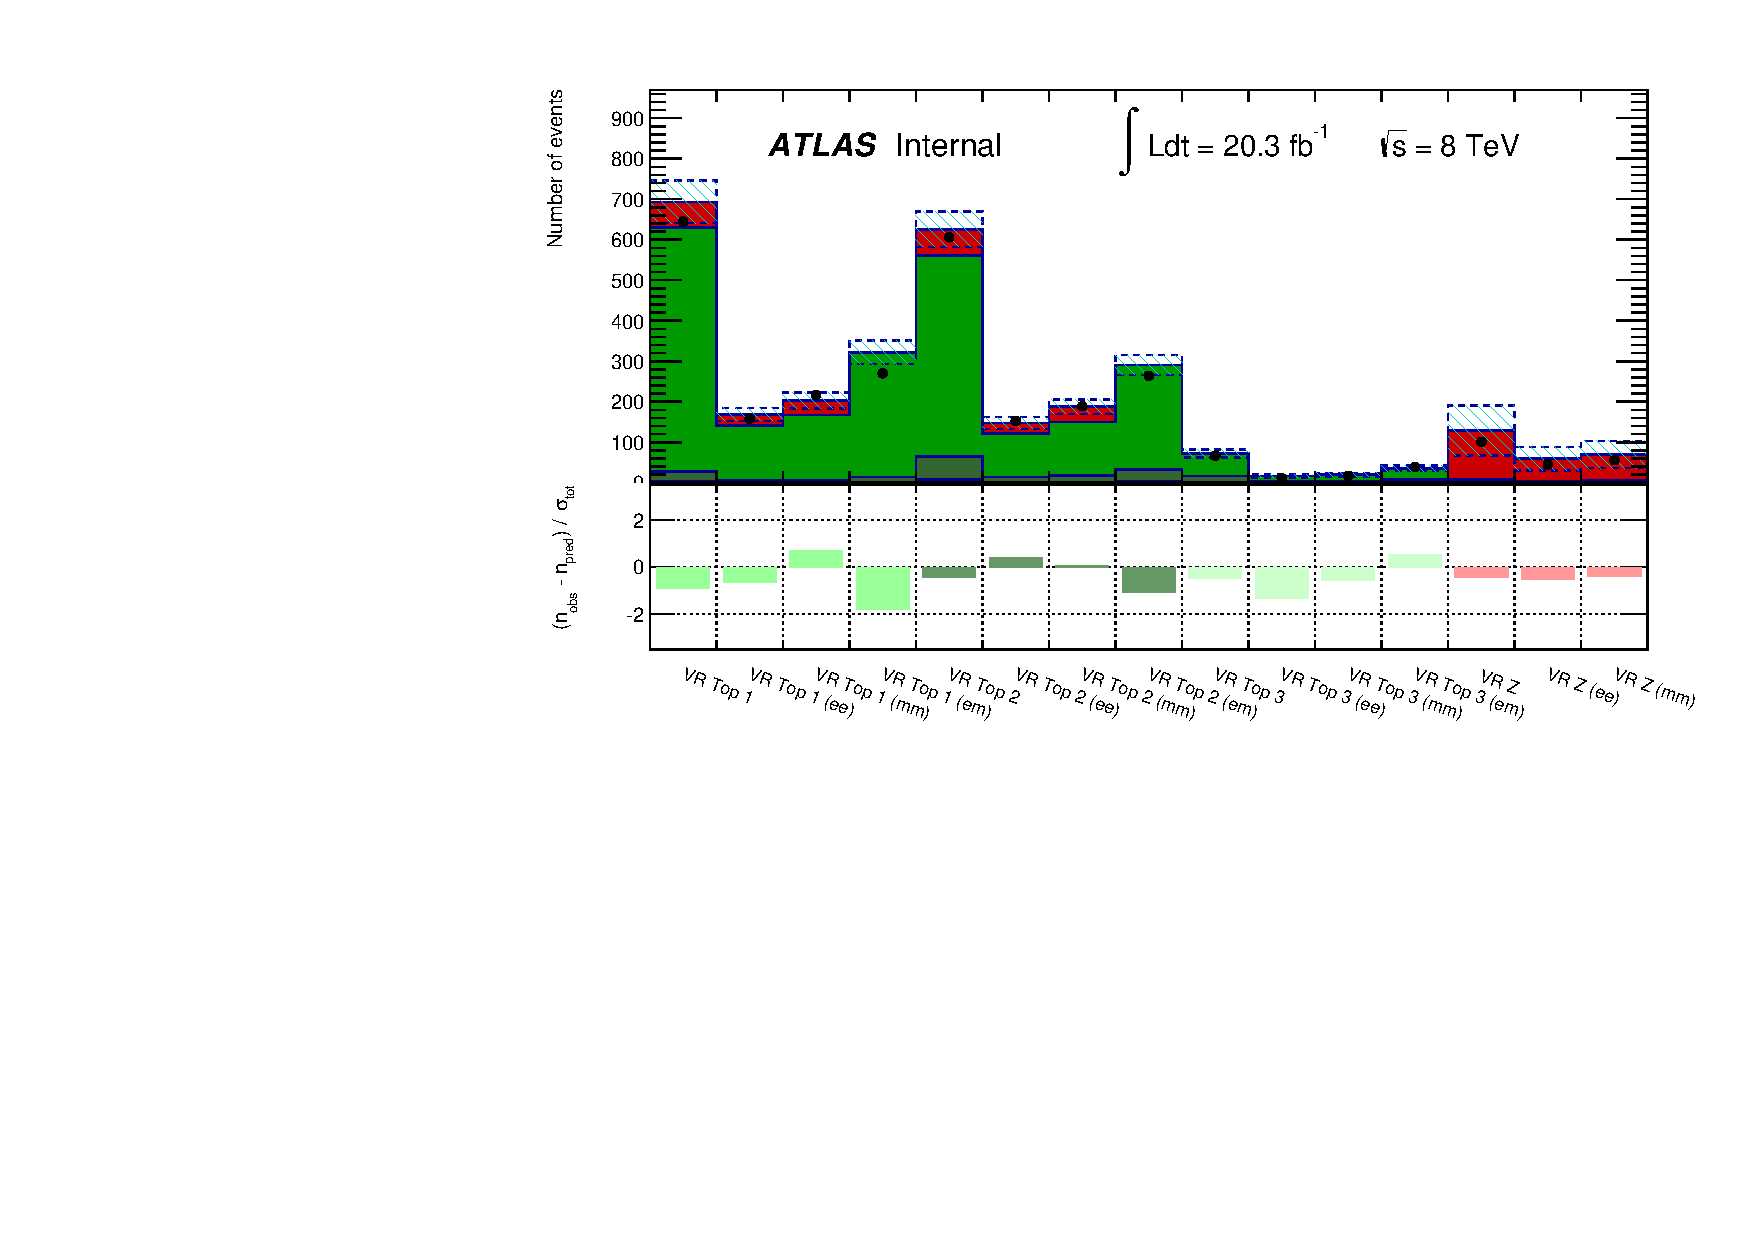
\includegraphics[width=\textwidth]{figures/histpull_VR_detailed.pdf}
%%% %%%   \begin{itemize}
%%% %%%     \item Extrapolate the fit results from the control region to the validation
%%% %%%       regions
%%% %%%     \item Overall good agreement in the validation regions
%%% %%%   \end{itemize}
%%% %%% \end{frame}
%%% %%% 
%%% %%% 
%%% %%% % ------------------------------------------------------------------------------
%%% %%% \begin{frame}
%%% %%%   \frametitle{Top validation region 3}
%%% %%%   %%
%%% %%%   \begin{columns}
%%% %%%     \column{0.45\textwidth}
%%% %%%     \begin{block}{\Ht}
%%% %%%       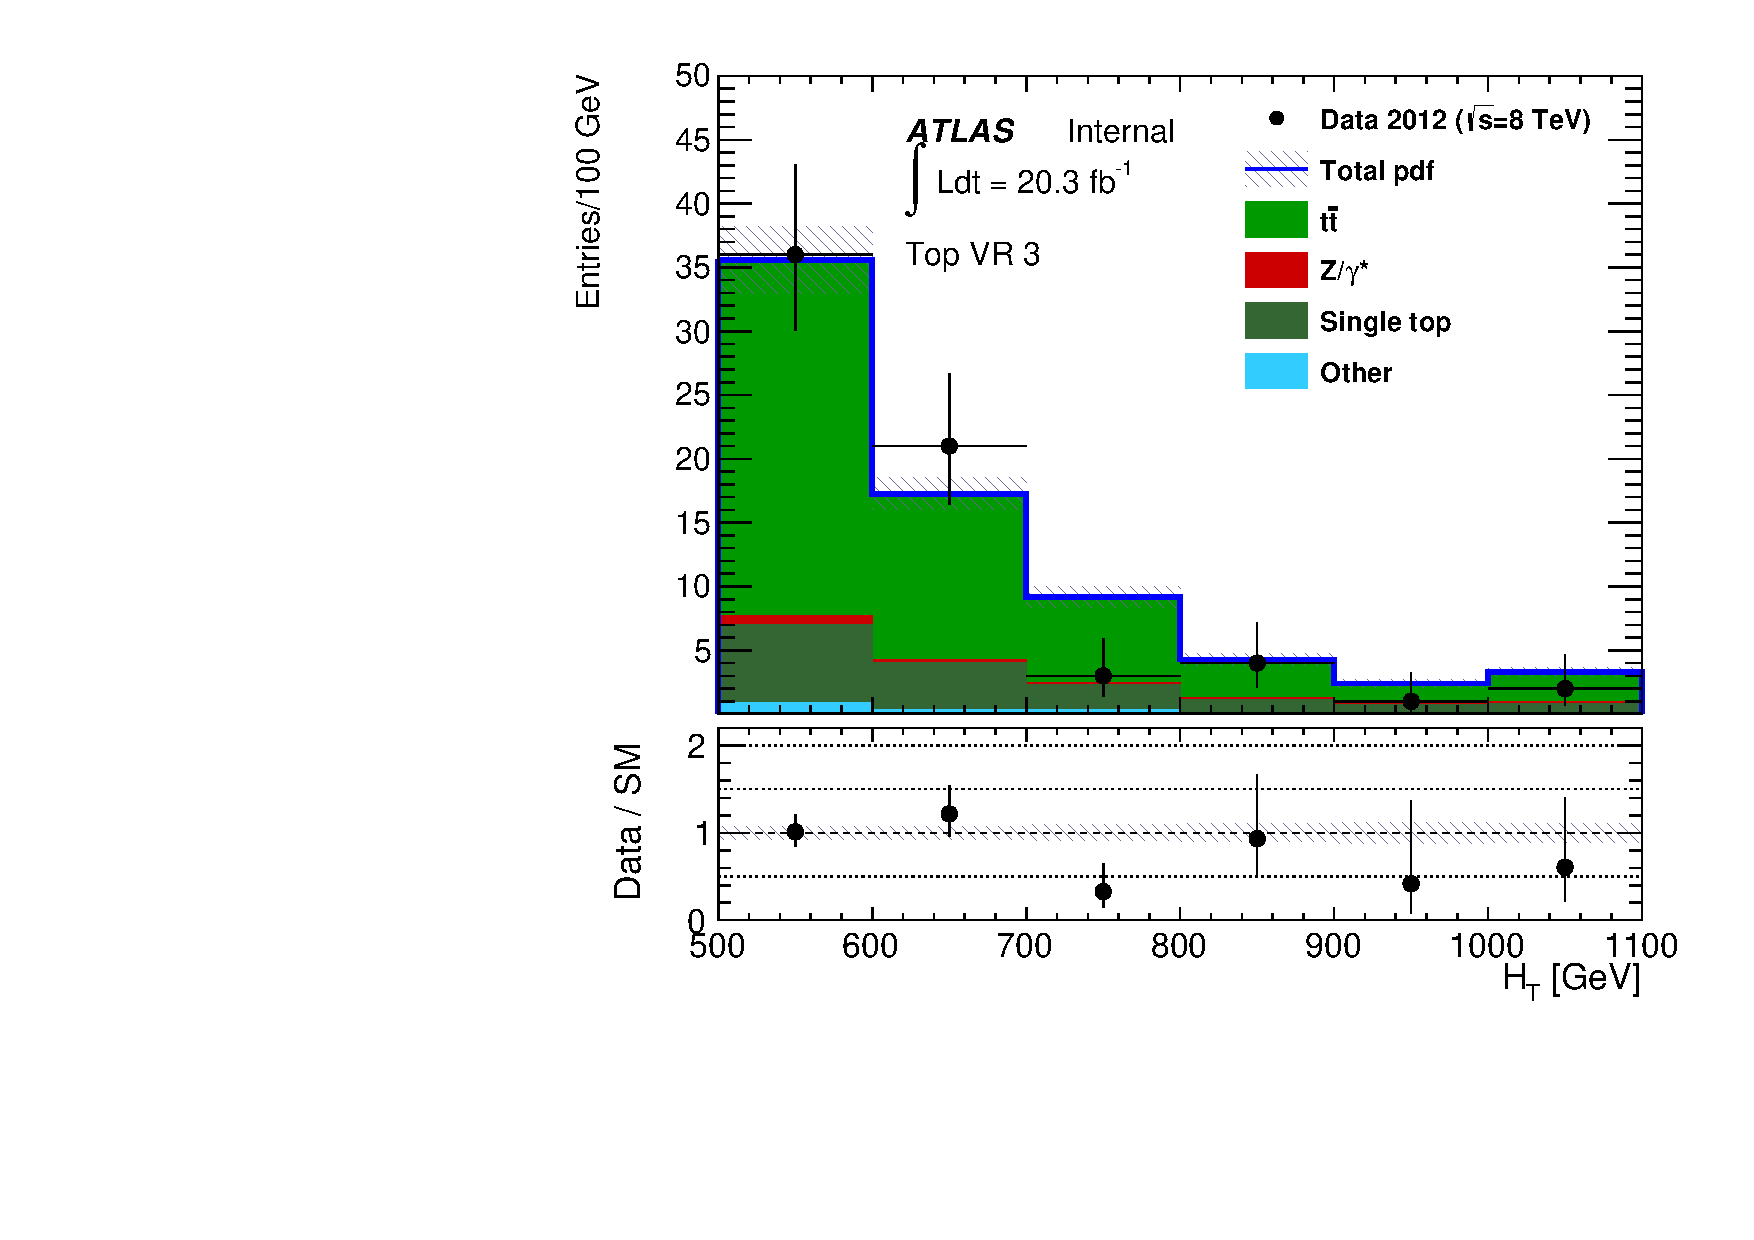
\includegraphics[width=\textwidth]{figures/vr_top_3_ht_signal.pdf}
%%% %%%     \end{block}
%%% %%%     \column{0.45\textwidth}
%%% %%%     \begin{block}{\Mbl}
%%% %%%       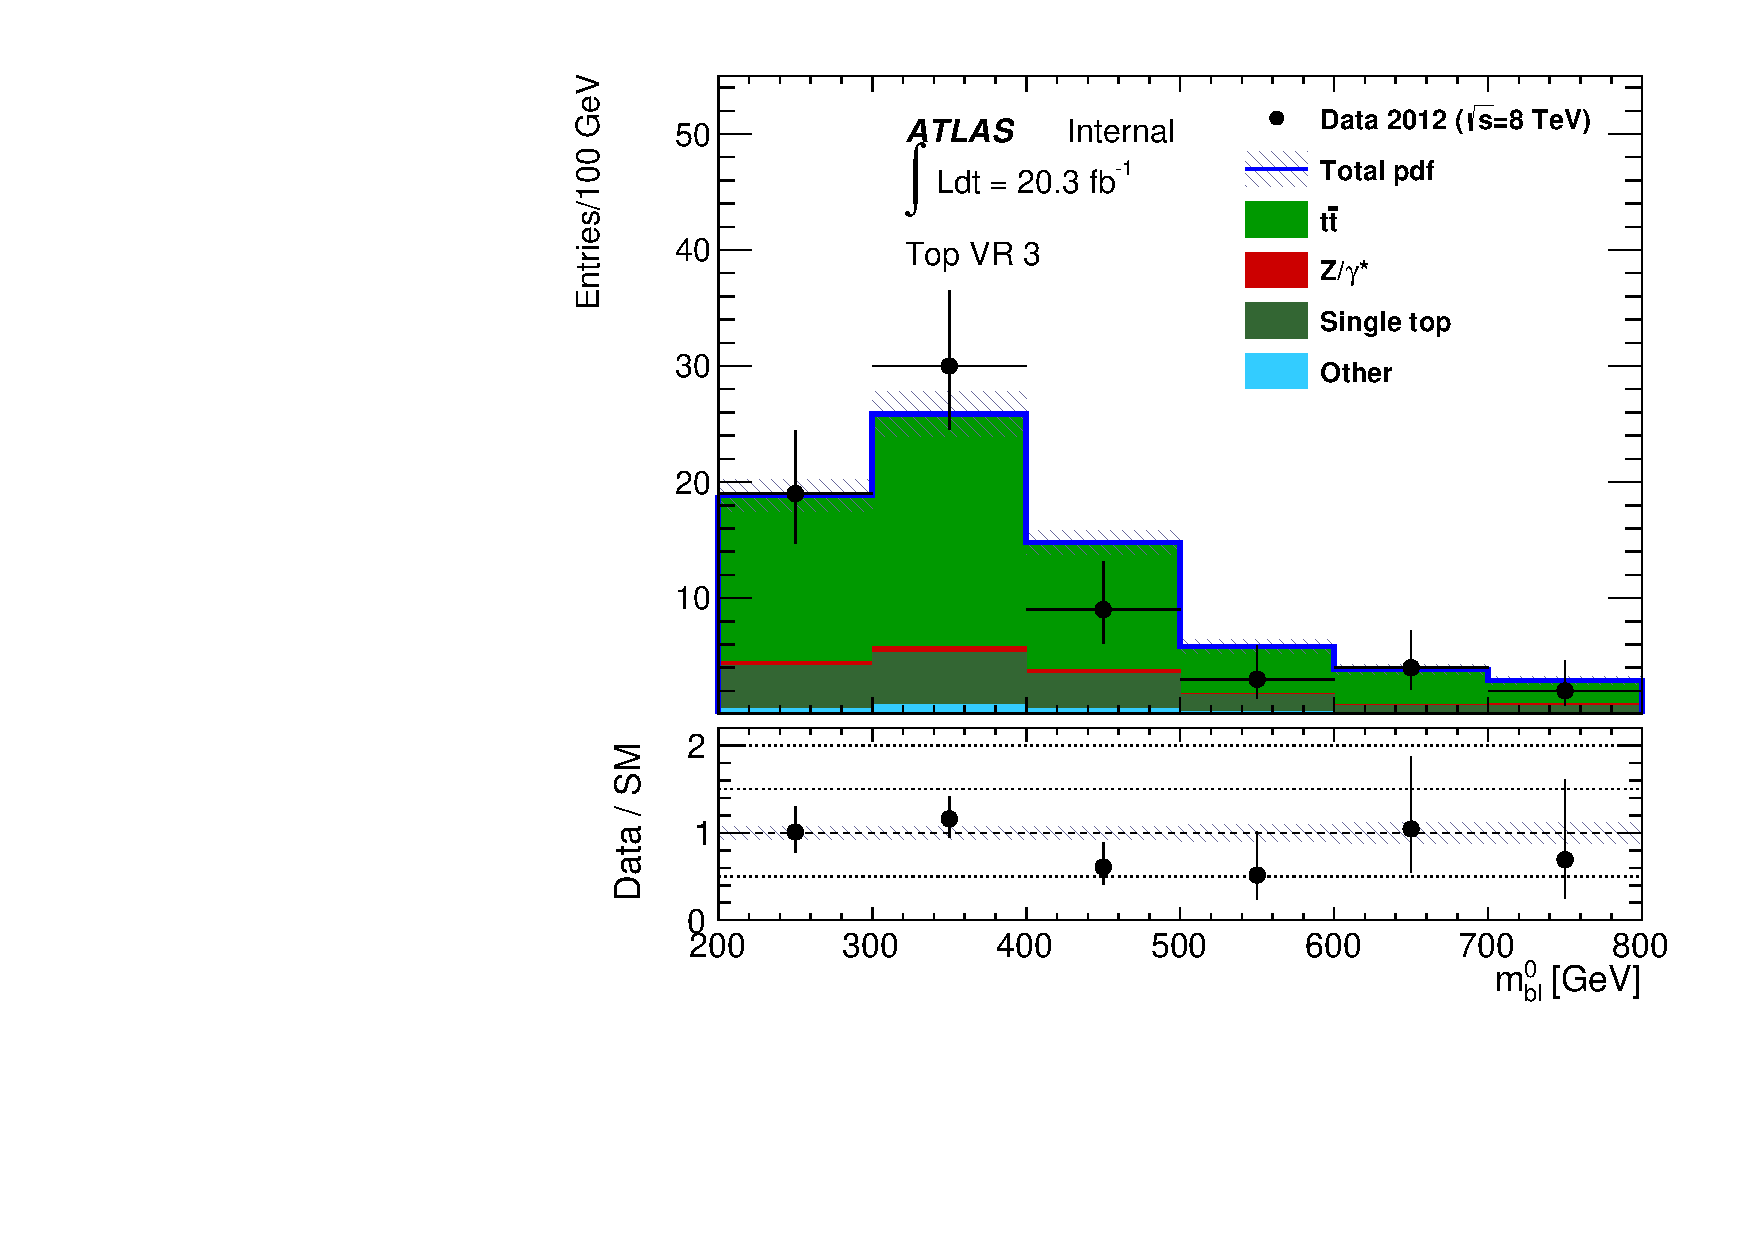
\includegraphics[width=\textwidth]{figures/vr_top_3_mbl_0.pdf}
%%% %%%     \end{block}
%%% %%%   \end{columns}
%%% %%%   %%
%%% %%%   \begin{itemize}
%%% %%%     \item Reasonable agreement in the top background estimate, even out to
%%% %%%       high \Ht
%%% %%%     \item No need for an additional systematic uncertainty on the
%%% %%%       \TTBAR\ background
%%% %%%   \end{itemize}
%%% %%% \end{frame}
%%% %%% 
%%% %%% 
%%% %%% % ------------------------------------------------------------------------------
%%% %%% \begin{frame}
%%% %%%   \frametitle{Z validation region}
%%% %%%   %%
%%% %%%   \begin{columns}
%%% %%%     \column{0.45\textwidth}
%%% %%%     \begin{block}{\Ht}
%%% %%%       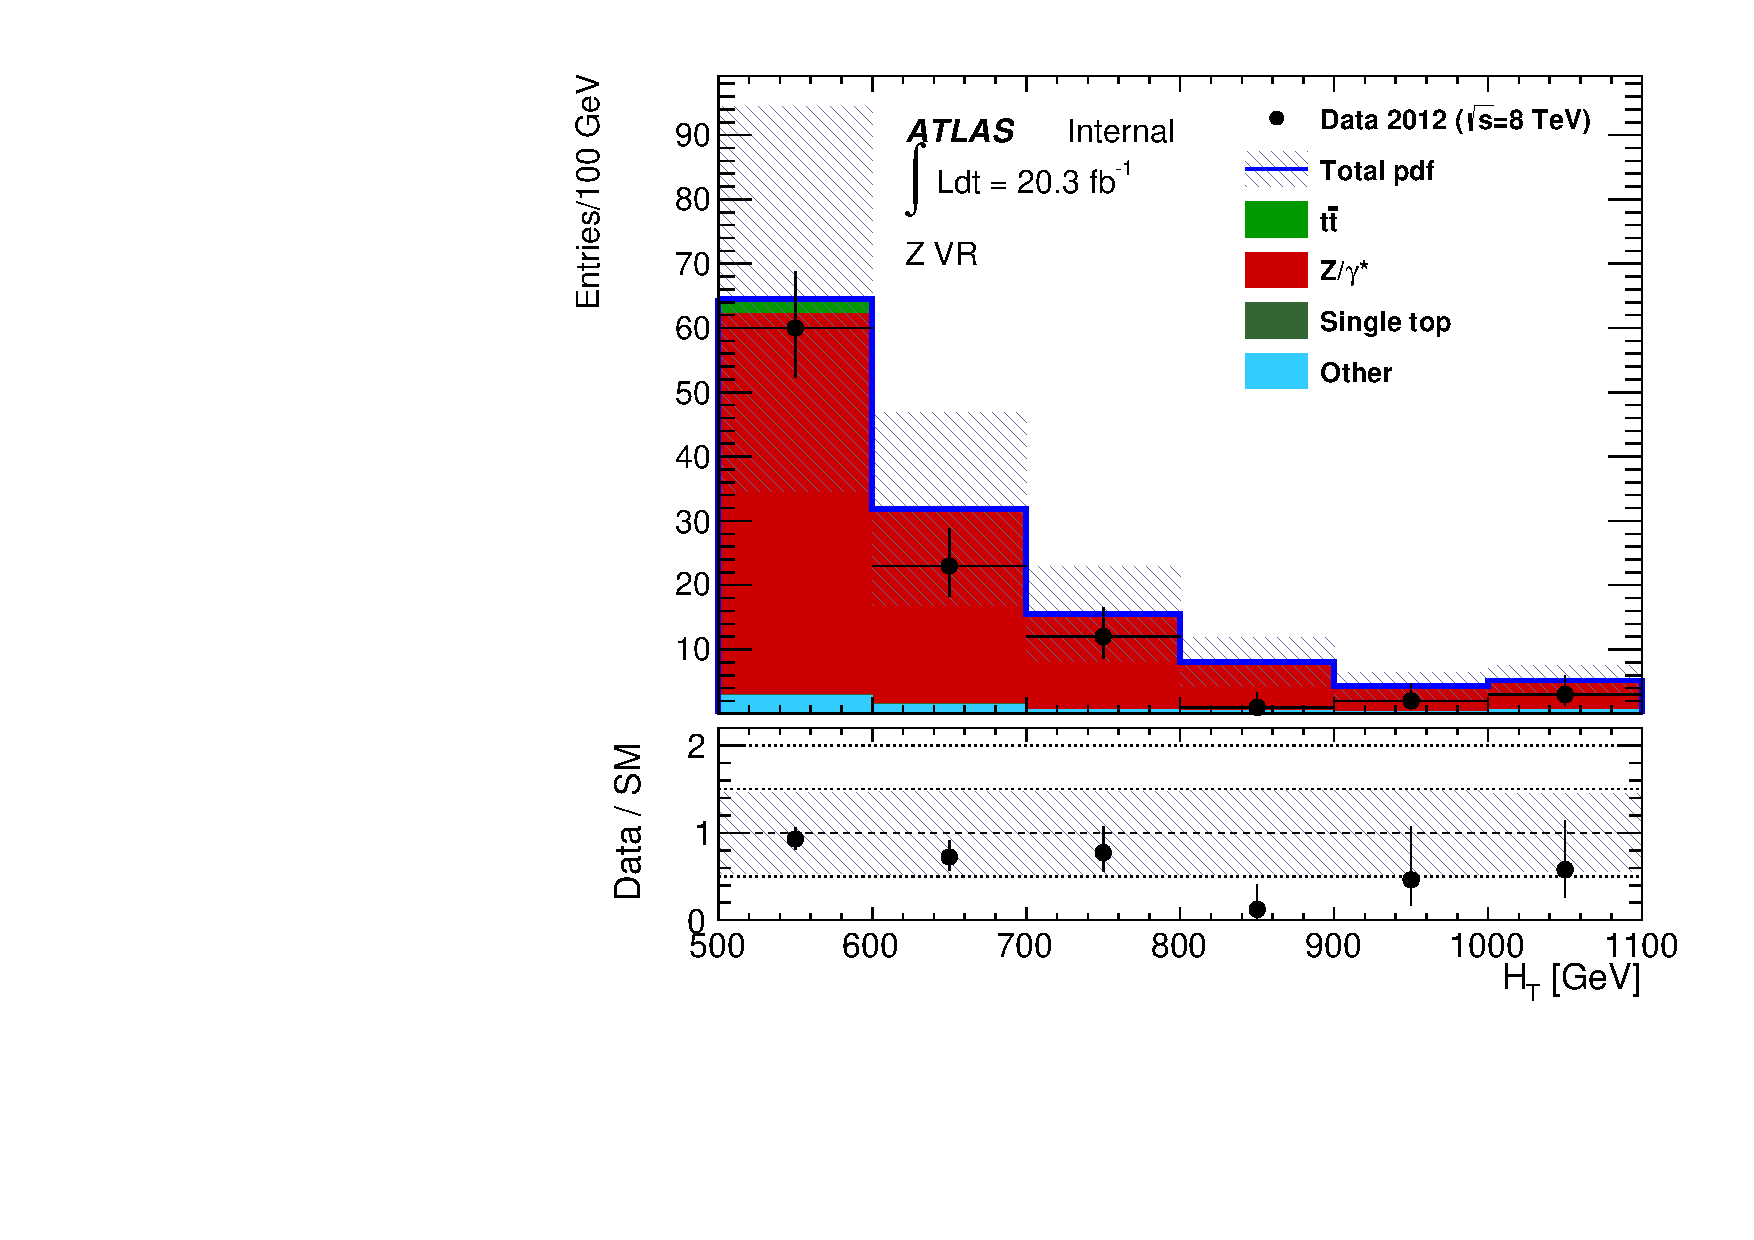
\includegraphics[width=\textwidth]{figures/vr_Z_ht_signal.pdf}
%%% %%%     \end{block}
%%% %%%     \column{0.45\textwidth}
%%% %%%     \begin{block}{\Mbl}
%%% %%%       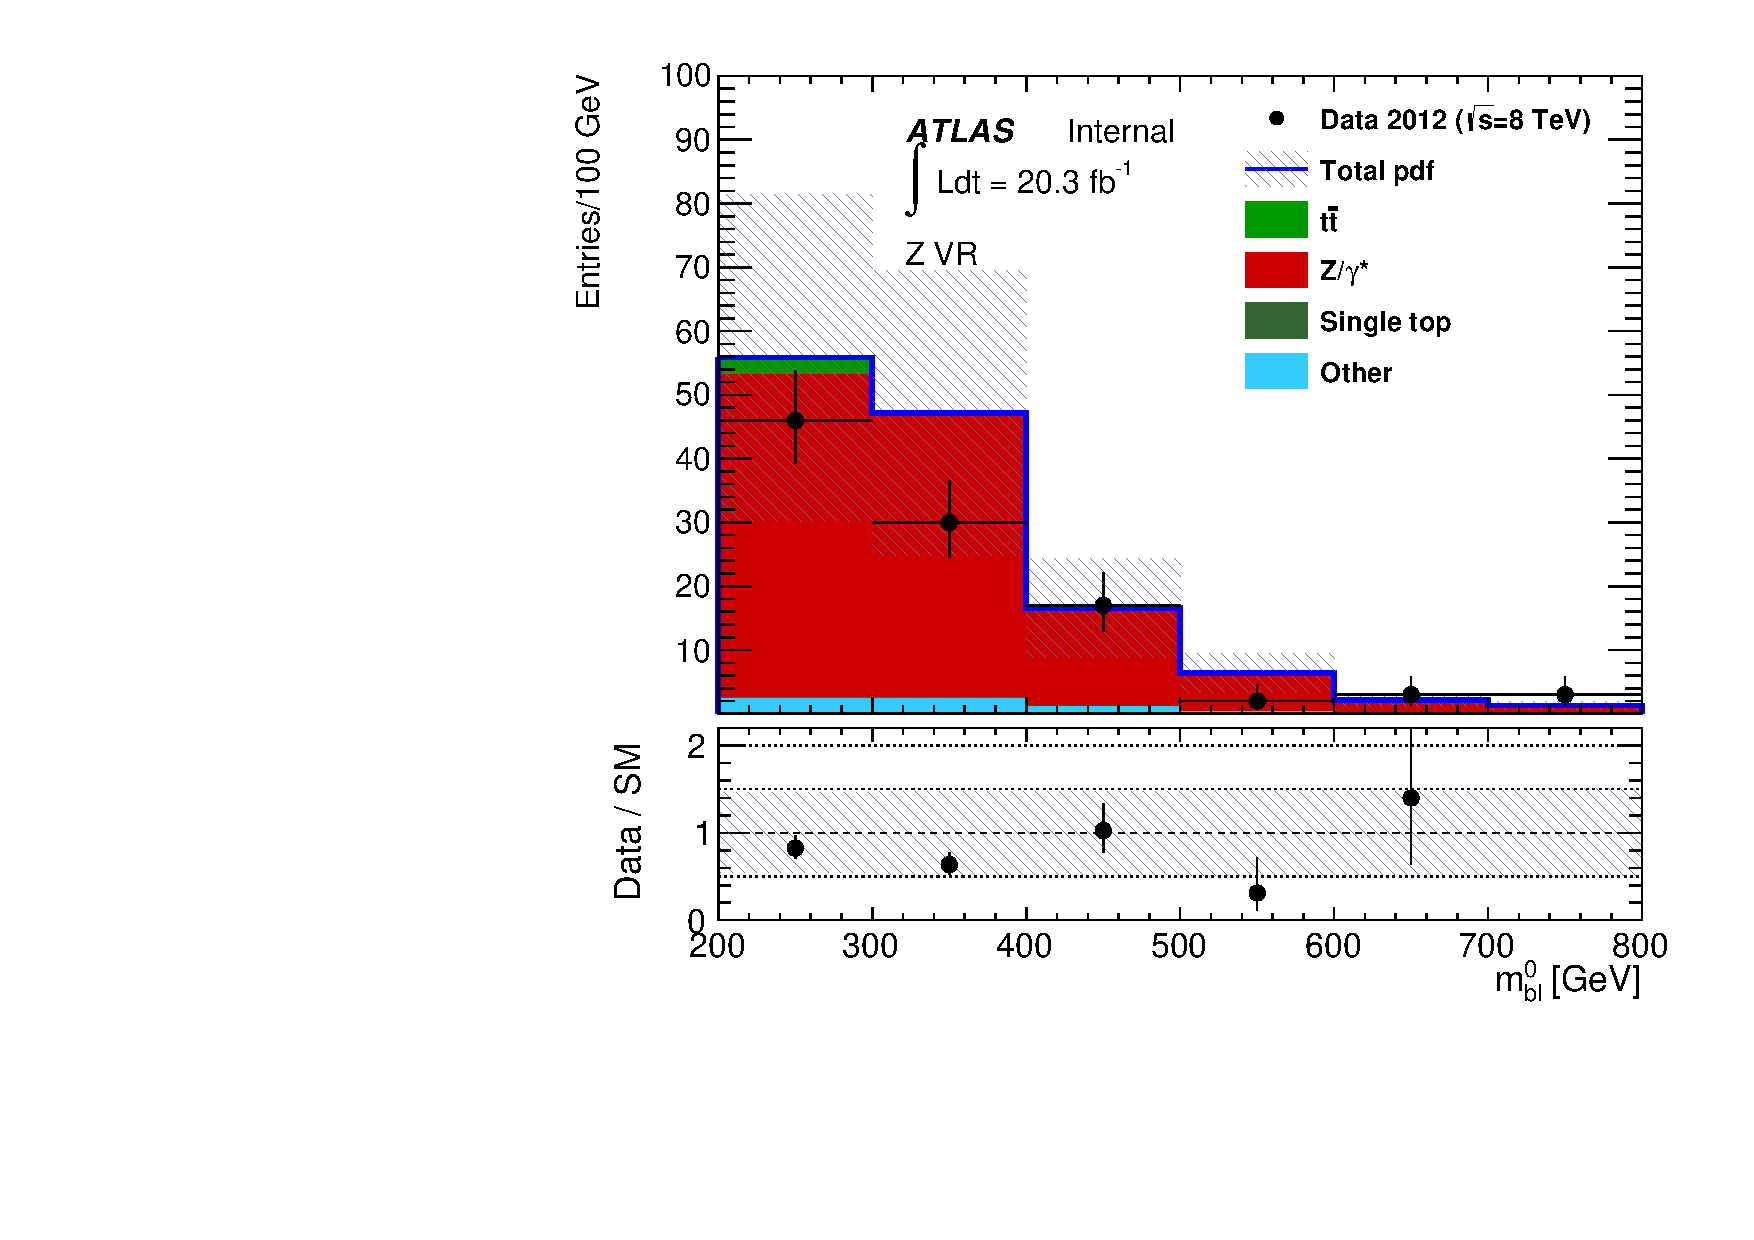
\includegraphics[width=\textwidth]{figures/vr_Z_mbl_0.pdf}
%%% %%%     \end{block}
%%% %%%   \end{columns}
%%% %%%   %%
%%% %%%   \begin{itemize}
%%% %%%     \item \ZGAMMA\ background is overpredicted at high \Ht
%%% %%%     \item For this reason, an additional 50\% systematic uncertainty was taken
%%% %%%       on the \ZGAMMA\ background in regions with high \Ht
%%% %%%   \end{itemize}
%%% %%% \end{frame}
%%% %%% 
%%% %%% 
%%% %%% % ------------------------------------------------------------------------------
%%% %%% \begin{frame}
%%% %%%   \frametitle{Results - SR 400}
%%% %%%   %%
%%% %%%   \begin{center}
%%% %%%     \resizebox{\textwidth}{!}{
%%% %%%       \begin{tabular}{lrrrr}
%%% %%%       \toprule
%%% %%%                                    & SR~400                & SR~400 $ee$           & SR~400 $\mu\mu$       & SR~400 $e\mu$  \\
%%% %%%       \midrule
%%% %%%       Observed                     & $2$                   & $0$                   & $2$                   & $0$                \\
%%% %%%       \midrule
%%% %%%       Fitted bkg                   & $1.39 \pm 0.35$       & $0.36 \pm 0.15$       & $0.57 \pm 0.20$       & $0.45 \pm 0.11$    \\
%%% %%%       \midrule
%%% %%%       Fitted $t\bar{t}$            & $0.33 \pm 0.09$       & $0.07 \pm 0.08$       & $0.07 \pm 0.02$       & $0.19 \pm 0.05$    \\
%%% %%%       Fitted $Z/\gamma^{*}$+jets   & $0.54 \pm 0.28$       & $0.20 \pm 0.10$       & $0.35 \pm 0.18$       & $0.00 \pm 0.00$    \\
%%% %%%       Fitted Single Top            & $0.44 \pm 0.08$       & $0.10 \pm 0.03$       & $0.11 \pm 0.03$       & $0.23 \pm 0.05$    \\
%%% %%%       Fitted Other                 & $0.07 \pm 0.04$       & $0.00 \pm 0.00$       & $0.04 \pm 0.02$       & $0.03 \pm 0.03$    \\
%%% %%%       \midrule
%%% %%%       MC exp. SM                   & $1.2$                 & $0.30$                & $0.46$                & $0.43$             \\
%%% %%%       \midrule
%%% %%%       MC exp. $t\bar{t}$           & $0.30$                & $0.06$                & $0.06$                & $0.17$             \\
%%% %%%       MC exp. $Z/\gamma^{*}$+jets  & $0.38$                & $0.14$                & $0.24$                & $0.00$             \\
%%% %%%       MC exp. Single Top           & $0.44$                & $0.10$                & $0.11$                & $0.23$             \\
%%% %%%       MC exp. Other                & $0.07$                & $0.00$                & $0.04$                & $0.03$             \\
%%% %%%       \midrule
%%% %%%       $\sigma_\mathrm{vis}$~[fb]   & 0.23                  & 0.11                  & 0.26                  & 0.11                  \\
%%% %%%       Observed $N_\mathrm{non-SM}$ & 4.8                   & 2.2                   & 5.4                   & 2.3                   \\
%%% %%%       Expected $N_\mathrm{non-SM}$ & ${4.0}^{+2.2}_{-1.2}$ & ${3.2}^{+1.8}_{-3.2}$ & ${3.6}^{+1.9}_{-1.5}$ & ${3.3}^{+1.8}_{-3.1}$ \\
%%% %%%       \bottomrule
%%% %%%       \end{tabular}
%%% %%%     }
%%% %%%   \end{center}
%%% %%% \end{frame}
%%% %%% 
%%% %%% 
%%% %%% % ------------------------------------------------------------------------------
%%% %%% \begin{frame}
%%% %%%   \frametitle{Results - SR 600}
%%% %%%   %%
%%% %%%   \begin{center}
%%% %%%     \resizebox{\textwidth}{!}{
%%% %%%       \begin{tabular}{lrrrr}
%%% %%%       \toprule
%%% %%%                                    & SR~600                & SR~600 $ee$           & SR~600 $\mu\mu$       & SR~600 $e\mu$   \\
%%% %%%       \midrule
%%% %%%       Observed                     & $1$                   & $0$                   & $1$                   & $0$              \\
%%% %%%       \midrule
%%% %%%       Fitted bkg                   & $0.55 \pm 0.15$       & $0.15 \pm 0.06$       & $0.24 \pm 0.10$       & $0.16 \pm 0.06$  \\
%%% %%%       \midrule
%%% %%%       Fitted $t\bar{t}$            & $0.10 \pm 0.02$       & $0.03 \pm 0.01$       & $0.00 \pm 0.00$       & $0.07 \pm 0.03$  \\
%%% %%%       Fitted $Z/\gamma^{*}$+jets   & $0.23 \pm 0.12$       & $0.08 \pm 0.05$       & $0.15 \pm 0.08$       & $0.00 \pm 0.00$  \\
%%% %%%       Fitted Single Top            & $0.18 \pm 0.04$       & $0.03 \pm 0.01$       & $0.05 \pm 0.02$       & $0.09 \pm 0.03$  \\
%%% %%%       Fitted Other                 & $0.04 \pm 0.01$       & $0.00 \pm 0.00$       & $0.04 \pm 0.02$       & $0.00 \pm 0.00$  \\
%%% %%%       \midrule
%%% %%%       MC exp. SM                   & $0.47$                & $0.12$                & $0.20$                & $0.16$           \\
%%% %%%       \midrule
%%% %%%       MC exp. $t\bar{t}$           & $0.09$                & $0.03$                & $0.00$                & $0.06$           \\
%%% %%%       MC exp. $Z/\gamma^{*}$+jets  & $0.16$                & $0.06$                & $0.10$                & $0.00$           \\
%%% %%%       MC exp. Single Top           & $0.18$                & $0.03$                & $0.05$                & $0.09$           \\
%%% %%%       MC exp. Other                & $0.04$                & $0.00$                & $0.04$                & $0.00$           \\
%%% %%%       \midrule
%%% %%%       $\sigma_\mathrm{vis}$~[fb]   & 0.19                  & 0.10                  & 0.20                  & 0.10 \\
%%% %%%       Observed $N_\mathrm{non-SM}$ & 3.9                   & 2.1                   & 4.0                   & 2.1 \\
%%% %%%       Expected $N_\mathrm{non-SM}$ & ${3.5}^{+1.9}_{-1.4}$ & ${2.6}^{+1.6}_{-0.6}$ & ${3.0}^{+1.7}_{-1.0}$ & ${2.7}^{+1.6}_{-0.7}$ \\
%%% %%%       \bottomrule
%%% %%%       \end{tabular}
%%% %%%     }
%%% %%%   \end{center}
%%% %%% \end{frame}
%%% %%% 
%%% %%% 
%%% %%% % ------------------------------------------------------------------------------
%%% %%% \begin{frame}
%%% %%%   \frametitle{Results - Event kinematics}
%%% %%%   \begin{center}
%%% %%%     \resizebox{0.5\textwidth}{!}{
%%% %%%       \begin{tabular}{lcc}
%%% %%%         \toprule
%%% %%%         Run number                   & 214216    & 210302     \\
%%% %%%         Event number                 & 121272046 & 2292645861 \\
%%% %%%         \midrule
%%% %%%         $\Mbl^0$ [GeV]               & 558   & 686   \\
%%% %%%         %                                              
%%% %%%         $\ell_0$ flavor              & $\mu$ & $\mu$ \\
%%% %%%         $\ell_0$ charge              & -     & -     \\
%%% %%%         %                                              
%%% %%%         $\ell_0\ p_\mathrm{T}$ [GeV] & 375   & 272   \\
%%% %%%         $b_0\ p_\mathrm{T}$    [GeV] & 330   & 460   \\
%%% %%%         %                                              
%%% %%%         $\ell_0\ \eta$               & -0.11 & 1.22  \\
%%% %%%         $b_0\ \eta$                  & 0.56  & 0.95  \\
%%% %%%         %                                              
%%% %%%         $\ell_0\ \phi$               & 2.0   & -1.3  \\
%%% %%%         $b_0\ \phi$                  & -2.7  & 2.5   \\
%%% %%%         %                                              
%%% %%%         \midrule                                       
%%% %%%         $\Mbl^1$ [GeV]               & 526   & 528   \\
%%% %%%         %                                              
%%% %%%         $\ell_1$ flavor              & $\mu$ & $\mu$ \\
%%% %%%         $\ell_1$ charge              & +     & +     \\
%%% %%%         %                                              
%%% %%%         $\ell_1\ p_\mathrm{T}$ [GeV] & 88    & 96    \\
%%% %%%         $b_1\ p_\mathrm{T}$    [GeV] & 542   & 374   \\
%%% %%%         %                                              
%%% %%%         $\ell_1\ \eta$               & 0.45  & 1.43  \\
%%% %%%         $b_1\ \eta$                  & -1.1  & -0.26 \\
%%% %%%         %                                              
%%% %%%         $\ell_1\ \phi$               & -2.3  & -0.91 \\
%%% %%%         $b_1\ \phi$                  & -0.21 & 2.3   \\
%%% %%%         %                                              
%%% %%%         \midrule                                       
%%% %%%         \MblAsym                     & 0.03  & 0.13  \\
%%% %%%         \Ht\ [GeV]                   & 1335  & 1203  \\
%%% %%%         \MetSig\ $[GeV^{1/2}]$       & 2.9   & 6.4   \\
%%% %%%         \Met\ [GeV]                  & 107   & 223   \\
%%% %%%         $m_{\ell\ell}$ [GeV]         & 324   & 71    \\
%%% %%%         \bottomrule
%%% %%%       \end{tabular}
%%% %%%     }
%%% %%%   \end{center}
%%% %%% \end{frame}
%%% %%% 
%%% %%% 
%%% %%% % ------------------------------------------------------------------------------
%%% %%% \begin{frame}
%%% %%%   \frametitle{Exclusion limits}
%%% %%%   \begin{center}
%%% %%%     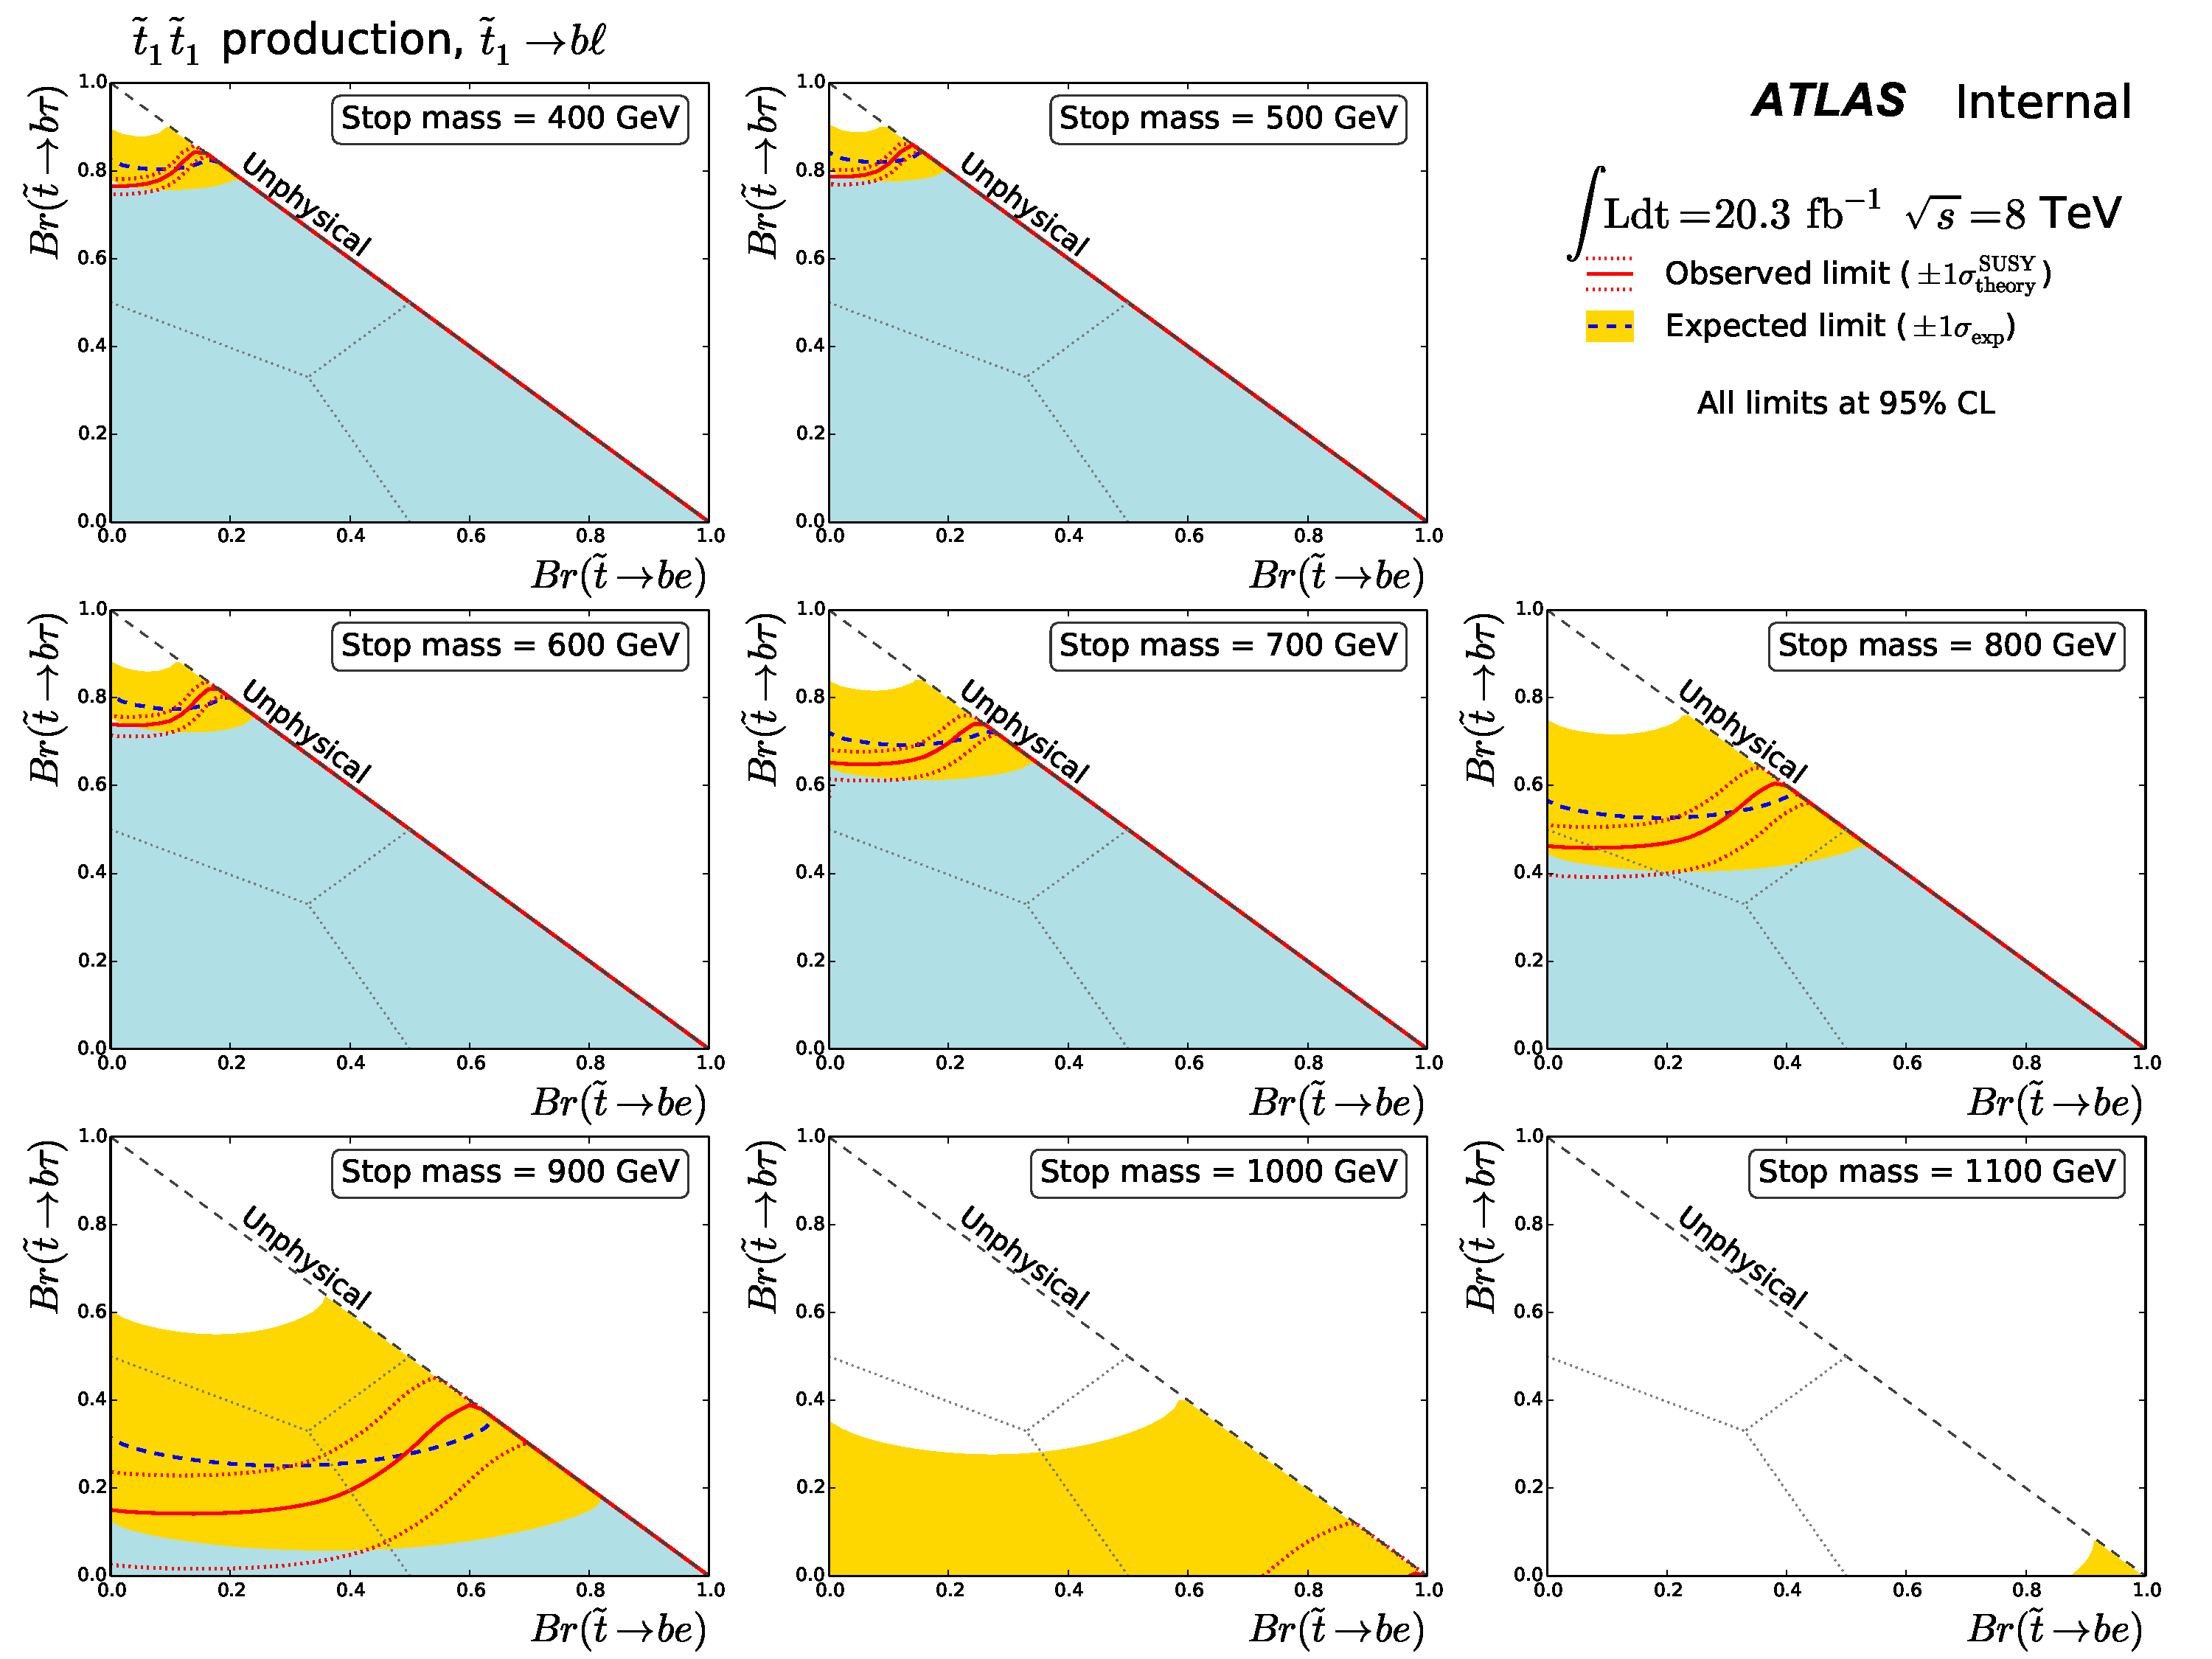
\includegraphics[width=0.9\textwidth]{figures/limit_contours.pdf}
%%% %%%   \end{center}
%%% %%% \end{frame}
%%% %%% 
%%% %%% 
%%% %%% % ------------------------------------------------------------------------------
%%% %%% \begin{frame}
%%% %%%   \frametitle{Exclusion limits}
%%% %%%   \begin{center}
%%% %%%     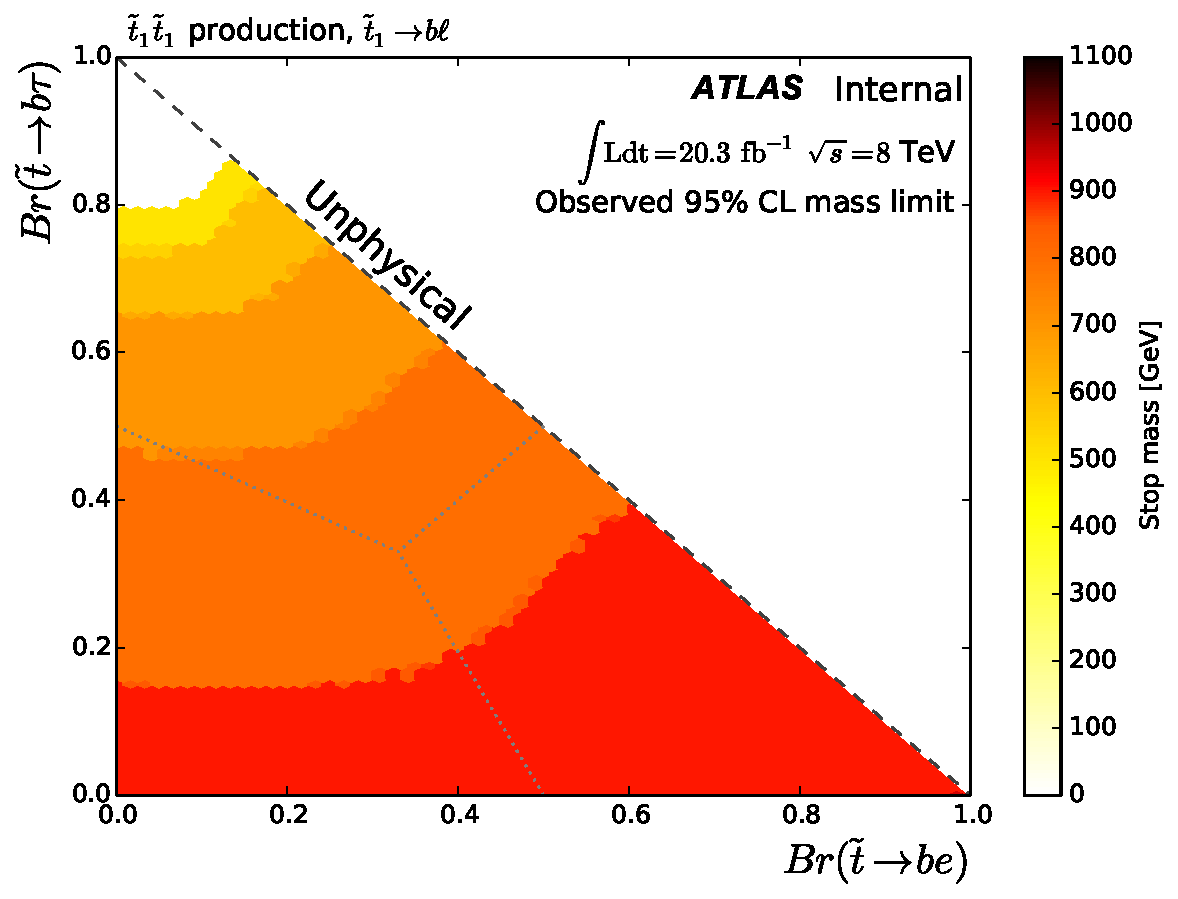
\includegraphics[width=0.9\textwidth]{figures/mass_limit_obs.pdf}
%%% %%%   \end{center}
%%% %%% \end{frame}
%%% %%% 
%%% %%% 
%%% %%% % ------------------------------------------------------------------------------
%%% %%% \begin{frame}
%%% %%%   \frametitle{Conclusions}
%%% %%%   {
%%% %%%     \small
%%% %%%   A search for direct stop production is presented where the stop particles each
%%% %%%   decay via an R-Parity violating coupling to a b quark and an electron or
%%% %%%   muon, leading to final states with two b-tagged jets and two light leptons.
%%% %%%   No significant excess of events above the Standard Model prediction is
%%% %%%   observed, and 95\% confidence limits are set on the mass of the stop.
%%% %%%   A scan of possible stop branching ratios are tested, the mass limit ranges
%%% %%%   between 500 GeV when the stop decays mostly to a b quark and a tau lepton to
%%% %%%   1 TeV when the stop decays mostly to a b quark and an electron.
%%% %%% }
%%% %%% \vspace{1ex}
%%% %%%   \begin{itemize}
%%% %%%     \item First analysis targeting this model!
%%% %%%   \end{itemize}
%%% %%%   \begin{columns}
%%% %%%     \column{0.5\linewidth}
%%% %%%     \begin{center}
%%% %%%       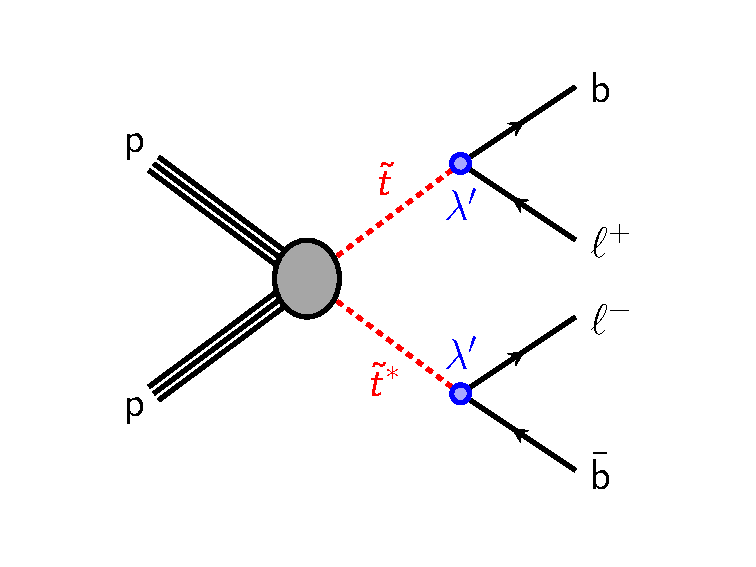
\includegraphics[width=0.9\textwidth]{figures/b_minus_l_stop_stop.pdf}
%%% %%%     \end{center}
%%% %%%     \column{0.5\linewidth}
%%% %%%     \begin{center}
%%% %%%       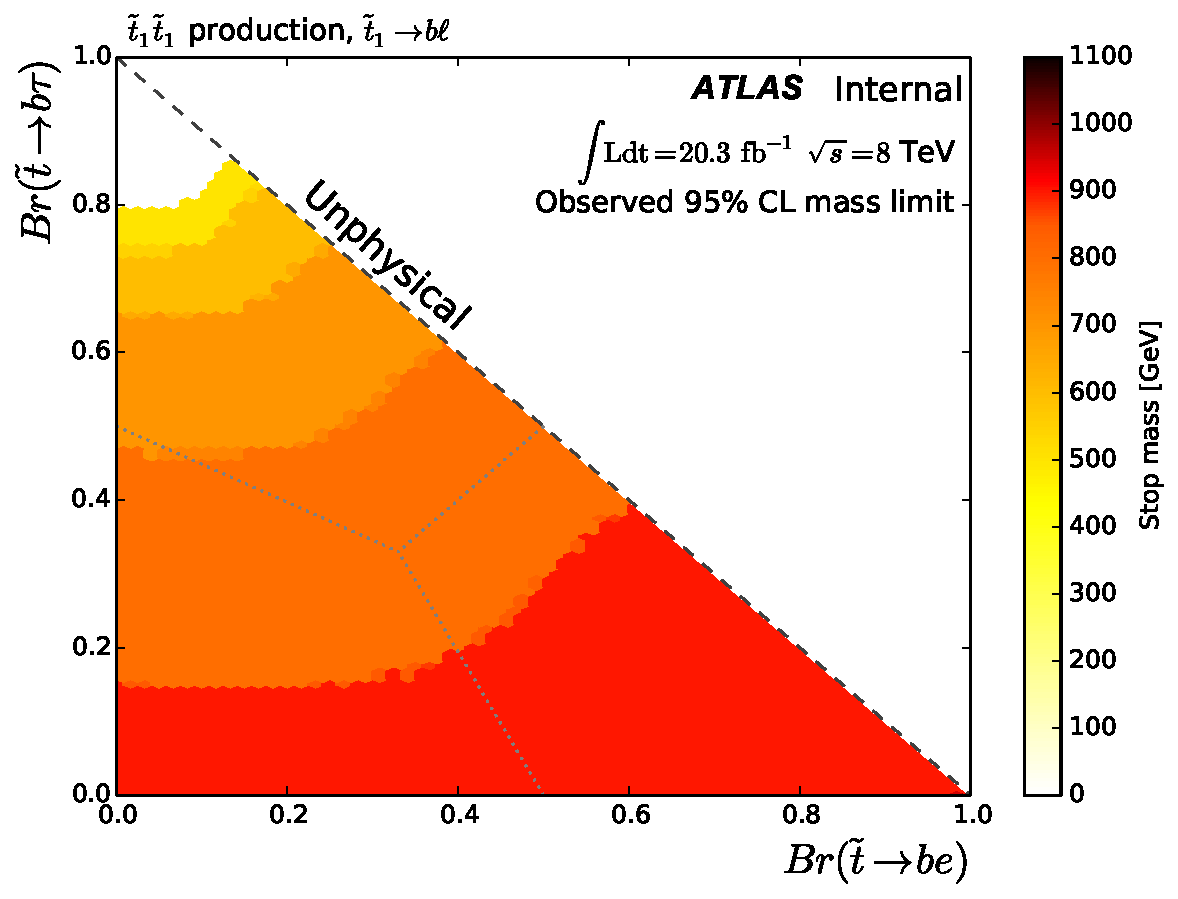
\includegraphics[width=0.9\textwidth]{figures/mass_limit_obs.pdf}
%%% %%%     \end{center}
%%% %%%   \end{columns}
%%% %%% \end{frame}
%%% %%% 
%%% %%% 
%%% %%% %% % ------------------------------------------------------------------------------
%%% %%% %% \begin{frame}
%%% %%% %%   \frametitle{\color{Goldenrod}TODOs!}
%%% %%% %%   %
%%% %%% %%   \begin{itemize}
%%% %%% %%     \item add theorist names
%%% %%% %%   \end{itemize}
%%% %%% %%   %
%%% %%% %% \end{frame}
%%% %%% 
%%% %%% 
%%% %%% % ------------------------------------------------------------------------------
%%% %%% \begin{frame}
%%% %%%   \begin{center}
%%% %%%     {\Huge \color{RoyalBlue} CDS Comments}
%%% %%%   \end{center}
%%% %%% \end{frame}
%%% %%% 
%%% %%% 
%%% %%% % ------------------------------------------------------------------------------
%%% %%% \begin{frame}[t]
%%% %%%   {\color{RoyalBlue}
%%% %%%     From SUSY approval: Define a looser SR for validation — reduce \Mbl\ cut to
%%% %%%     200 GeV — and compare ee/mumu channels, plot lepton pt.
%%% %%%   }
%%% %%%   \begin{itemize}
%%% %%%     \item The following plots are pre-fit, with an ad hoc normalization factor
%%% %%%       applied to the \ZGAMMA\ background
%%% %%%     \item Loosening the \Mbl\ cut to 200 GeV still does not leave us with enough
%%% %%%       statistics to make any statements.
%%% %%%     \item Look instead at the original SR 400 minus the \Ht\ cut
%%% %%%   \end{itemize}
%%% %%%   \begin{columns}
%%% %%%     \column{0.5\textwidth}
%%% %%%     \begin{block}{Flavor channels}
%%% %%%       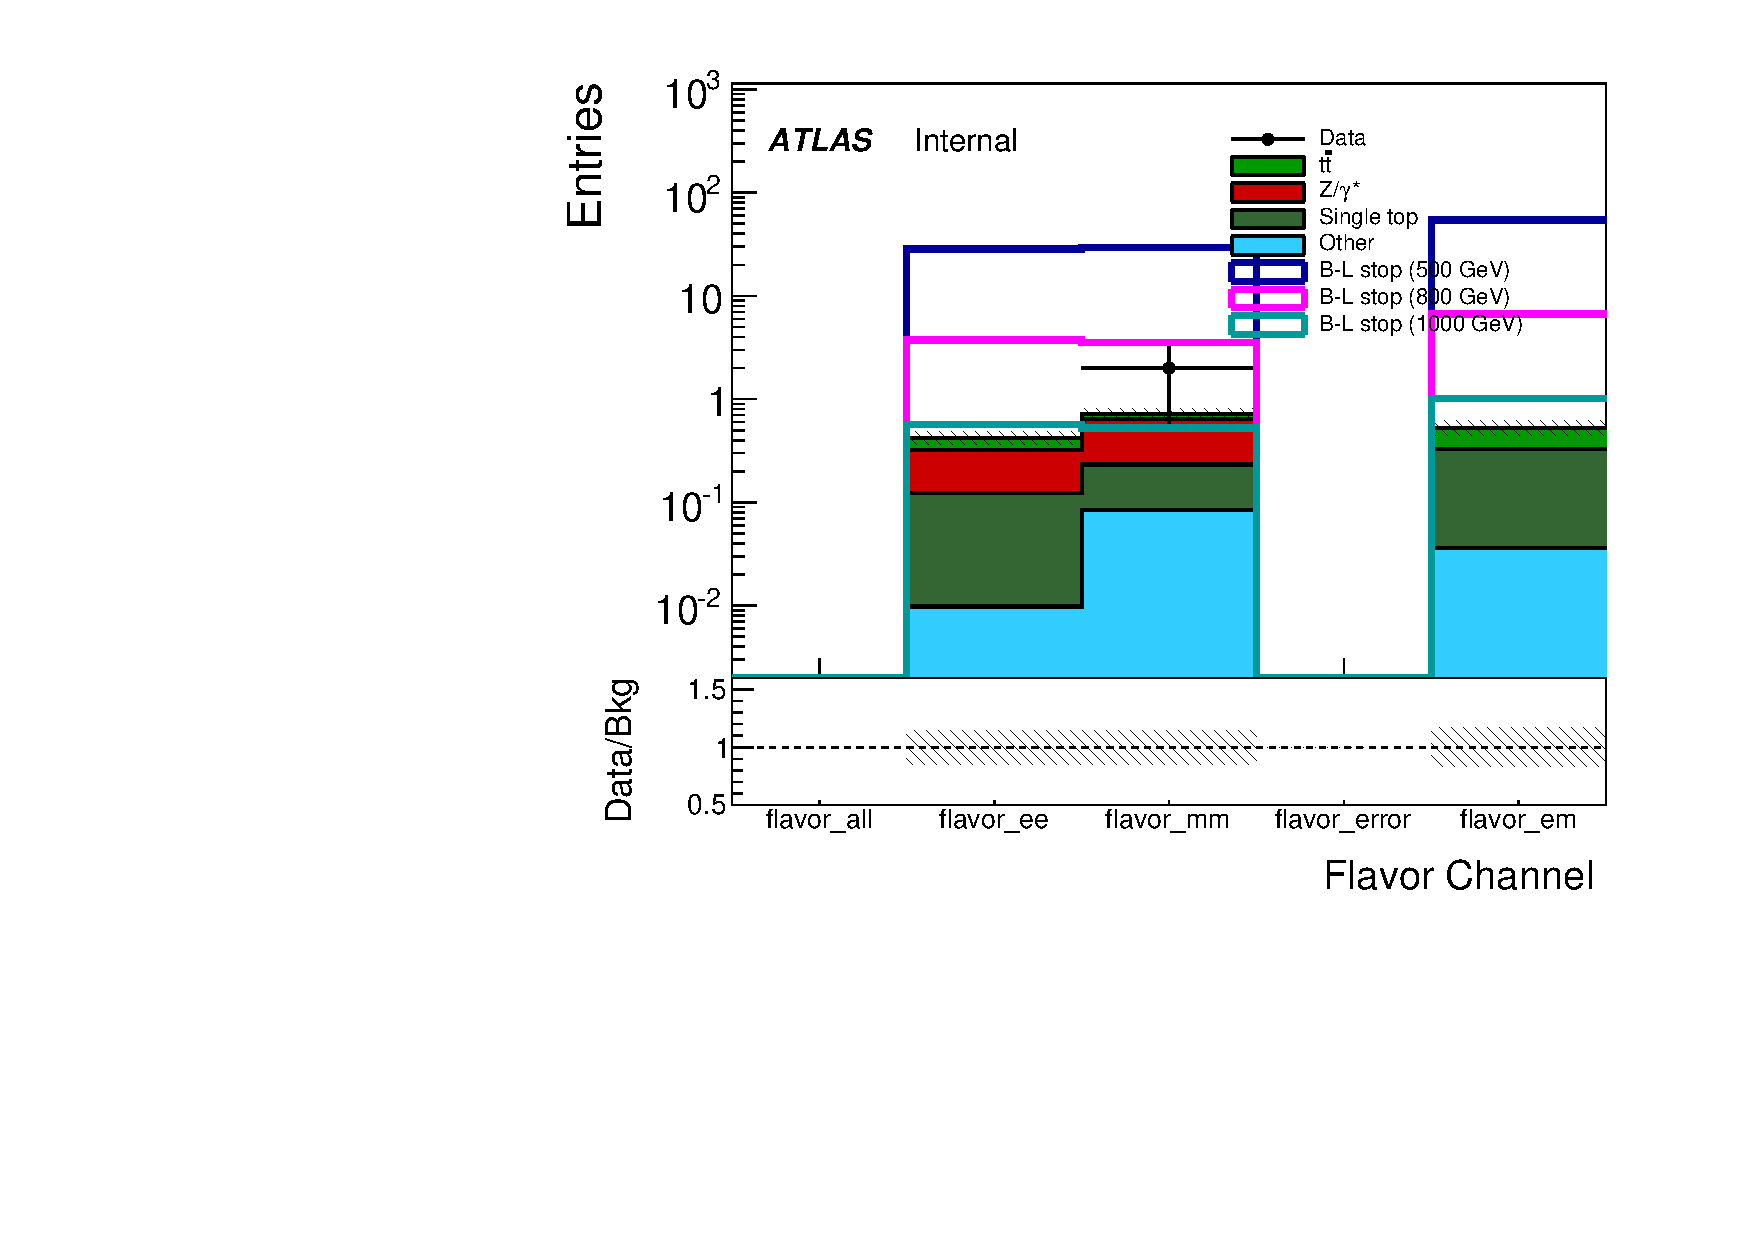
\includegraphics[width=\textwidth]{figures/loose_sr/flavor_all__flavor_channel__BMINUSL_SR_HT_1100_MBL_200__log.pdf}
%%% %%%     \end{block}
%%% %%%     \column{0.5\textwidth}
%%% %%%     \begin{block}{$m_{\ell\ell}$}
%%% %%%       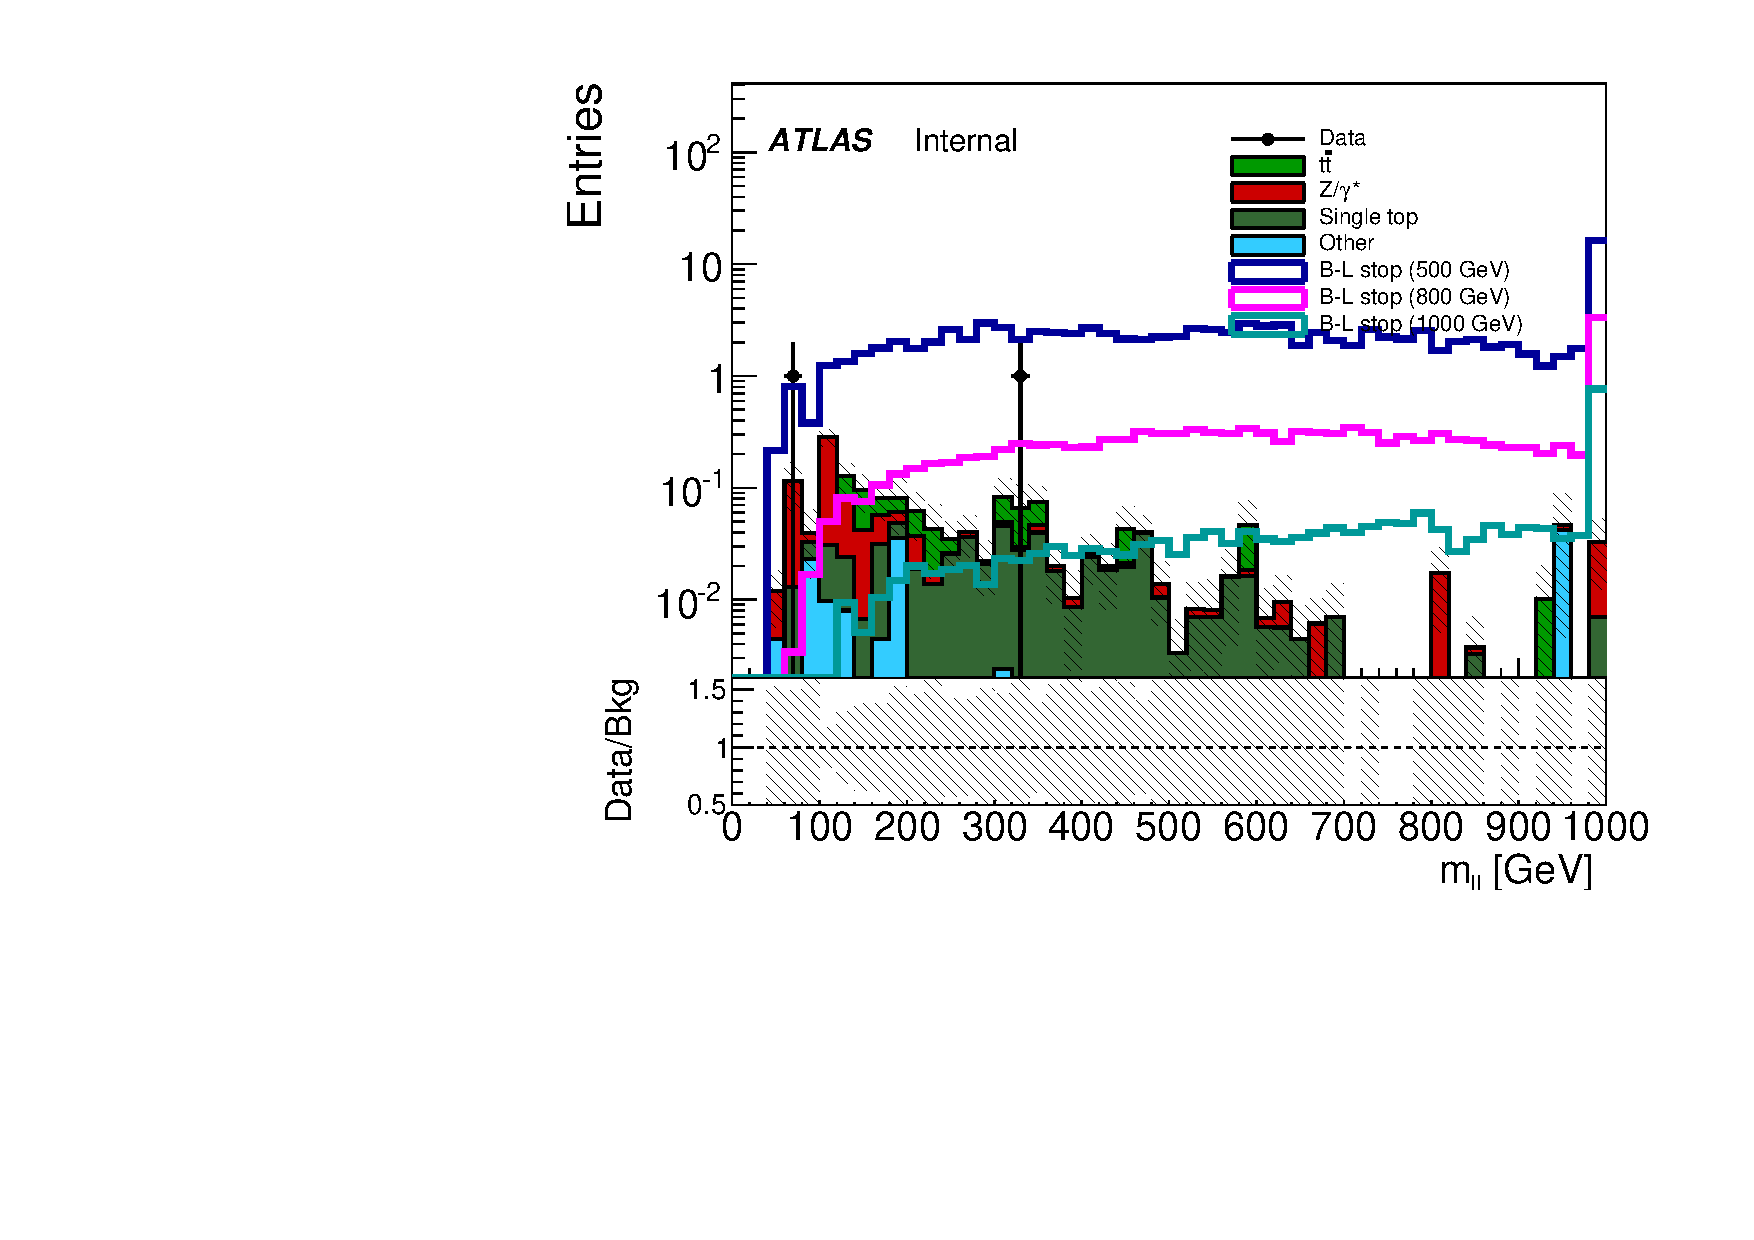
\includegraphics[width=\textwidth]{figures/loose_sr/flavor_all__mll__BMINUSL_SR_HT_1100_MBL_200__log.pdf}
%%% %%%     \end{block}
%%% %%%   \end{columns}
%%% %%% \end{frame}
%%% %%% 
%%% %%% 
%%% %%% % ------------------------------------------------------------------------------
%%% %%% \begin{frame}[t]
%%% %%%   {\color{RoyalBlue}
%%% %%%     From SUSY approval: Define a looser SR for validation — reduce \Mbl\ cut to
%%% %%%     200 GeV — and compare ee/mumu channels, plot lepton pt.
%%% %%%   }
%%% %%%   \begin{itemize}
%%% %%%     \item These plots show the \Ht\ distributions for each flavor channel.
%%% %%%     \item The statistics are still not great, but better than in the previous
%%% %%%       selection
%%% %%%   \end{itemize}
%%% %%%   \begin{columns}
%%% %%%     \column{0.5\textwidth}
%%% %%%     \begin{block}{$ee$ channel}
%%% %%%       \begin{tikzpicture}
%%% %%%         \node[anchor=south west, inner sep=0] (image) at (0,0) {
%%% %%%           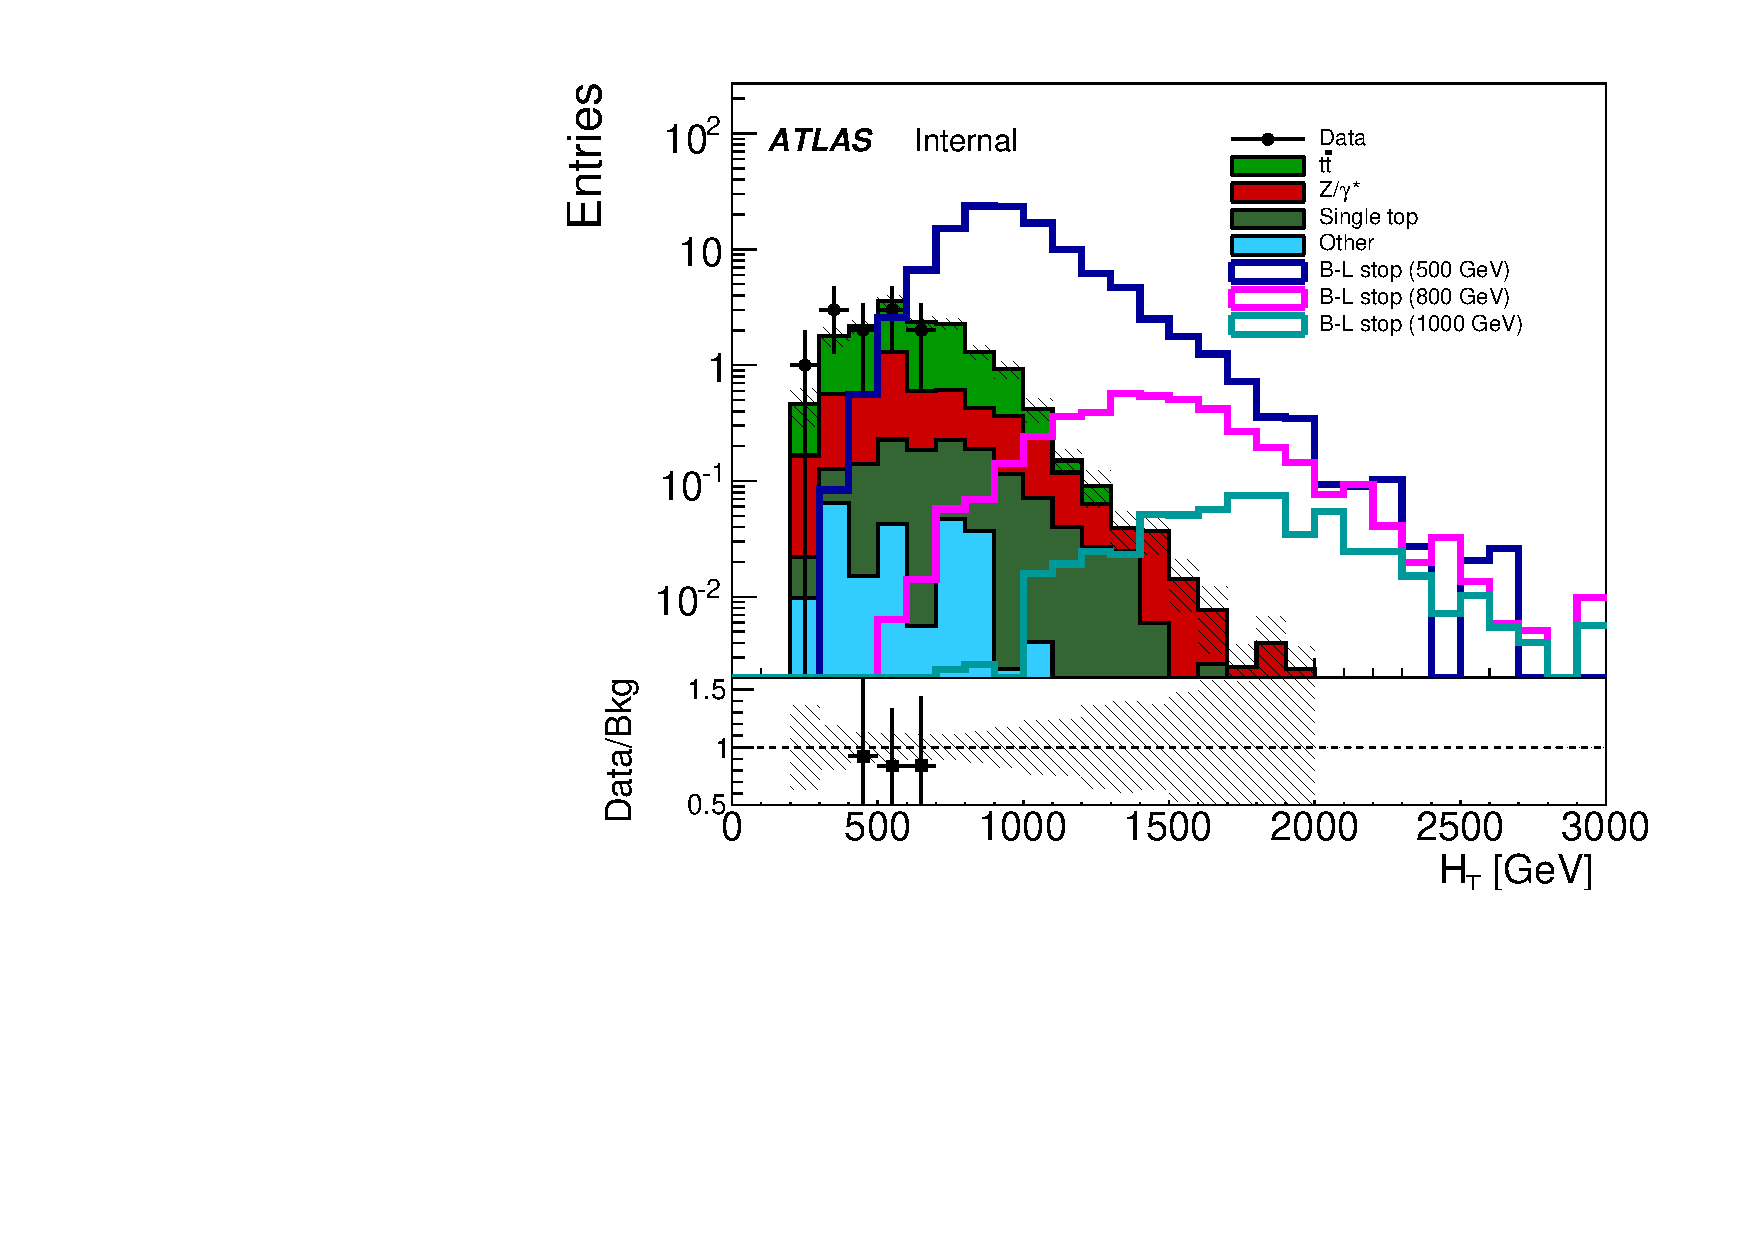
\includegraphics[width=\textwidth]{figures/loose_sr/flavor_ee__ht_signal__BMINUSL_SR_HT_1100_MBL_400_MINUS_HT__log.pdf}
%%% %%%         };
%%% %%%         \begin{scope}[x={(image.south east)}, y={(image.north west)}]
%%% %%%           \draw[color=DarkOrange,   thick] (0.295,0.1) -- (0.295, 0.85);
%%% %%%           \draw[color=MidnightBlue, thick] (0.417,0.1) -- (0.417, 0.85);
%%% %%%           % \MyGrid
%%% %%%         \end{scope}
%%% %%%       \end{tikzpicture}
%%% %%%     \end{block}
%%% %%%     \column{0.5\textwidth}
%%% %%%     \begin{block}{$\mu\mu$ channel}
%%% %%%       \begin{tikzpicture}
%%% %%%         \node[anchor=south west, inner sep=0] (image) at (0,0) {
%%% %%%           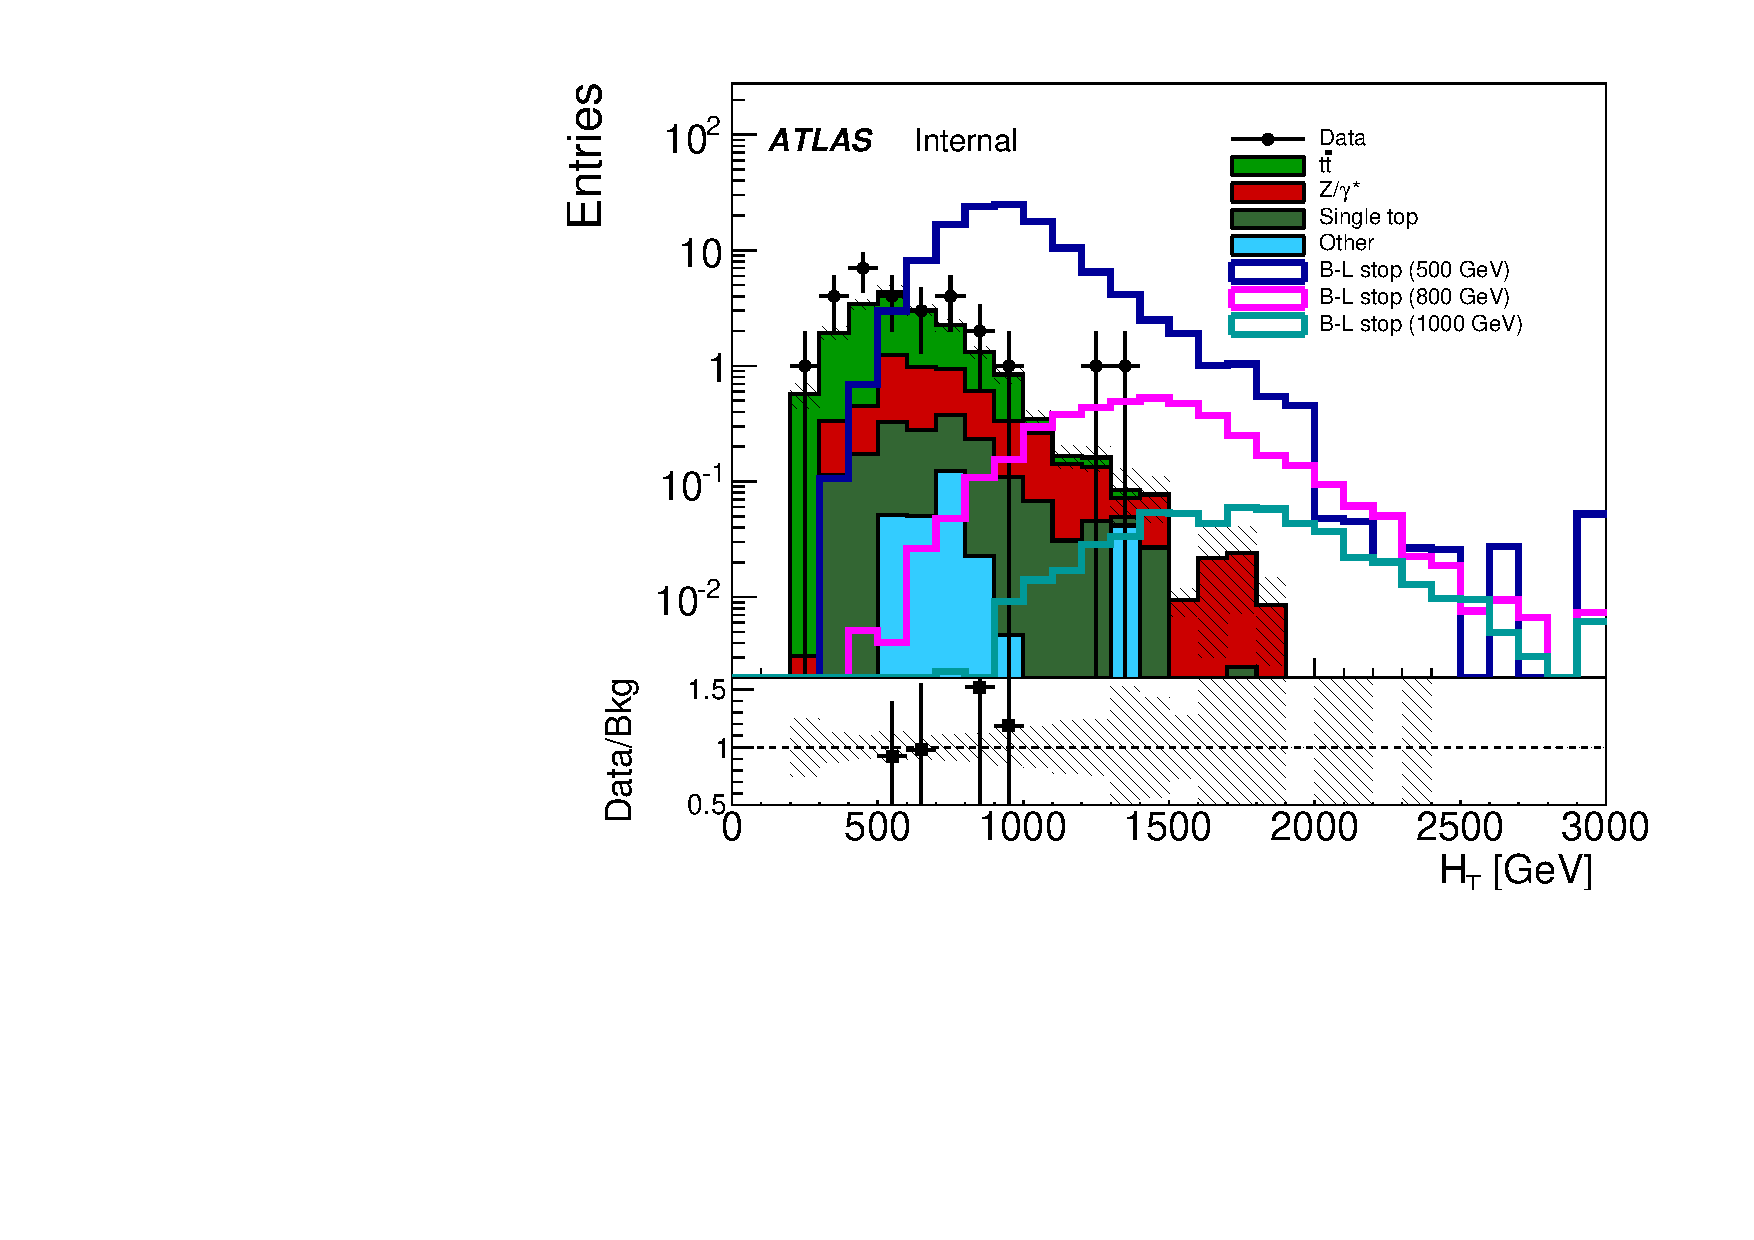
\includegraphics[width=\textwidth]{figures/loose_sr/flavor_mm__ht_signal__BMINUSL_SR_HT_1100_MBL_400_MINUS_HT__log.pdf}
%%% %%%         };
%%% %%%         \begin{scope}[x={(image.south east)}, y={(image.north west)}]
%%% %%%           \draw[color=DarkOrange,   thick] (0.295,0.1) -- (0.295, 0.85);
%%% %%%           \draw[color=MidnightBlue, thick] (0.417,0.1) -- (0.417, 0.85);
%%% %%%           % \MyGrid
%%% %%%         \end{scope}
%%% %%%       \end{tikzpicture}
%%% %%%     \end{block}
%%% %%%   \end{columns}
%%% %%% \end{frame}
%%% %%% 
%%% %%% 
%%% %%% % ------------------------------------------------------------------------------
%%% %%% \begin{frame}[t]
%%% %%%   {\color{RoyalBlue}
%%% %%%     From SUSY approval: Define a looser SR for validation — reduce \Mbl\ cut to
%%% %%%     200 GeV — and compare ee/mumu channels, plot lepton pt.
%%% %%%   }
%%% %%%   \begin{itemize}
%%% %%%     \item These plots show the $p_\mathrm{T}$ distributions for the leading
%%% %%%       lepton in each flavor channel
%%% %%%     \item Despite the low statistics, things don't look very suspicious
%%% %%%   \end{itemize}
%%% %%%   \begin{columns}
%%% %%%     \column{0.5\textwidth}
%%% %%%     \begin{block}{$ee$ channel}
%%% %%%       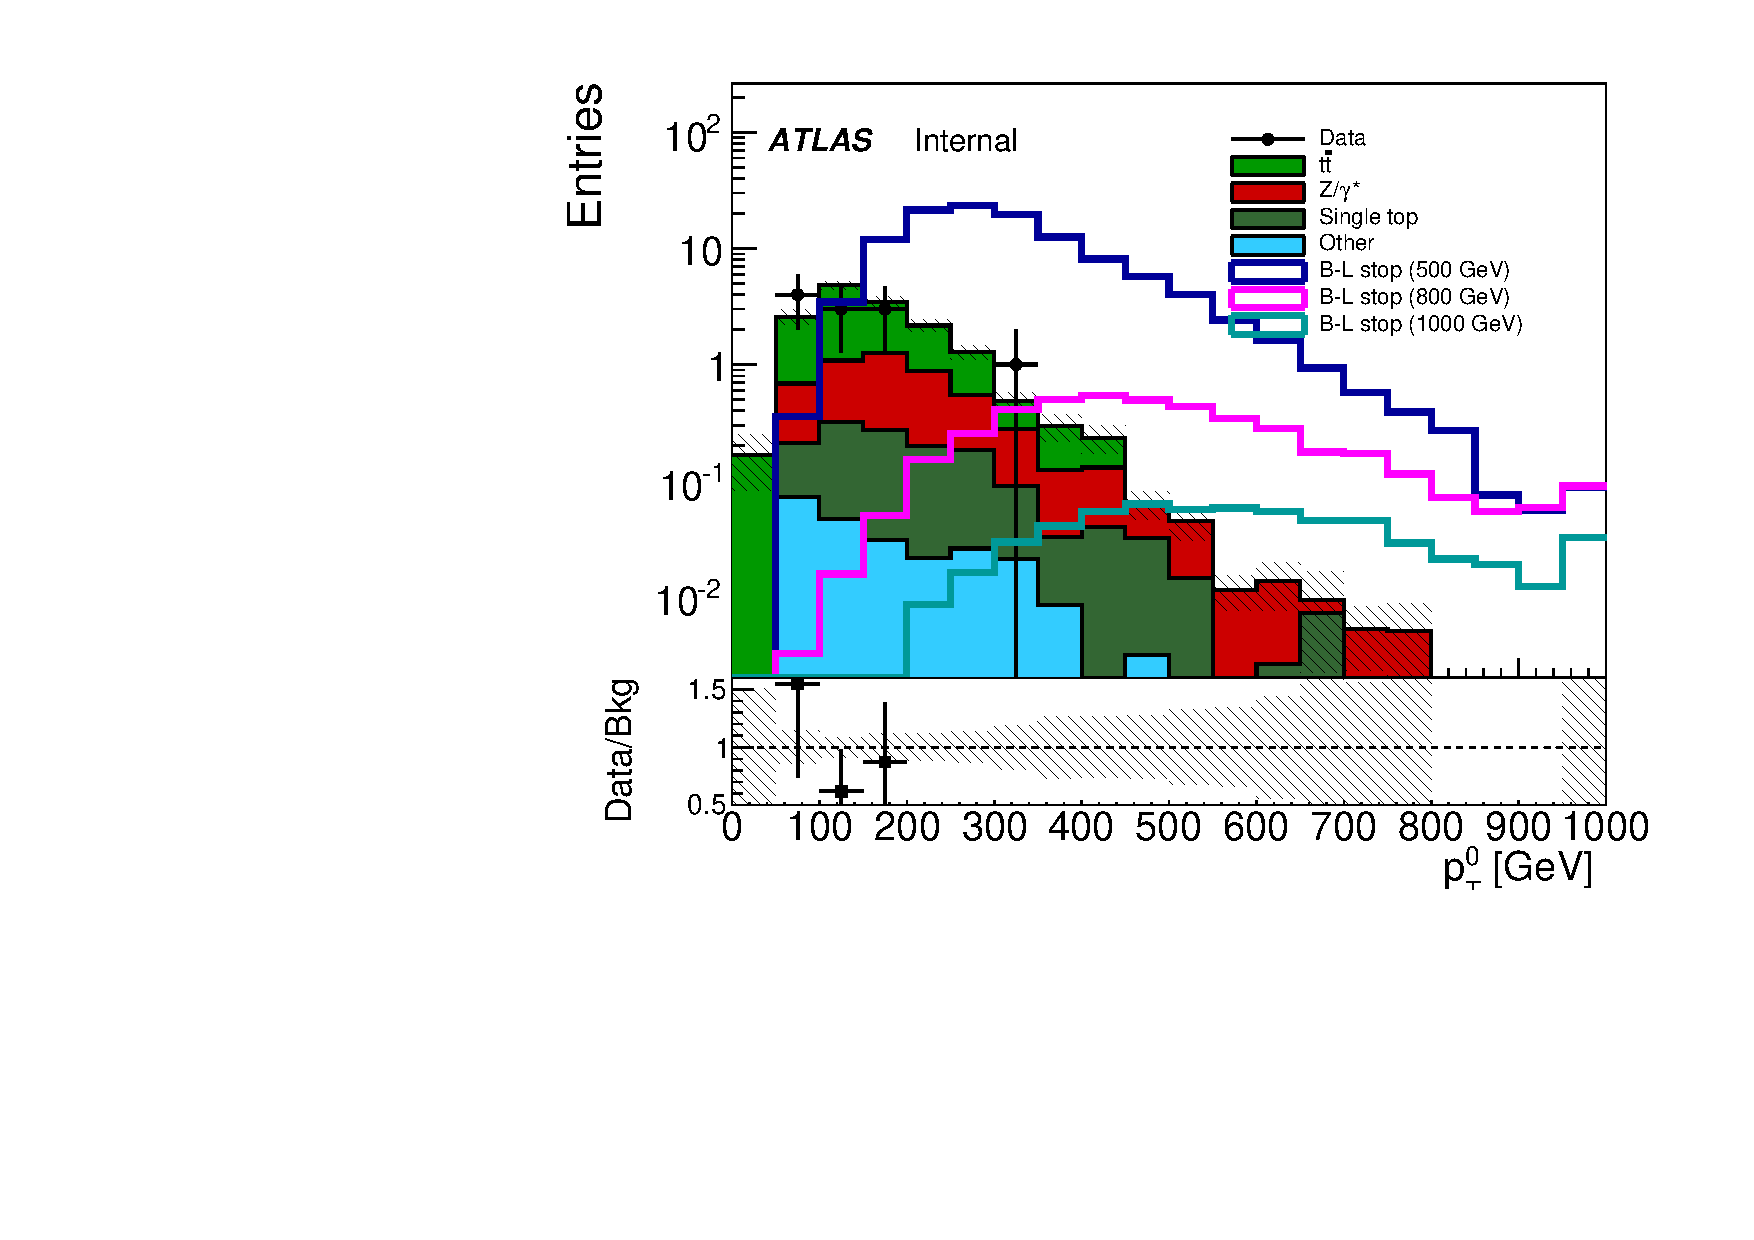
\includegraphics[width=\textwidth]{figures/loose_sr/flavor_ee__lep_pt_0__BMINUSL_SR_HT_1100_MBL_400_MINUS_HT__log.pdf}
%%% %%%     \end{block}
%%% %%%     \column{0.5\textwidth}
%%% %%%     \begin{block}{$\mu\mu$ channel}
%%% %%%       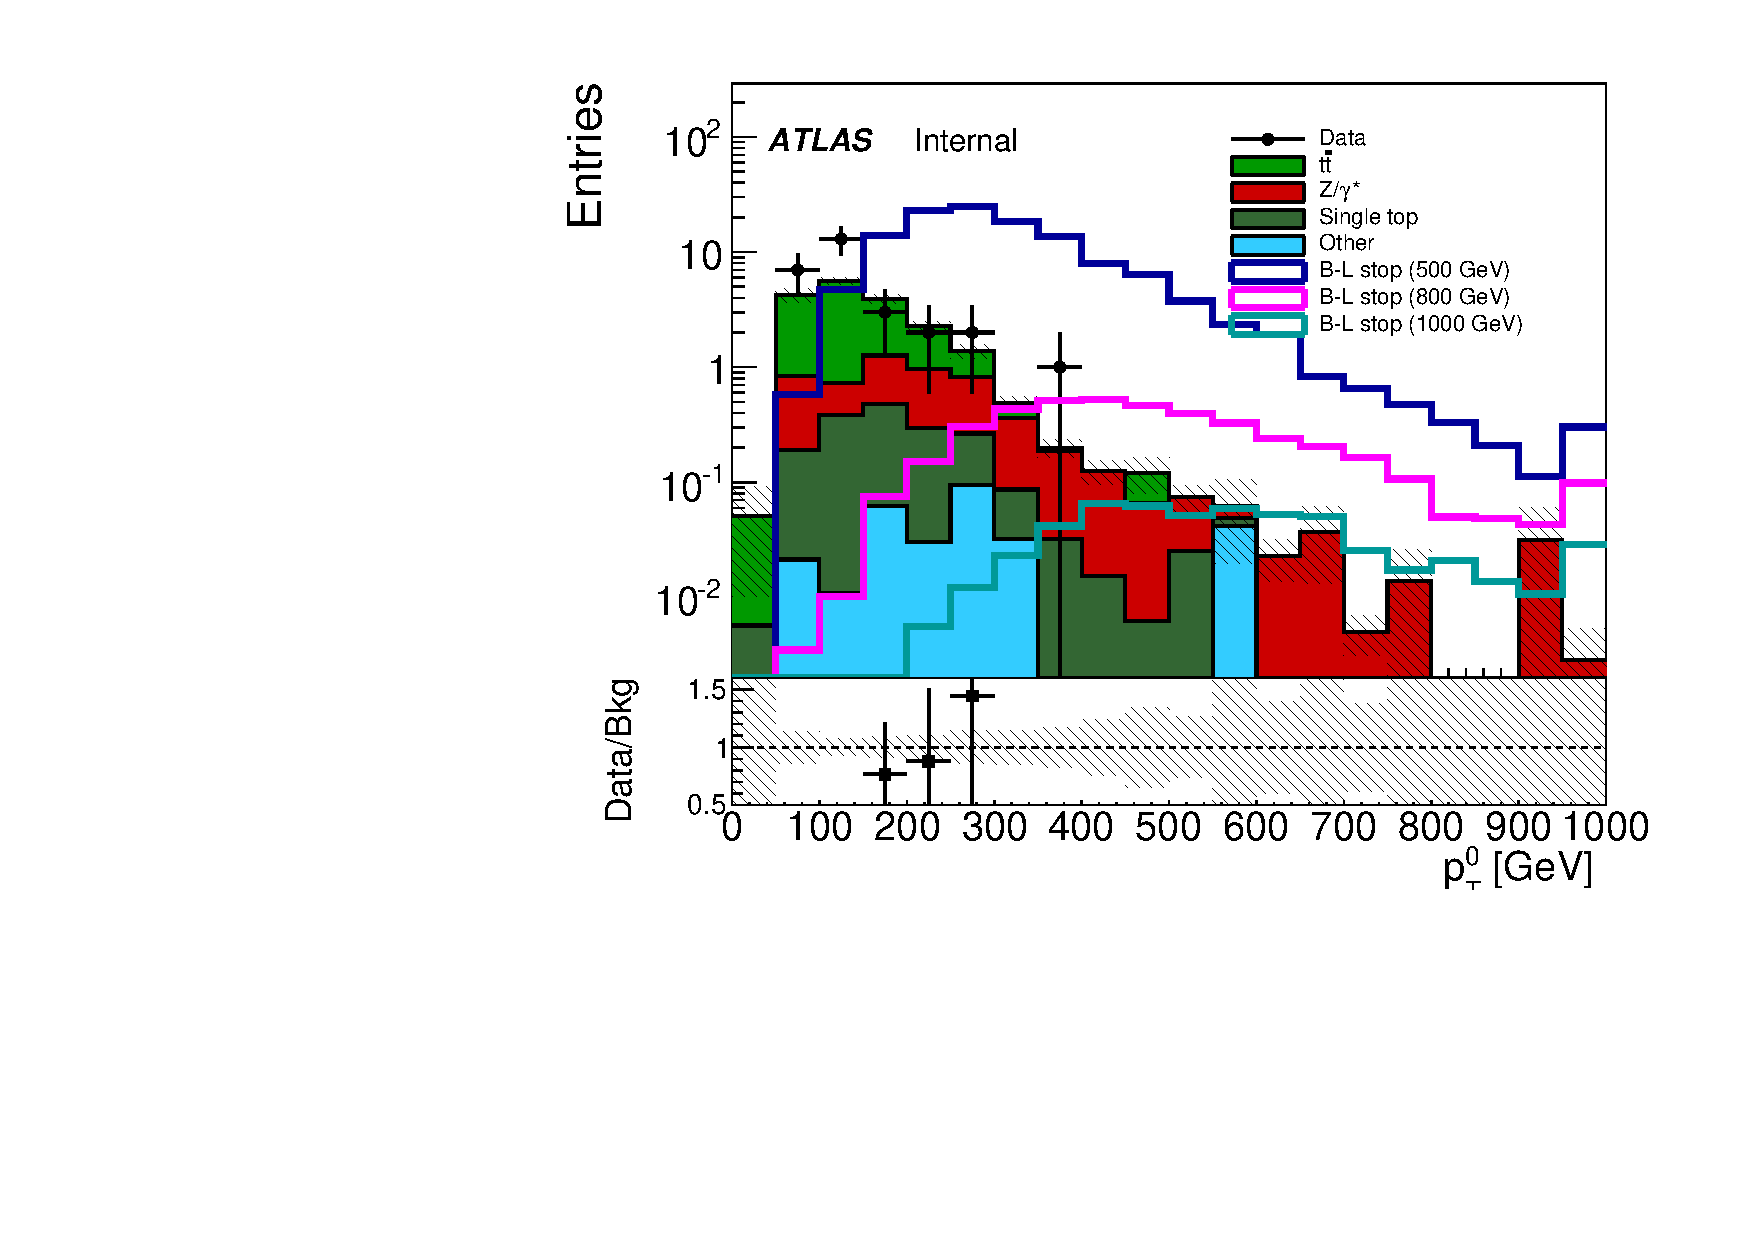
\includegraphics[width=\textwidth]{figures/loose_sr/flavor_mm__lep_pt_0__BMINUSL_SR_HT_1100_MBL_400_MINUS_HT__log.pdf}
%%% %%%     \end{block}
%%% %%%   \end{columns}
%%% %%% \end{frame}
%%% %%% 
%%% %%% 
%%% %%% % ------------------------------------------------------------------------------
%%% %%% \begin{frame}[t]
%%% %%%   {\color{RoyalBlue}
%%% %%%     From SUSY approval: Define a looser SR for validation — reduce \Mbl\ cut to
%%% %%%     200 GeV — and compare ee/mumu channels, plot lepton pt.
%%% %%%   }
%%% %%%   \begin{itemize}
%%% %%%     \item These plots show the $p_\mathrm{T}$ distributions for the sub-leading
%%% %%%       lepton in each flavor channel
%%% %%%     \item Despite the low statistics, things don't look very suspicious
%%% %%%   \end{itemize}
%%% %%%   \begin{columns}
%%% %%%     \column{0.5\textwidth}
%%% %%%     \begin{block}{$ee$ channel}
%%% %%%       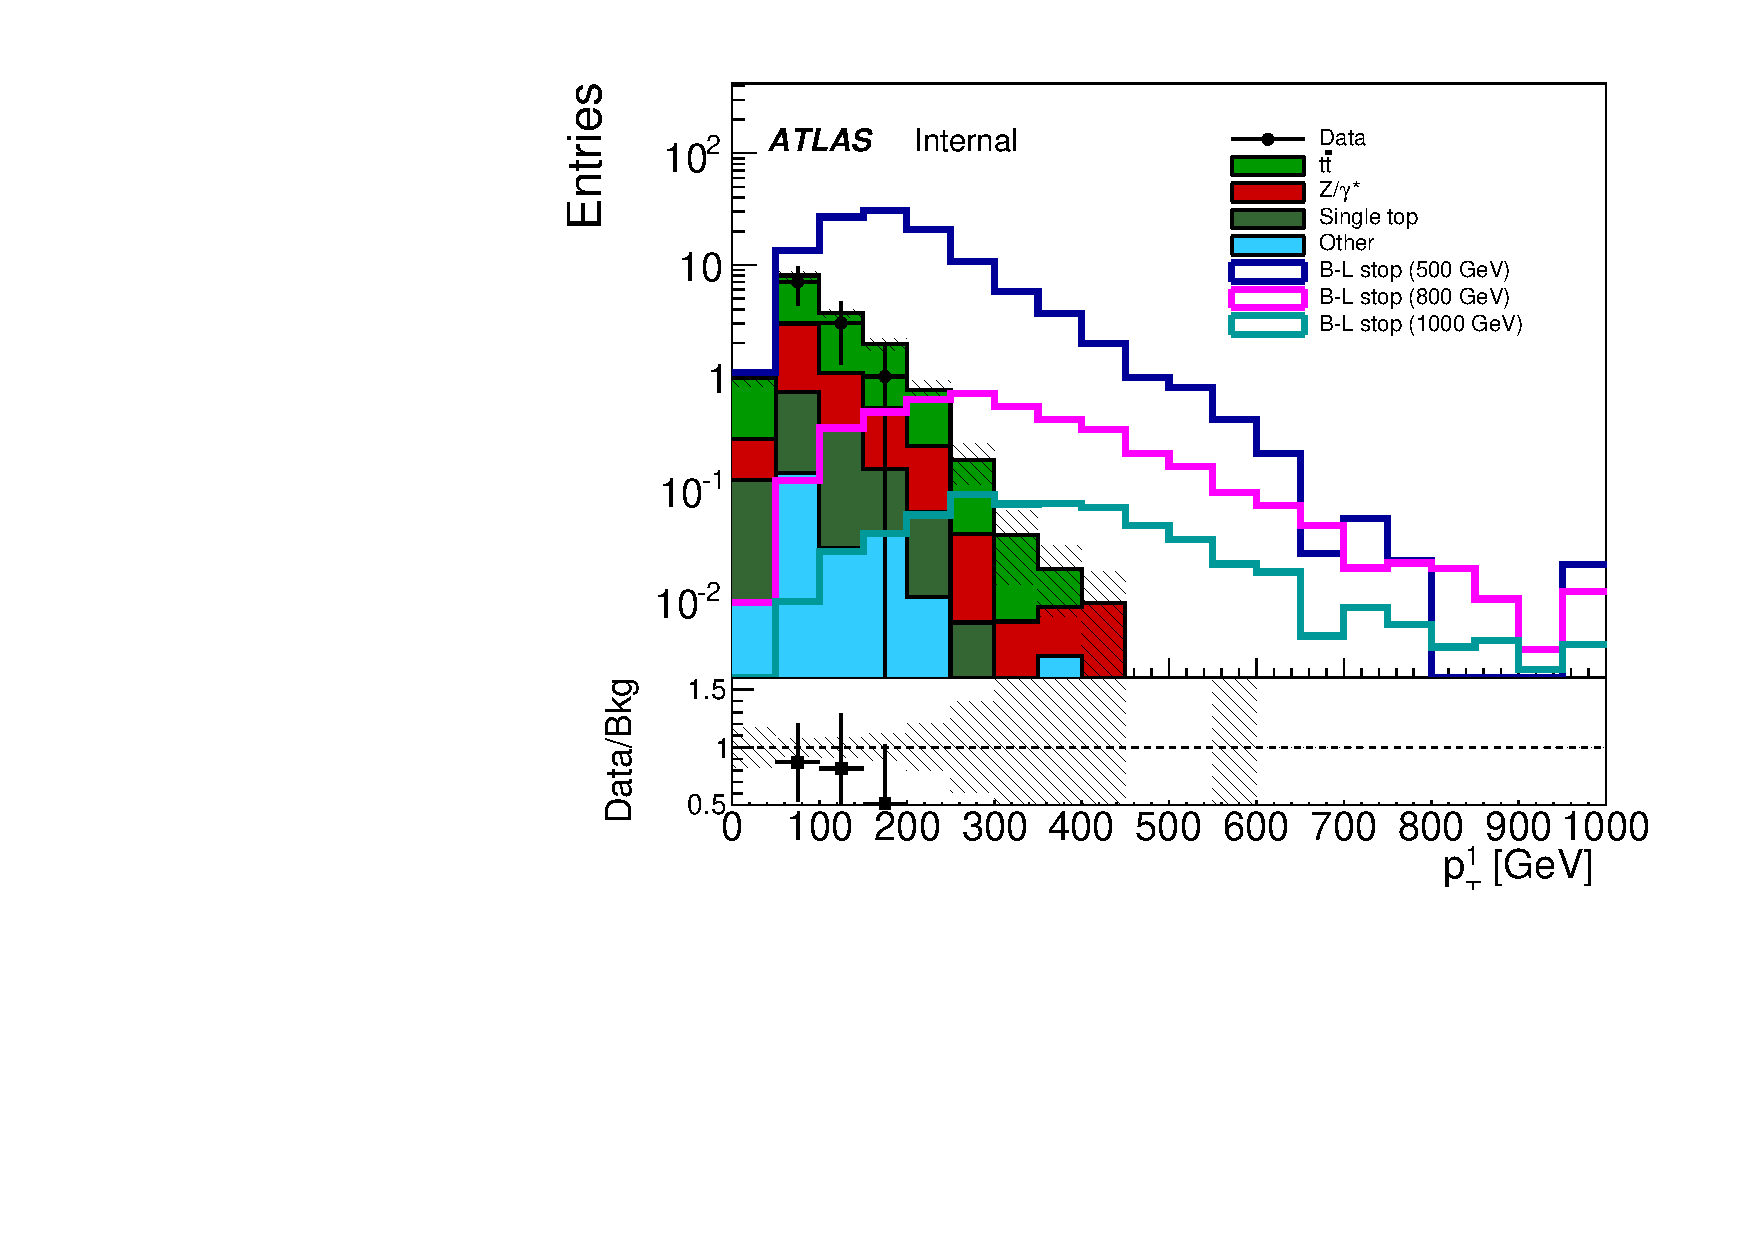
\includegraphics[width=\textwidth]{figures/loose_sr/flavor_ee__lep_pt_1__BMINUSL_SR_HT_1100_MBL_400_MINUS_HT__log.pdf}
%%% %%%     \end{block}
%%% %%%     \column{0.5\textwidth}
%%% %%%     \begin{block}{$\mu\mu$ channel}
%%% %%%       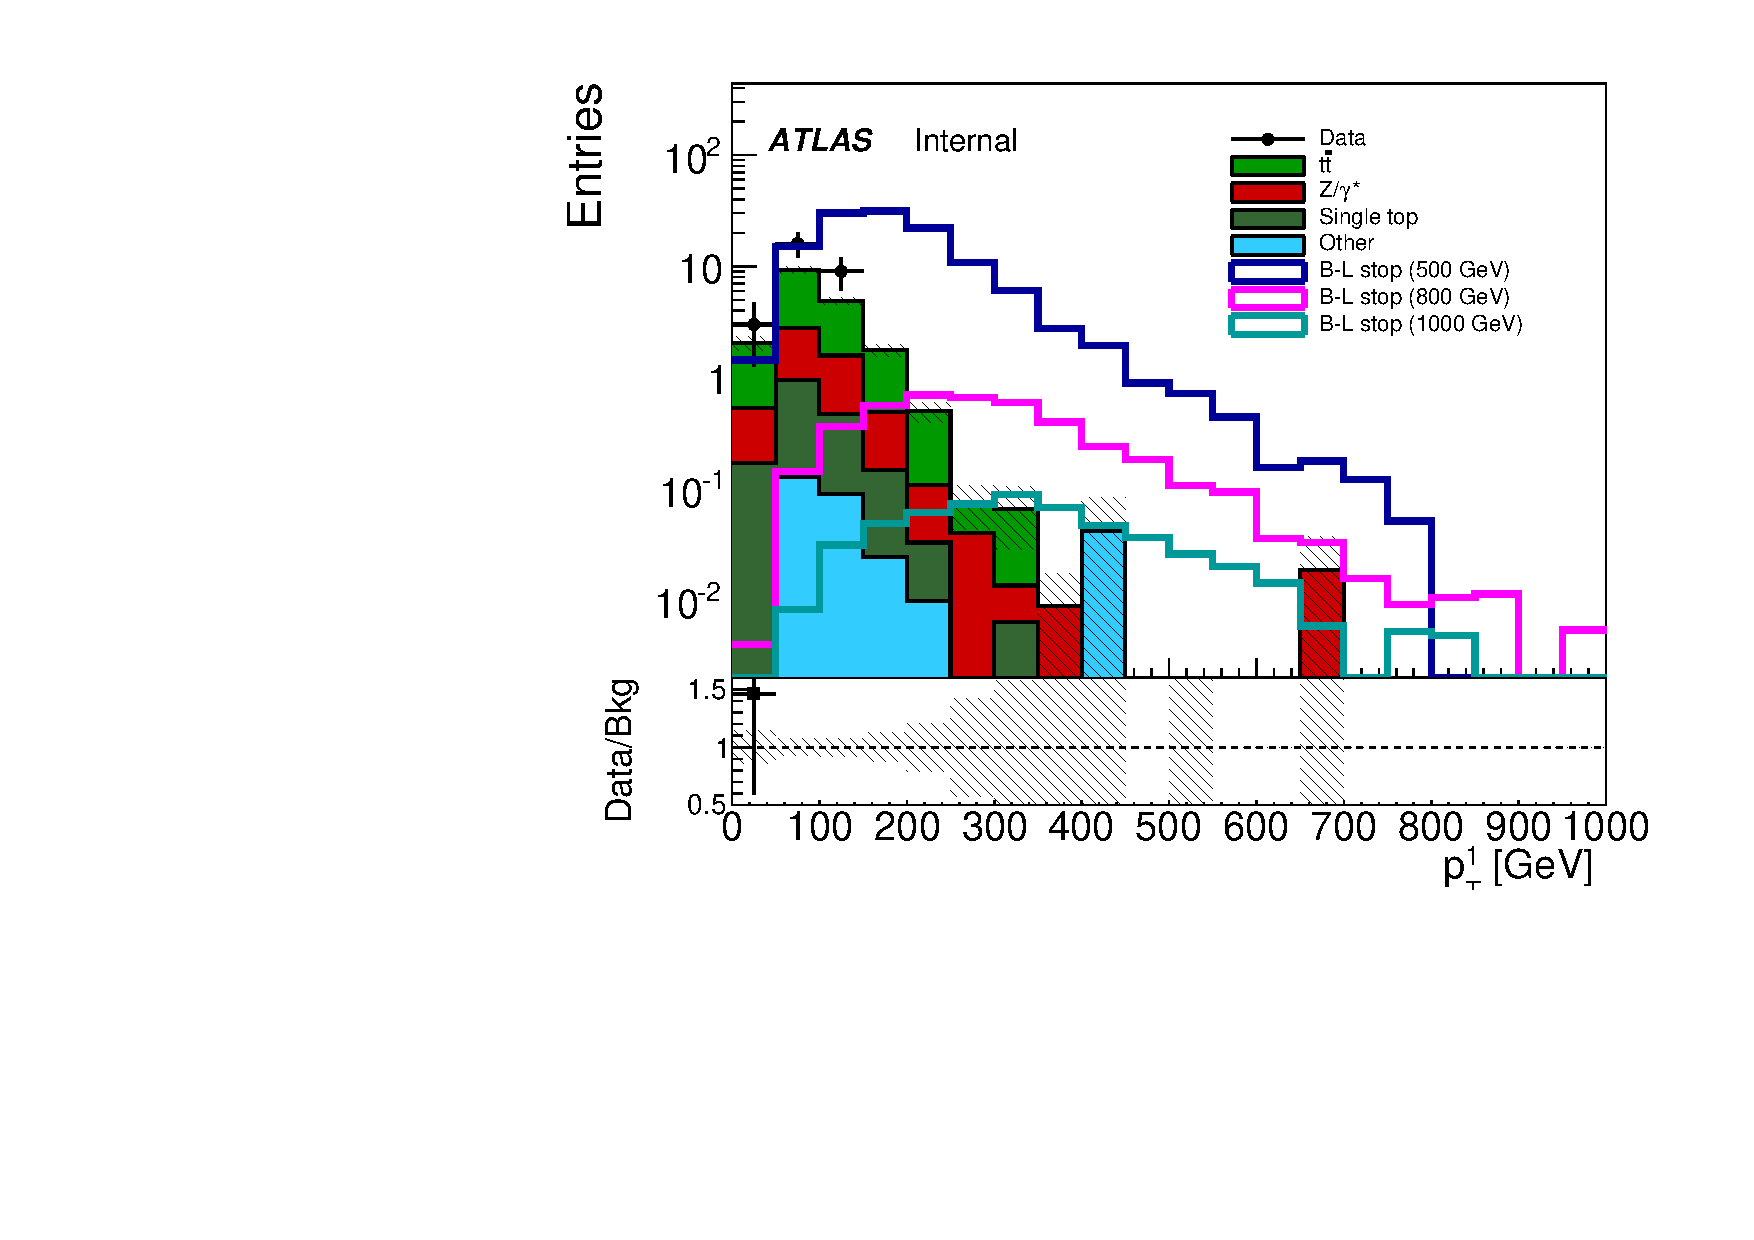
\includegraphics[width=\textwidth]{figures/loose_sr/flavor_mm__lep_pt_1__BMINUSL_SR_HT_1100_MBL_400_MINUS_HT__log.pdf}
%%% %%%     \end{block}
%%% %%%   \end{columns}
%%% %%% \end{frame}
%%% %%% 
%%% %%% 
%%% %%% % ------------------------------------------------------------------------------
%%% %%% \begin{frame}[t]
%%% %%%   {\color{RoyalBlue}
%%% %%%     From SUSY approval: In the looser SR, plot $m_{\ell\ell}$ and
%%% %%%     check for an upper cut.
%%% %%%   }
%%% %%%   \begin{itemize}
%%% %%%     \item There does not seem to be an upper cut  on the $m_{\ell\ell}$ for the
%%% %%%       background samples
%%% %%%   \end{itemize}
%%% %%%   \begin{columns}
%%% %%%     \column{0.5\textwidth}
%%% %%%     \begin{block}{$ee$ channel}
%%% %%%       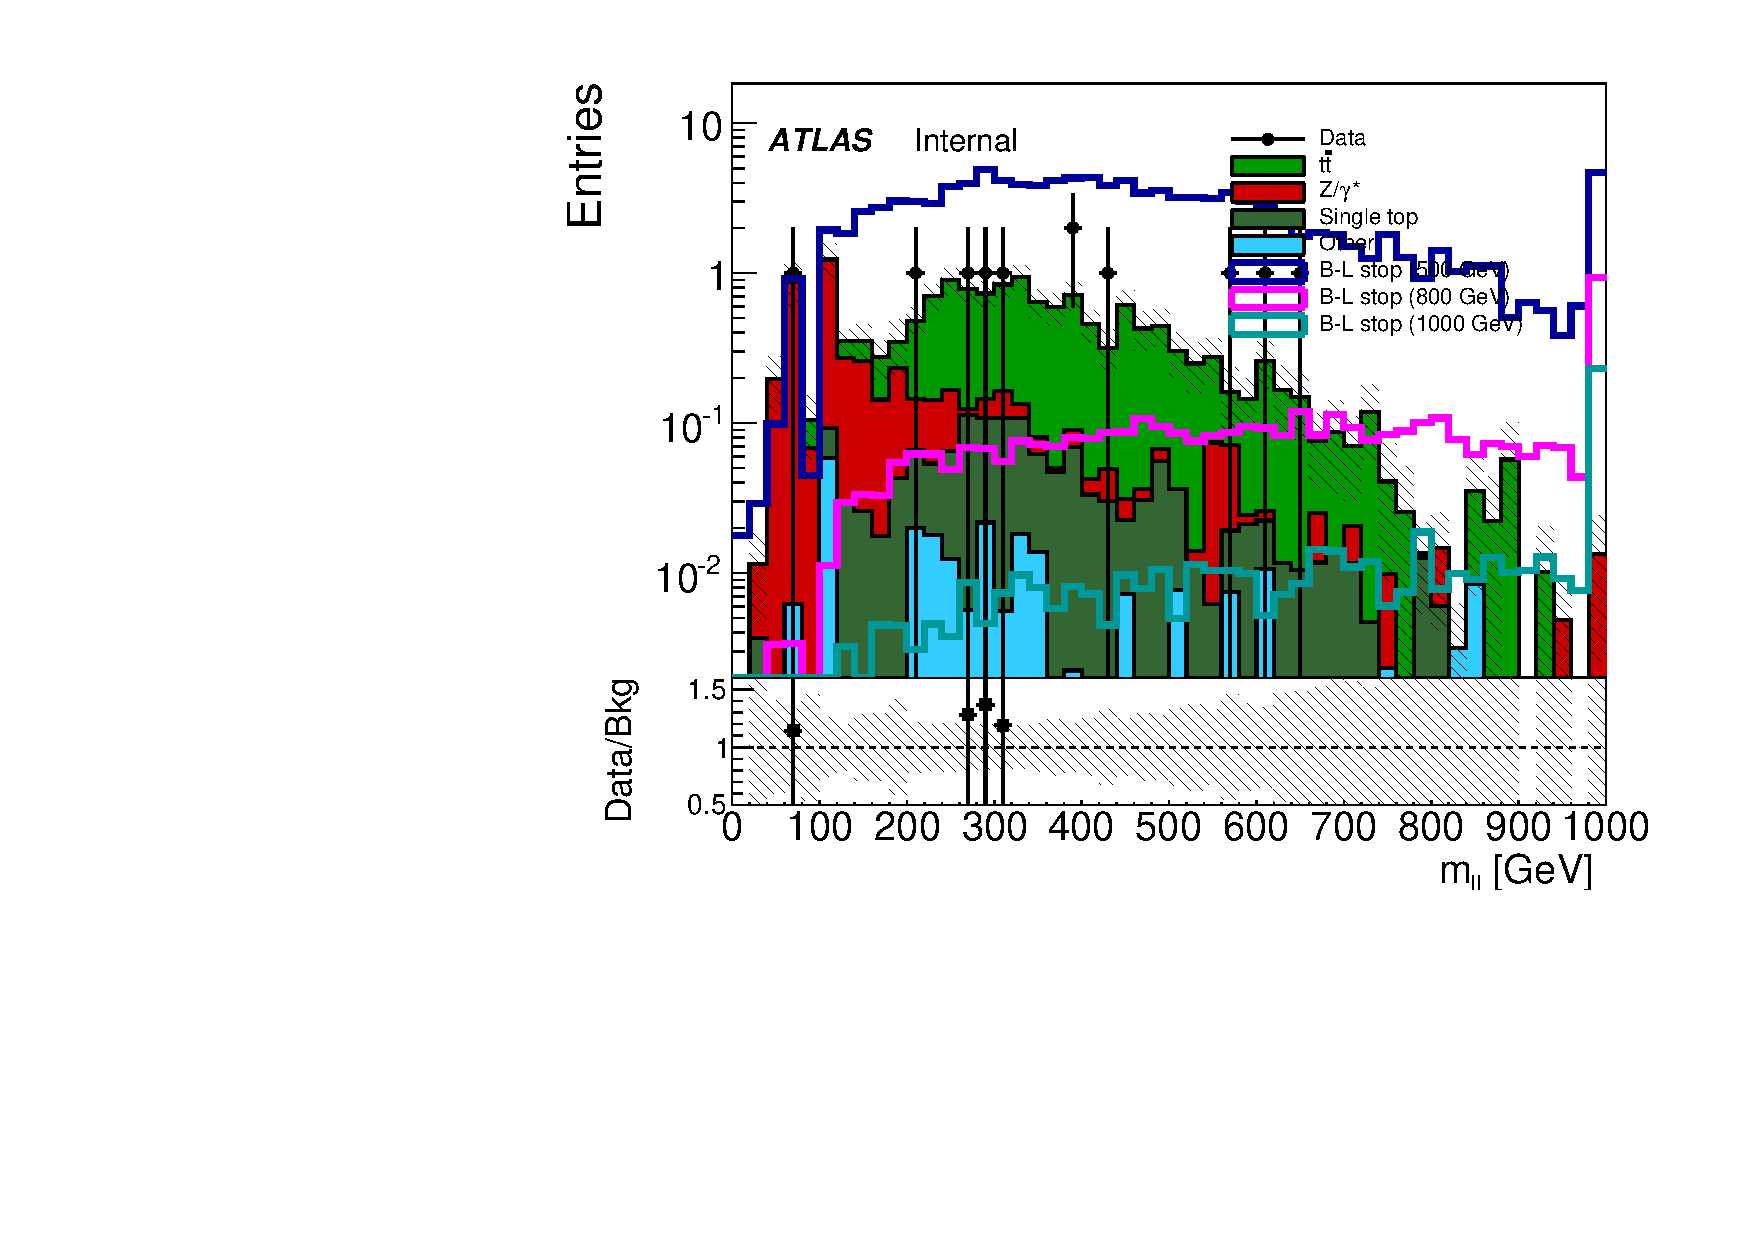
\includegraphics[width=\textwidth]{figures/loose_sr/flavor_ee__mll__BMINUSL_SR_HT_1100_MBL_400_MINUS_HT__log.pdf}
%%% %%%     \end{block}
%%% %%%     \column{0.5\textwidth}
%%% %%%     \begin{block}{$\mu\mu$ channel}
%%% %%%       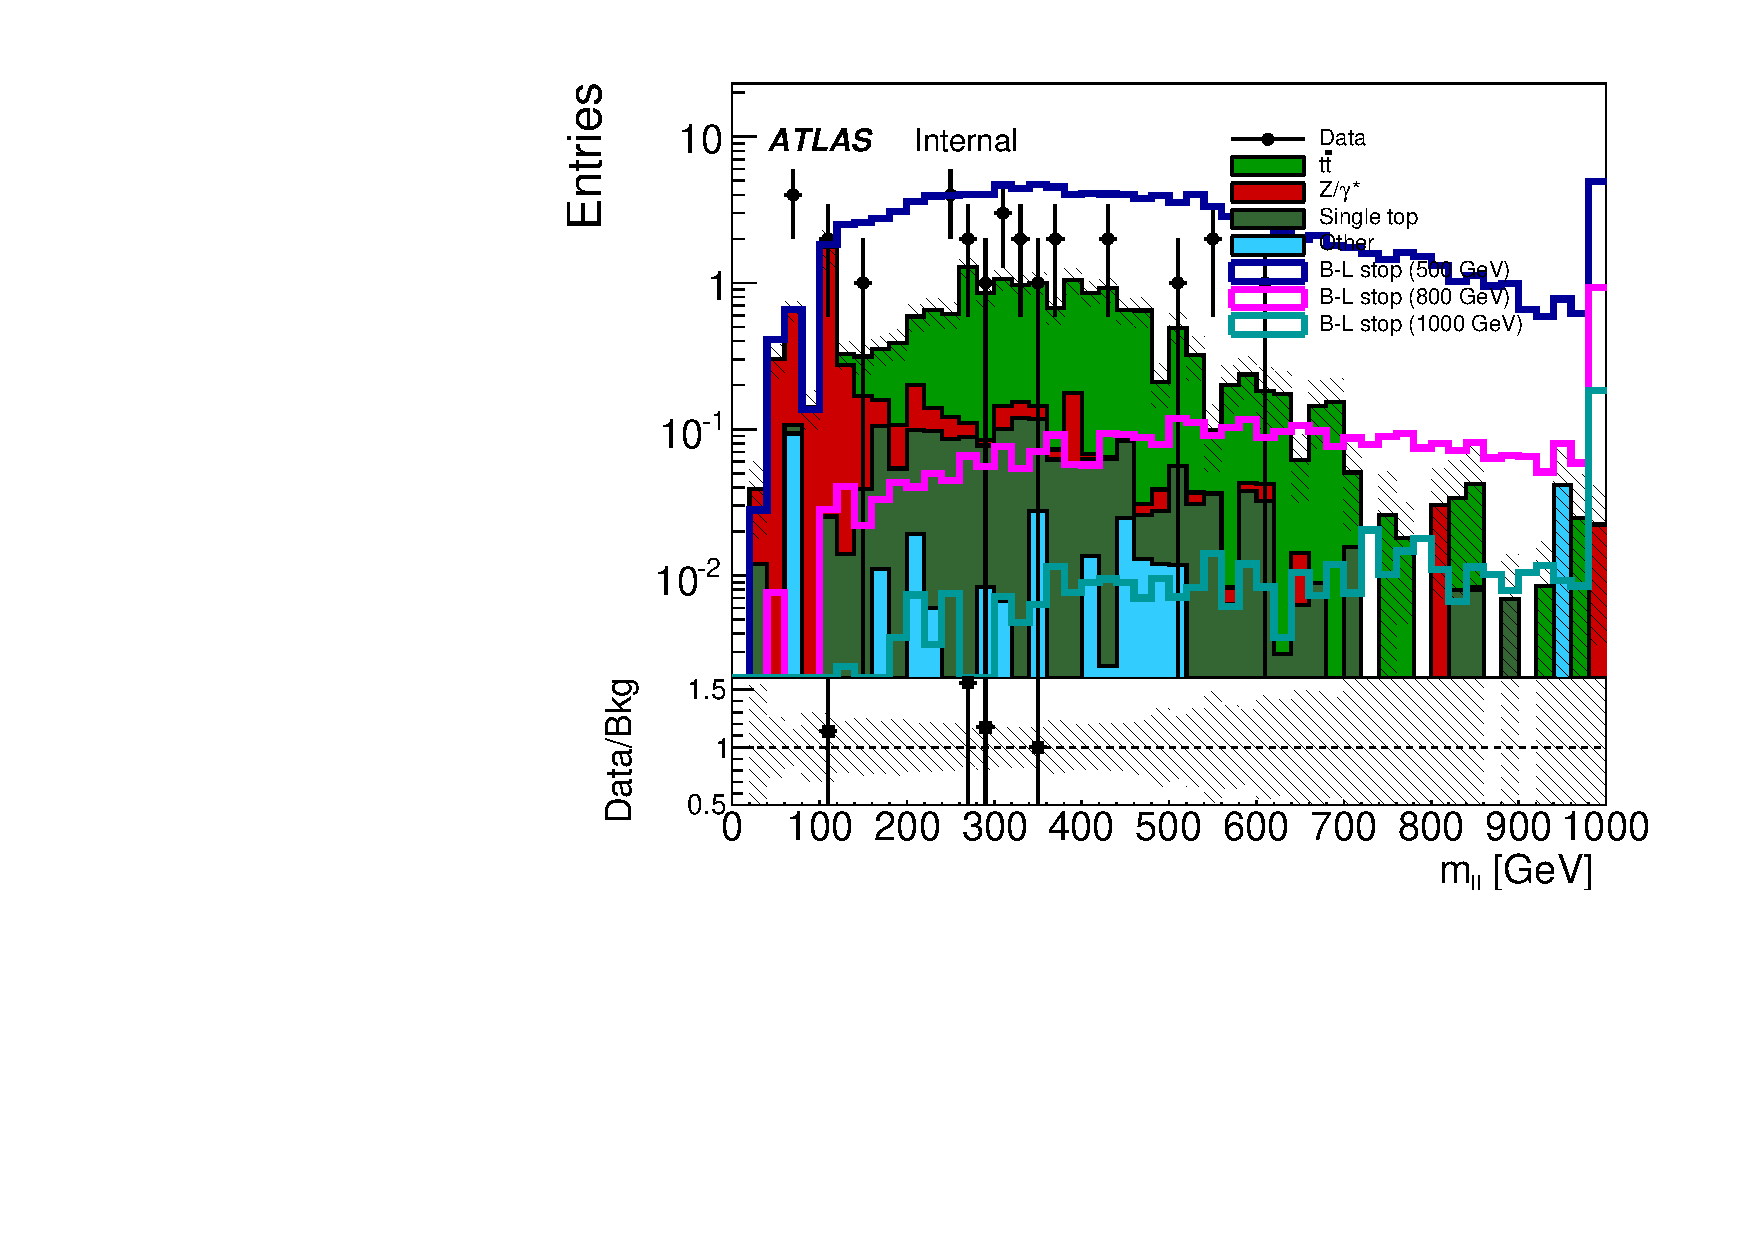
\includegraphics[width=\textwidth]{figures/loose_sr/flavor_mm__mll__BMINUSL_SR_HT_1100_MBL_400_MINUS_HT__log.pdf}
%%% %%%     \end{block}
%%% %%%   \end{columns}
%%% %%% \end{frame}


% ------------------------------------------------------------------------------
\beginbackup


%%% % ------------------------------------------------------------------------------
%%% \begin{frame}
%%%   \begin{center}
%%%     {\Huge \color{RoyalBlue} Backup}
%%%   \end{center}
%%% \end{frame}
%%% 
%%% % ------------------------------------------------------------------------------
%%% \begin{frame}
%%%   \frametitle{Why left-handed stops?}
%%%   \UpdateFlag
%%%   %%
%%% \end{frame}
%%% 
%%% 
%%% %%% 
%%% %%% %% % ------------------------------------------------------------------------------
%%% %%% %% \begin{frame}
%%% %%% %%   \frametitle{Software versions}
%%% %%% %%   \begin{itemize}
%%% %%% %%     \item SUSYTools-00-03-21
%%% %%% %%     \item HistFitter 00-00-39
%%% %%% %%   \end{itemize}
%%% %%% %% \end{frame}
%%% %%% %% 
%%% %%% %% 
%%% %%% %% % ------------------------------------------------------------------------------
%%% %%% %% \begin{frame}
%%% %%% %%   \frametitle{Systematic uncertainty breakdown}
%%% %%% %% 
%%% %%% %%   \begin{columns}
%%% %%% %%     \column{0.5\linewidth}
%%% %%% %%     \begin{block}{Top CR}
%%% %%% %%       \vspace{1ex}
%%% %%% %%       \resizebox{\linewidth}{!}{
%%% %%% %%     \begin{tabular}{l|cccc|c}
%%% %%% %%       \toprule
%%% %%% %%       Systematic                   & $t\bar{t}$ & $Z/\gamma^{*}$ & Single top & Other   & Total   \\
%%% %%% %%       \midrule
%%% %%% %%       Uncertainty (\%)                                                                            \\
%%% %%% %%       \midrule
%%% %%% %%       JES                          & +6/-5      & +3/-9          & +5/-5      & +7/-5   & +6/-5   \\
%%% %%% %%       $b$-tagging                  & +7/-7      & +7/-7          & +7/-7      & +6/-6   & +7/-7   \\
%%% %%% %%       JER                          & 2          & 20             & 0          & 0       & 2       \\
%%% %%% %%       Luminosity                   & -          & -              & 2          & 2       & 0       \\
%%% %%% %%       \midrule
%%% %%% %%       \Ht\ extrapolation           & -          & 0              & -          & -       & 0       \\
%%% %%% %%       MC Statistical               & 0          & 6              & 1          & 4       & 1       \\
%%% %%% %%       % CR Statistical               & 0          & 0              & -          & -       & 0       \\
%%% %%% %%       $Wt$ cross section           & -          & -              & 7          & -       & 0       \\
%%% %%% %%       Renormalization Scale        & 0          & -              & -          & -       & 0       \\
%%% %%% %%       Parton shower                & 0          & -              & -          & -       & 0       \\
%%% %%% %%       Multi-parton                 & -          & 13             & -          & -       & 0       \\
%%% %%% %%       ISR/FSR                      & 0          & -              & 0          & -       & 0       \\
%%% %%% %%       Factorization Scale          & 0          & -              & -          & -       & 0       \\
%%% %%% %%       Interference with $t\bar{t}$ & -          & -              & 0          & -       & 0       \\
%%% %%% %%       \bottomrule
%%% %%% %%     \end{tabular}
%%% %%% %%       }
%%% %%% %%     \end{block}
%%% %%% %%     %%
%%% %%% %%     \column{0.5\linewidth}
%%% %%% %%     \begin{block}{$Z$ CR}
%%% %%% %%       \vspace{1ex}
%%% %%% %%       \resizebox{\linewidth}{!}{
%%% %%% %%     \begin{tabular}{l|cccc|c}
%%% %%% %%       \toprule
%%% %%% %%       Systematic                   & $t\bar{t}$ & $Z/\gamma^{*}$ & Single top & Other   & Total   \\
%%% %%% %%       \midrule
%%% %%% %%       Uncertainty (\%)                                                                            \\
%%% %%% %%       \midrule
%%% %%% %%       JES                          & +2/-2      & +5/-6          & +3/-2      & +5/-4   & +5/-6   \\
%%% %%% %%       $b$-tagging                  & +7/-7      & +8/-7          & +7/-7      & +7/-7   & +8/-7   \\
%%% %%% %%       JER                          & 0          & 2              & 4          & 1       & 2       \\
%%% %%% %%       Luminosity                   & -          & -              & 2          & 2       & 0       \\
%%% %%% %%       \midrule
%%% %%% %%       \Ht\ extrapolation           & -          & 0              & -          & -       & 0       \\
%%% %%% %%       MC Statistical               & 0          & 0              & 2          & 2       & 0       \\
%%% %%% %%       % CR Statistical               & 0          & 0              & -          & -       & 0       \\
%%% %%% %%       $Wt$ cross section           & -          & -              & 7          & -       & 0       \\
%%% %%% %%       Renormalization Scale        & 0          & -              & -          & -       & 0       \\
%%% %%% %%       Parton shower                & 0          & -              & -          & -       & 0       \\
%%% %%% %%       Multi-parton                 & -          & 0              & -          & -       & 0       \\
%%% %%% %%       ISR/FSR                      & 0          & -              & 0          & -       & 0       \\
%%% %%% %%       Factorization Scale          & 0          & -              & -          & -       & 0       \\
%%% %%% %%       Interference with $t\bar{t}$ & -          & -              & 0          & -       & 0       \\
%%% %%% %%       \bottomrule
%%% %%% %%     \end{tabular}
%%% %%% %%       }
%%% %%% %%     \end{block}
%%% %%% %%   \end{columns}
%%% %%% %% \end{frame}
%%% %%% %% 
%%% %%% %% 
%%% %%% %% % ------------------------------------------------------------------------------
%%% %%% %% \begin{frame}
%%% %%% %%   \frametitle{Systematic uncertainty breakdown}
%%% %%% %% 
%%% %%% %%   \begin{columns}
%%% %%% %%     \column{0.5\linewidth}
%%% %%% %%     \begin{block}{Top VR 1}
%%% %%% %%       \vspace{1ex}
%%% %%% %%       \resizebox{\linewidth}{!}{
%%% %%% %%     \begin{tabular}{l|cccc|c}
%%% %%% %%       \toprule
%%% %%% %%       Systematic                   & $t\bar{t}$ & $Z/\gamma^{*}$ & Single top & Other   & Total   \\
%%% %%% %%       \midrule
%%% %%% %%       Uncertainty (\%)                                                                            \\
%%% %%% %%       \midrule
%%% %%% %%       JES                          & +2/-2      & +3/-6          & +3/-3      & +2/-5   & +3/-3   \\
%%% %%% %%       $b$-tagging                  & +7/-7      & +8/-8          & +7/-7      & +7/-7   & +7/-7   \\
%%% %%% %%       JER                          & 0          & 4              & 0          & 2       & 0       \\
%%% %%% %%       Luminosity                   & -          & -              & 2          & 2       & 0       \\
%%% %%% %%       \midrule
%%% %%% %%       \Ht\ extrapolation           & -          & 0              & -          & -       & 0       \\
%%% %%% %%       MC Statistical               & 0          & 2              & 1          & 4       & 0       \\
%%% %%% %%       % CR Statistical               & 0          & 0              & -          & -       & 0       \\
%%% %%% %%       $Wt$ cross section           & -          & -              & 7          & -       & 0       \\
%%% %%% %%       Renormalization Scale        & 0          & -              & -          & -       & 0       \\
%%% %%% %%       Parton shower                & 0          & -              & -          & -       & 0       \\
%%% %%% %%       Multi-parton                 & -          & 13             & -          & -       & 1       \\
%%% %%% %%       ISR/FSR                      & 0          & -              & 0          & -       & 0       \\
%%% %%% %%       Factorization Scale          & 0          & -              & -          & -       & 0       \\
%%% %%% %%       Interference with $t\bar{t}$ & -          & -              & 0          & -       & 0       \\
%%% %%% %%       \bottomrule
%%% %%% %%     \end{tabular}
%%% %%% %%       }
%%% %%% %%     \end{block}
%%% %%% %%     %%
%%% %%% %%     \column{0.5\linewidth}
%%% %%% %%     \begin{block}{Top VR 2}
%%% %%% %%       \vspace{1ex}
%%% %%% %%       \resizebox{\linewidth}{!}{
%%% %%% %%         \begin{tabular}{l|cccc|c}
%%% %%% %%           \toprule
%%% %%% %%           Systematic                   & $t\bar{t}$ & $Z/\gamma^{*}$ & Single top & Other   & Total   \\
%%% %%% %%           \midrule
%%% %%% %%           Uncertainty (\%)                                                                            \\
%%% %%% %%           \midrule
%%% %%% %%           JES                          & +3/-3      & +8/-2          & +2/-4      & +9/-1   & +3/-3   \\
%%% %%% %%           $b$-tagging                  & +6/-6      & +10/-9         & +7/-7      & +7/-7   & +7/-7   \\
%%% %%% %%           JER                          & 1          & 2              & 0          & 13      & 1       \\
%%% %%% %%           Luminosity                   & -          & -              & 2          & 2       & 0       \\
%%% %%% %%           \midrule
%%% %%% %%           \Ht\ extrapolation           & -          & 0              & -          & -       & 0       \\
%%% %%% %%           MC Statistical               & 0          & 2              & 0          & 2       & 0       \\
%%% %%% %%           % CR Statistical               & 0          & 0              & -          & -       & 0       \\
%%% %%% %%           $Wt$ cross section           & -          & -              & 7          & -       & 0       \\
%%% %%% %%           Renormalization Scale        & 0          & -              & -          & -       & 0       \\
%%% %%% %%           Parton shower                & 0          & -              & -          & -       & 0       \\
%%% %%% %%           Multi-parton                 & -          & 0              & -          & -       & 0       \\
%%% %%% %%           ISR/FSR                      & 0          & -              & 0          & -       & 0       \\
%%% %%% %%           Factorization Scale          & 0          & -              & -          & -       & 0       \\
%%% %%% %%           Interference with $t\bar{t}$ & -          & -              & 0          & -       & 0       \\
%%% %%% %%           \bottomrule
%%% %%% %%         \end{tabular}
%%% %%% %%       }
%%% %%% %%     \end{block}
%%% %%% %%   \end{columns}
%%% %%% %% \end{frame}
%%% %%% %% 
%%% %%% %% 
%%% %%% %% % ------------------------------------------------------------------------------
%%% %%% %% \begin{frame}
%%% %%% %%   \frametitle{Systematic uncertainty breakdown}
%%% %%% %% 
%%% %%% %%   \begin{columns}
%%% %%% %%     \column{0.5\linewidth}
%%% %%% %%     \begin{block}{Top VR 3}
%%% %%% %%       \vspace{1ex}
%%% %%% %%       \resizebox{\linewidth}{!}{
%%% %%% %%     \begin{tabular}{l|cccc|c}
%%% %%% %%       \toprule
%%% %%% %%       Systematic                   & $t\bar{t}$ & $Z/\gamma^{*}$ & Single top & Other   & Total   \\
%%% %%% %%       \midrule
%%% %%% %%       Uncertainty (\%)                                                                            \\
%%% %%% %%       \midrule
%%% %%% %%       JES                          & +7/-6      & +12/-2         & +7/-4      & +11/-7  & +7/-6   \\
%%% %%% %%       $b$-tagging                  & +8/-8      & +10/-9         & +9/-8      & +8/-8   & +8/-8   \\
%%% %%% %%       JER                          & 1          & 6              & 0          & 1       & 1       \\
%%% %%% %%       Luminosity                   & -          & -              & 2          & 2       & 0       \\
%%% %%% %%       \midrule
%%% %%% %%       \Ht\ extrapolation           & -          & 50             & -          & -       & 1       \\
%%% %%% %%       MC Statistical               & 2          & 4              & 1          & 5       & 2       \\
%%% %%% %%       % CR Statistical               & 0          & 0              & -          & -       & 0       \\
%%% %%% %%       $Wt$ cross section           & -          & -              & 7          & -       & 1       \\
%%% %%% %%       Renormalization Scale        & 0          & -              & -          & -       & 0       \\
%%% %%% %%       Parton shower                & 0          & -              & -          & -       & 0       \\
%%% %%% %%       Multi-parton                 & -          & 0              & -          & -       & 0       \\
%%% %%% %%       ISR/FSR                      & 0          & -              & 0          & -       & 0       \\
%%% %%% %%       Factorization Scale          & 0          & -              & -          & -       & 0       \\
%%% %%% %%       Interference with $t\bar{t}$ & -          & -              & 0          & -       & 0       \\
%%% %%% %%       \bottomrule
%%% %%% %%     \end{tabular}
%%% %%% %%       }
%%% %%% %%     \end{block}
%%% %%% %%     %%
%%% %%% %%     \column{0.5\linewidth}
%%% %%% %%     \begin{block}{$Z$ VR}
%%% %%% %%       \vspace{1ex}
%%% %%% %%       \resizebox{\linewidth}{!}{
%%% %%% %%     \begin{tabular}{l|cccc|c}
%%% %%% %%       \toprule
%%% %%% %%       Systematic                   & $t\bar{t}$ & $Z/\gamma^{*}$ & Single top & Other   & Total   \\
%%% %%% %%       \midrule
%%% %%% %%       Uncertainty (\%)                                                                            \\
%%% %%% %%       \midrule
%%% %%% %%       JES                          & +6/-11     & +4/-5          & +5/-5      & +3/-2   & +4/-5   \\
%%% %%% %%       $b$-tagging                  & +10/-10    & +11/-11        & +9/-9      & +9/-9   & +11/-11 \\
%%% %%% %%       JER                          & 1          & 0              & 3          & 2       & 0       \\
%%% %%% %%       Luminosity                   & -          & -              & 2          & 2       & 0       \\
%%% %%% %%       \midrule
%%% %%% %%       \Ht\ extrapolation           & -          & 50             & -          & -       & 46      \\
%%% %%% %%       MC Statistical               & 8          & 0              & 11         & 4       & 1       \\
%%% %%% %%       % CR Statistical               & 0          & 0              & -          & -       & 0       \\
%%% %%% %%       $Wt$ cross section           & -          & -              & 7          & -       & 0       \\
%%% %%% %%       Renormalization Scale        & 2          & -              & -          & -       & 0       \\
%%% %%% %%       Parton shower                & 11         & -              & -          & -       & 0       \\
%%% %%% %%       Multi-parton                 & -          & 13             & -          & -       & 12      \\
%%% %%% %%       ISR/FSR                      & 6          & -              & 0          & -       & 0       \\
%%% %%% %%       Factorization Scale          & 1          & -              & -          & -       & 0       \\
%%% %%% %%       Interference with $t\bar{t}$ & -          & -              & 9          & -       & 0       \\
%%% %%% %%       \bottomrule
%%% %%% %%     \end{tabular}
%%% %%% %%       }
%%% %%% %%     \end{block}
%%% %%% %%   \end{columns}
%%% %%% %% \end{frame}
%%% %%% %% 
%%% %%% %% 
%%% %%% %% % ------------------------------------------------------------------------------
%%% %%% %% \begin{frame}
%%% %%% %%   \frametitle{Top validation region 1}
%%% %%% %%   %%
%%% %%% %%   \begin{columns}
%%% %%% %%     \column{0.45\textwidth}
%%% %%% %%     \begin{block}{\Ht}
%%% %%% %%       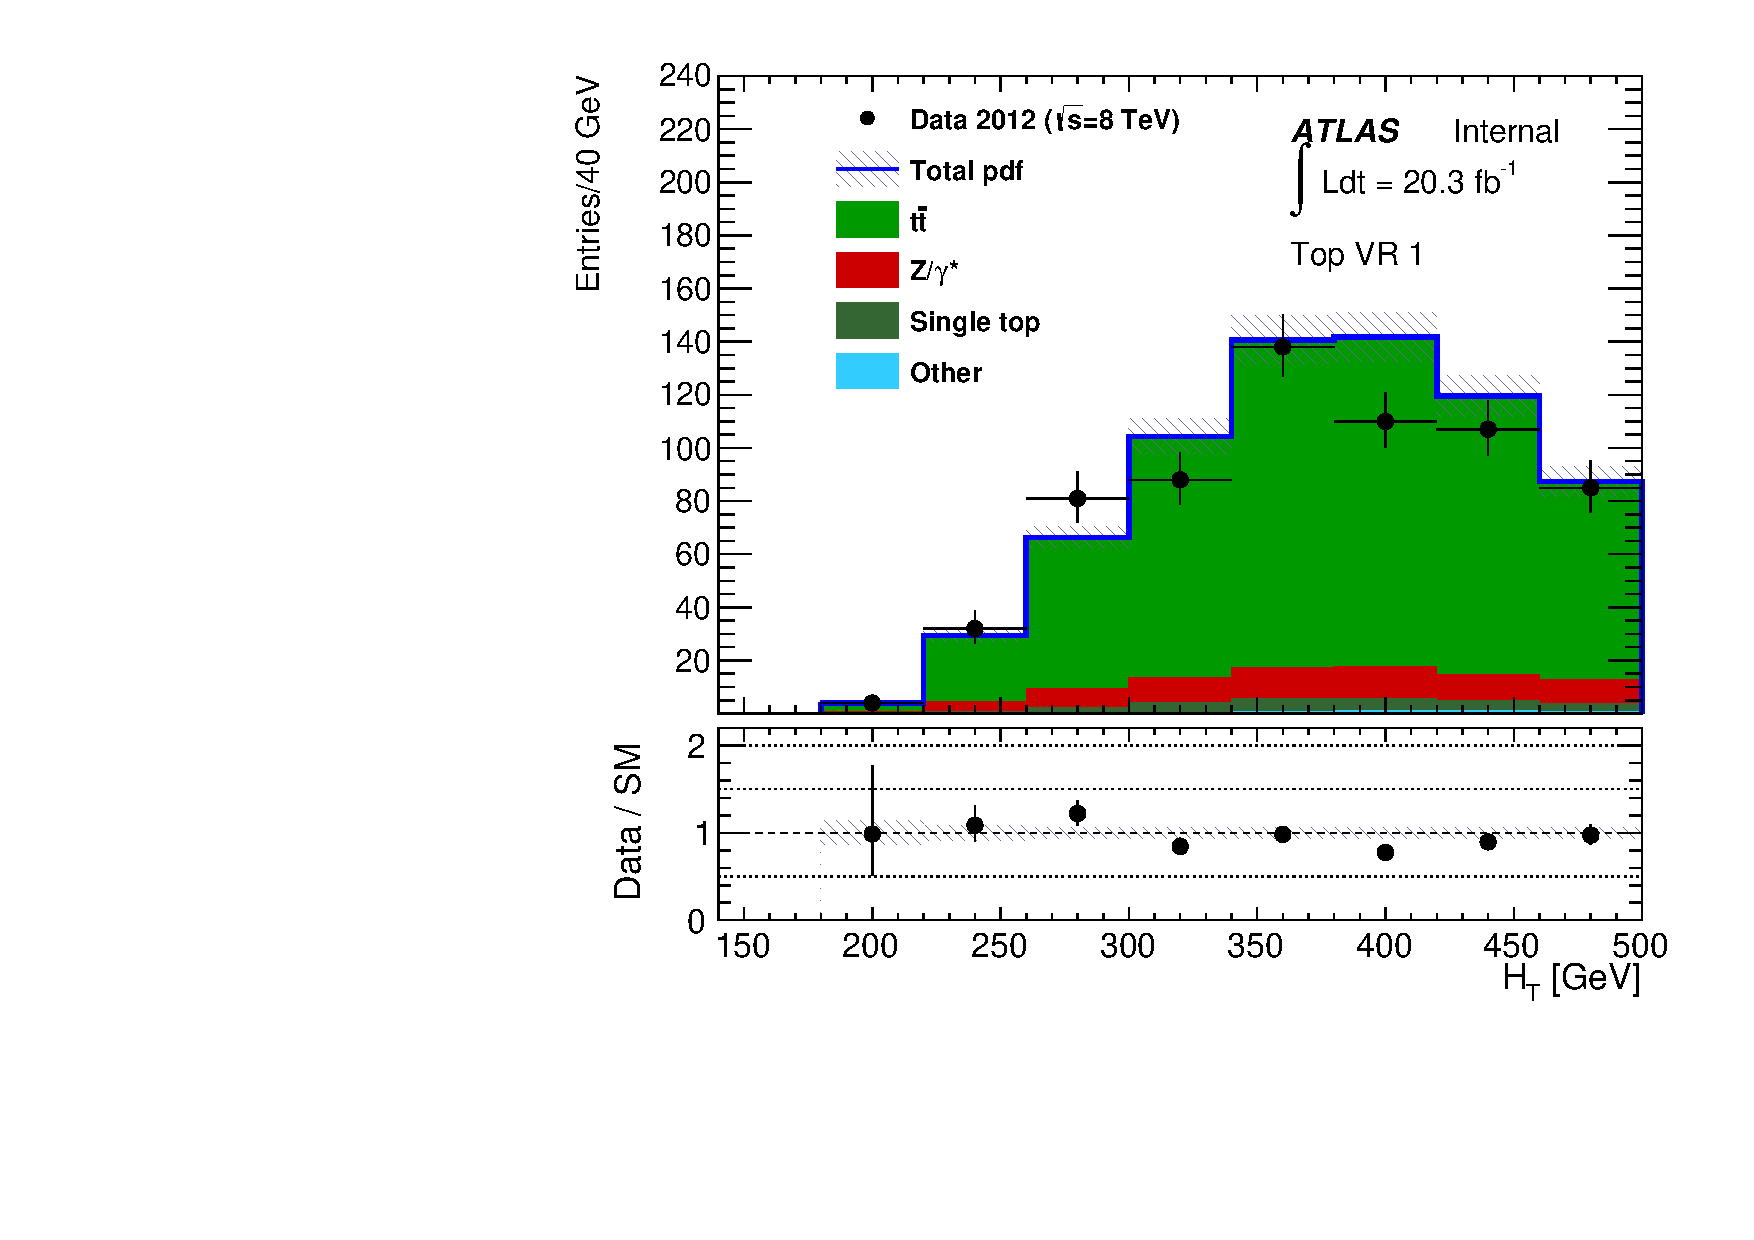
\includegraphics[width=\textwidth]{figures/vr_top_1_ht_signal.pdf}
%%% %%% %%     \end{block}
%%% %%% %%     \column{0.45\textwidth}
%%% %%% %%     \begin{block}{\Mbl}
%%% %%% %%       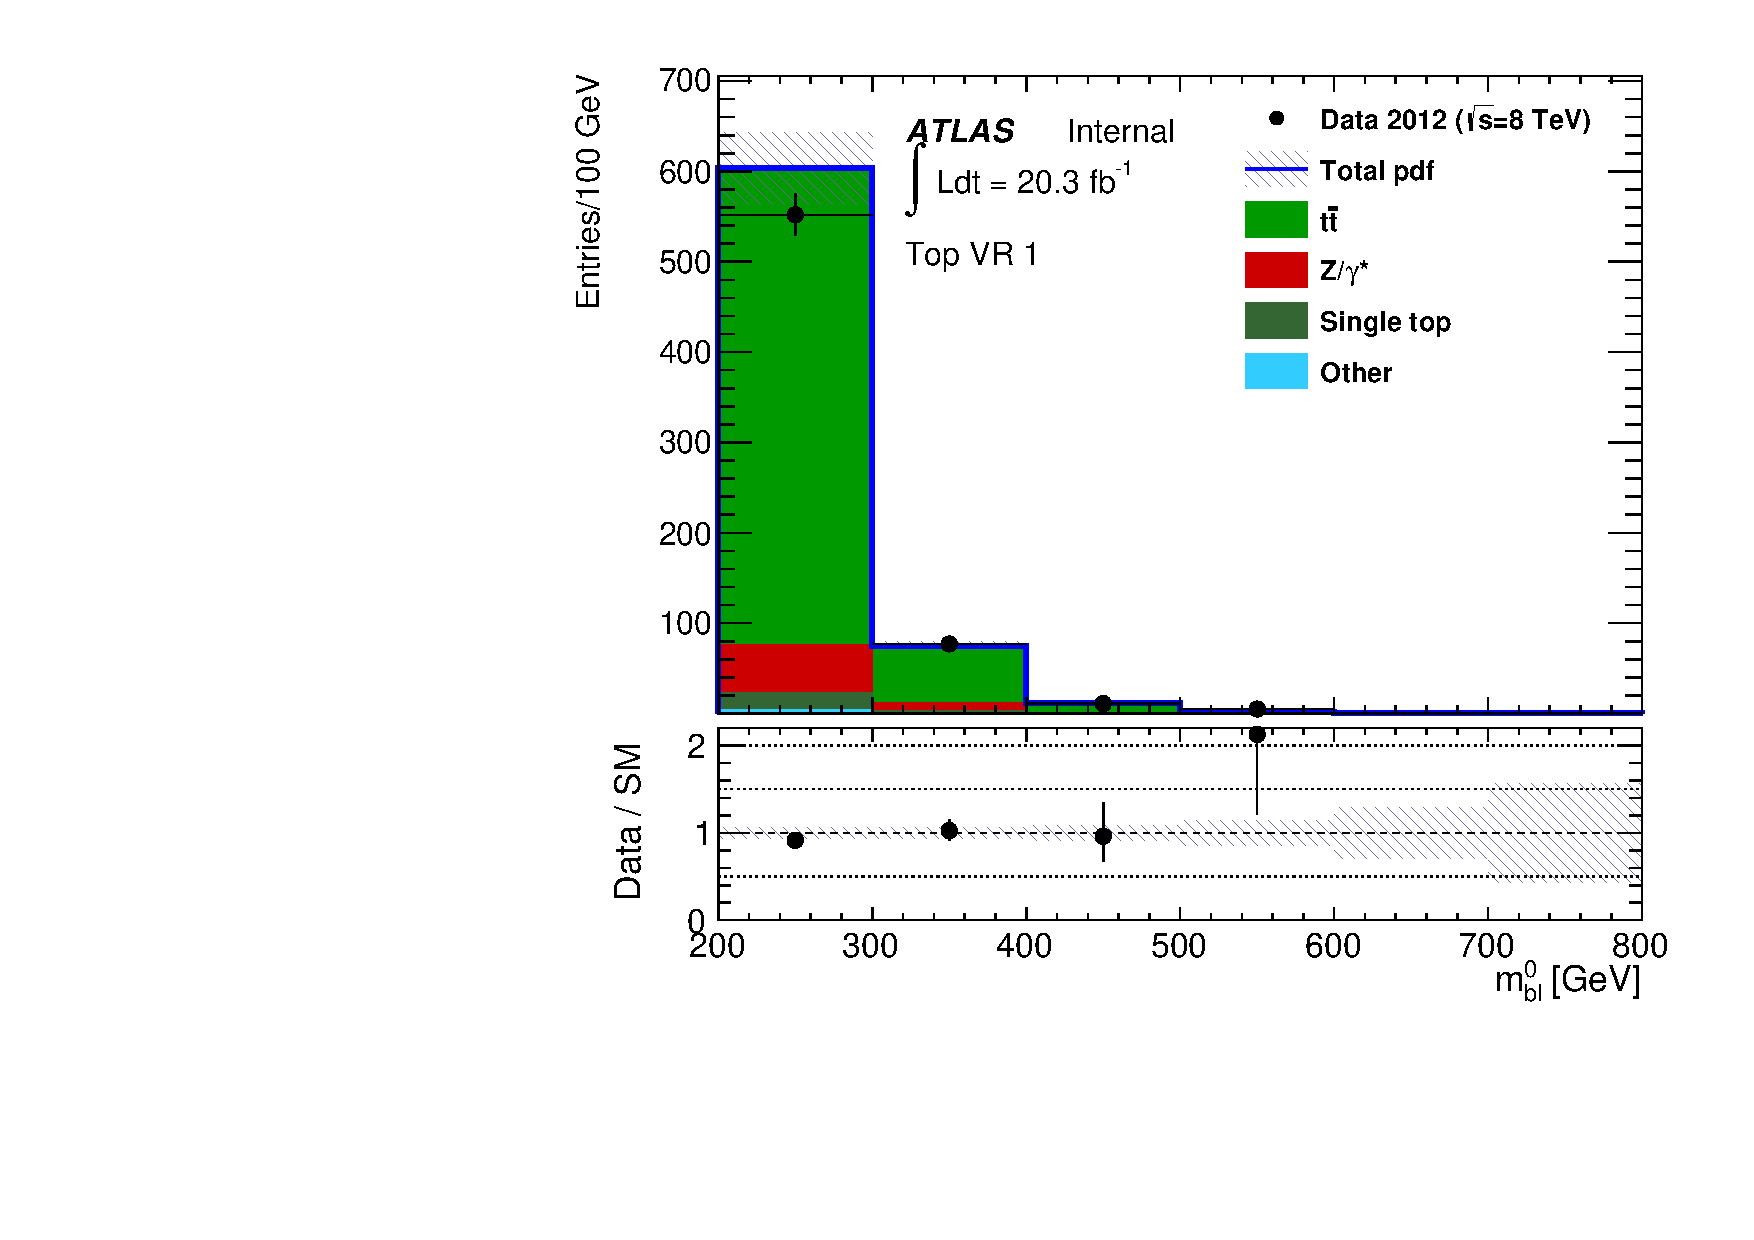
\includegraphics[width=\textwidth]{figures/vr_top_1_mbl_0.pdf}
%%% %%% %%     \end{block}
%%% %%% %%   \end{columns}
%%% %%% %%   %%
%%% %%% %%   \begin{itemize}
%%% %%% %%     \item Good agreement in top VR 1
%%% %%% %%   \end{itemize}
%%% %%% %% \end{frame}
%%% %%% %% 
%%% %%% %% 
%%% %%% %% % ------------------------------------------------------------------------------
%%% %%% %% \begin{frame}
%%% %%% %%   \frametitle{Top validation region 2}
%%% %%% %%   %%
%%% %%% %%   \begin{columns}
%%% %%% %%     \column{0.45\textwidth}
%%% %%% %%     \begin{block}{\Ht}
%%% %%% %%       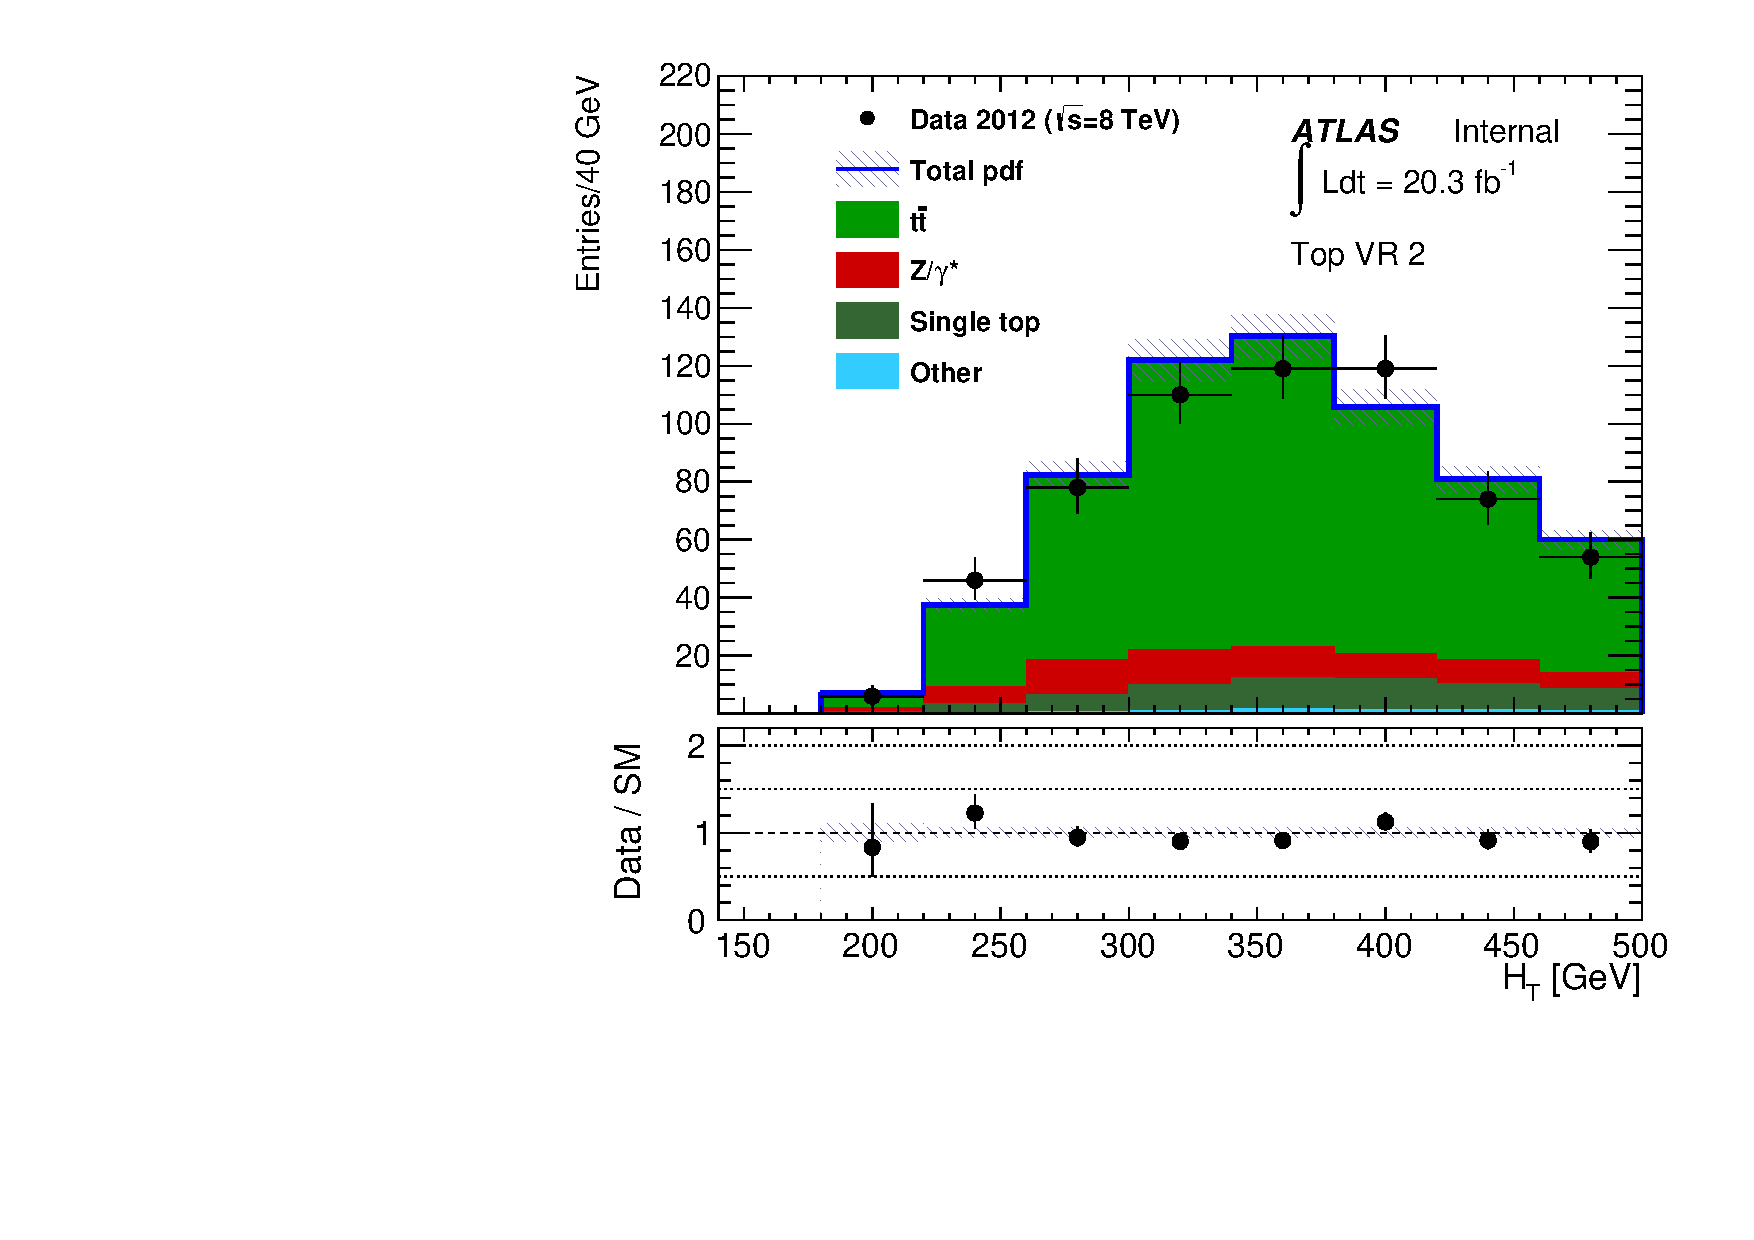
\includegraphics[width=\textwidth]{figures/vr_top_2_ht_signal.pdf}
%%% %%% %%     \end{block}
%%% %%% %%     \column{0.45\textwidth}
%%% %%% %%     \begin{block}{\Mbl}
%%% %%% %%       \includegraphics[width=\textwidth]{figures/vr_top_2_mbl_0.pdf}
%%% %%% %%     \end{block}
%%% %%% %%   \end{columns}
%%% %%% %%   %%
%%% %%% %%   \begin{itemize}
%%% %%% %%     \item Good agreement in top VR 2
%%% %%% %%   \end{itemize}
%%% %%% %% \end{frame}
%%% %%% %% 
%%% %%% %% 
%%% %%% %% % ------------------------------------------------------------------------------
%%% %%% %% \begin{frame}
%%% %%% %%   \includegraphics[width=\textwidth]{figures/event_display_run_210302_event_2292645761.pdf}
%%% %%% %% \end{frame}
%%% %%% %% 
%%% %%% %% 
%%% %%% %% % ------------------------------------------------------------------------------
%%% %%% %% \begin{frame}
%%% %%% %%   \includegraphics[width=\textwidth]{figures/event_display_run_214216_event_121272046.pdf}
%%% %%% %% \end{frame}
%%% %%% %% 
%%% %%% %% 
%%% %%% %% % ------------------------------------------------------------------------------
%%% %%% %% \begin{frame}[t]
%%% %%% %%   \frametitle{Expected $CL_S$: $m_{\tilde{t}}$ = 400 GeV}
%%% %%% %%   \begin{columns}
%%% %%% %%     \column{0.50\textwidth}
%%% %%% %%     \begin{block}{SR 400}
%%% %%% %%       \includegraphics[width=0.8\textwidth]{figures/cls_plots/cls_vs_br_m_400_sr_400_exp.pdf}
%%% %%% %%     \end{block}
%%% %%% %%     \column{0.50\textwidth}
%%% %%% %%     \begin{block}{SR 600}
%%% %%% %%       \includegraphics[width=0.8\textwidth]{figures/cls_plots/cls_vs_br_m_400_sr_600_exp.pdf}
%%% %%% %%     \end{block}
%%% %%% %%   \end{columns}
%%% %%% %%   %
%%% %%% %%   \begin{center}
%%% %%% %%     \begin{minipage}{4cm}
%%% %%% %%       \begin{block}{Region choice}
%%% %%% %%       \includegraphics[width=\textwidth]{figures/cls_plots/region_choice_vs_br_m_400.pdf}
%%% %%% %%       \end{block}
%%% %%% %%     \end{minipage}
%%% %%% %%   \end{center}
%%% %%% %% 
%%% %%% %% \end{frame}
%%% %%% %% 
%%% %%% %% 
%%% %%% %% % ------------------------------------------------------------------------------
%%% %%% %% \begin{frame}[t]
%%% %%% %%   \frametitle{Expected $CL_S$: $m_{\tilde{t}}$ = 500 GeV}
%%% %%% %%   \begin{columns}
%%% %%% %%     \column{0.50\textwidth}
%%% %%% %%     \begin{block}{SR 400}
%%% %%% %%       \includegraphics[width=0.8\textwidth]{figures/cls_plots/cls_vs_br_m_500_sr_400_exp.pdf}
%%% %%% %%     \end{block}
%%% %%% %%     \column{0.50\textwidth}
%%% %%% %%     \begin{block}{SR 600}
%%% %%% %%       \includegraphics[width=0.8\textwidth]{figures/cls_plots/cls_vs_br_m_500_sr_600_exp.pdf}
%%% %%% %%     \end{block}
%%% %%% %%   \end{columns}
%%% %%% %%   %
%%% %%% %%   \begin{center}
%%% %%% %%     \begin{minipage}{4cm}
%%% %%% %%       \begin{block}{Region choice}
%%% %%% %%       \includegraphics[width=\textwidth]{figures/cls_plots/region_choice_vs_br_m_500.pdf}
%%% %%% %%       \end{block}
%%% %%% %%     \end{minipage}
%%% %%% %%   \end{center}
%%% %%% %% 
%%% %%% %% \end{frame}
%%% %%% %% 
%%% %%% %% 
%%% %%% %% % ------------------------------------------------------------------------------
%%% %%% %% \begin{frame}[t]
%%% %%% %%   \frametitle{Expected $CL_S$: $m_{\tilde{t}}$ = 600 GeV}
%%% %%% %%   \begin{columns}
%%% %%% %%     \column{0.50\textwidth}
%%% %%% %%     \begin{block}{SR 400}
%%% %%% %%       \includegraphics[width=0.8\textwidth]{figures/cls_plots/cls_vs_br_m_600_sr_400_exp.pdf}
%%% %%% %%     \end{block}
%%% %%% %%     \column{0.50\textwidth}
%%% %%% %%     \begin{block}{SR 600}
%%% %%% %%       \includegraphics[width=0.8\textwidth]{figures/cls_plots/cls_vs_br_m_600_sr_600_exp.pdf}
%%% %%% %%     \end{block}
%%% %%% %%   \end{columns}
%%% %%% %%   %
%%% %%% %%   \begin{center}
%%% %%% %%     \begin{minipage}{4cm}
%%% %%% %%       \begin{block}{Region choice}
%%% %%% %%       \includegraphics[width=\textwidth]{figures/cls_plots/region_choice_vs_br_m_600.pdf}
%%% %%% %%       \end{block}
%%% %%% %%     \end{minipage}
%%% %%% %%   \end{center}
%%% %%% %% 
%%% %%% %% \end{frame}
%%% %%% %% 
%%% %%% %% 
%%% %%% %% % ------------------------------------------------------------------------------
%%% %%% %% \begin{frame}[t]
%%% %%% %%   \frametitle{Expected $CL_S$: $m_{\tilde{t}}$ = 700 GeV}
%%% %%% %%   \begin{columns}
%%% %%% %%     \column{0.50\textwidth}
%%% %%% %%     \begin{block}{SR 400}
%%% %%% %%       \includegraphics[width=0.8\textwidth]{figures/cls_plots/cls_vs_br_m_700_sr_400_exp.pdf}
%%% %%% %%     \end{block}
%%% %%% %%     \column{0.50\textwidth}
%%% %%% %%     \begin{block}{SR 600}
%%% %%% %%       \includegraphics[width=0.8\textwidth]{figures/cls_plots/cls_vs_br_m_700_sr_600_exp.pdf}
%%% %%% %%     \end{block}
%%% %%% %%   \end{columns}
%%% %%% %%   %
%%% %%% %%   \begin{center}
%%% %%% %%     \begin{minipage}{4cm}
%%% %%% %%       \begin{block}{Region choice}
%%% %%% %%       \includegraphics[width=\textwidth]{figures/cls_plots/region_choice_vs_br_m_700.pdf}
%%% %%% %%       \end{block}
%%% %%% %%     \end{minipage}
%%% %%% %%   \end{center}
%%% %%% %% 
%%% %%% %% \end{frame}
%%% %%% %% 
%%% %%% %% 
%%% %%% %% % ------------------------------------------------------------------------------
%%% %%% %% \begin{frame}[t]
%%% %%% %%   \frametitle{Expected $CL_S$: $m_{\tilde{t}}$ = 800 GeV}
%%% %%% %%   \begin{columns}
%%% %%% %%     \column{0.50\textwidth}
%%% %%% %%     \begin{block}{SR 400}
%%% %%% %%       \includegraphics[width=0.8\textwidth]{figures/cls_plots/cls_vs_br_m_800_sr_400_exp.pdf}
%%% %%% %%     \end{block}
%%% %%% %%     \column{0.50\textwidth}
%%% %%% %%     \begin{block}{SR 600}
%%% %%% %%       \includegraphics[width=0.8\textwidth]{figures/cls_plots/cls_vs_br_m_800_sr_600_exp.pdf}
%%% %%% %%     \end{block}
%%% %%% %%   \end{columns}
%%% %%% %%   %
%%% %%% %%   \begin{center}
%%% %%% %%     \begin{minipage}{4cm}
%%% %%% %%       \begin{block}{Region choice}
%%% %%% %%       \includegraphics[width=\textwidth]{figures/cls_plots/region_choice_vs_br_m_800.pdf}
%%% %%% %%       \end{block}
%%% %%% %%     \end{minipage}
%%% %%% %%   \end{center}
%%% %%% %% 
%%% %%% %% \end{frame}
%%% %%% %% 
%%% %%% %% 
%%% %%% %% % ------------------------------------------------------------------------------
%%% %%% %% \begin{frame}[t]
%%% %%% %%   \frametitle{Expected $CL_S$: $m_{\tilde{t}}$ = 900 GeV}
%%% %%% %%   \begin{columns}
%%% %%% %%     \column{0.50\textwidth}
%%% %%% %%     \begin{block}{SR 400}
%%% %%% %%       \includegraphics[width=0.8\textwidth]{figures/cls_plots/cls_vs_br_m_900_sr_400_exp.pdf}
%%% %%% %%     \end{block}
%%% %%% %%     \column{0.50\textwidth}
%%% %%% %%     \begin{block}{SR 600}
%%% %%% %%       \includegraphics[width=0.8\textwidth]{figures/cls_plots/cls_vs_br_m_900_sr_600_exp.pdf}
%%% %%% %%     \end{block}
%%% %%% %%   \end{columns}
%%% %%% %%   %
%%% %%% %%   \begin{center}
%%% %%% %%     \begin{minipage}{4cm}
%%% %%% %%       \begin{block}{Region choice}
%%% %%% %%       \includegraphics[width=\textwidth]{figures/cls_plots/region_choice_vs_br_m_900.pdf}
%%% %%% %%       \end{block}
%%% %%% %%     \end{minipage}
%%% %%% %%   \end{center}
%%% %%% %% 
%%% %%% %% \end{frame}
%%% %%% %% 
%%% %%% %% 
%%% %%% %% % ------------------------------------------------------------------------------
%%% %%% %% \begin{frame}[t]
%%% %%% %%   \frametitle{Expected $CL_S$: $m_{\tilde{t}}$ = 1000 GeV}
%%% %%% %%   \begin{columns}
%%% %%% %%     \column{0.50\textwidth}
%%% %%% %%     \begin{block}{SR 400}
%%% %%% %%       \includegraphics[width=0.8\textwidth]{figures/cls_plots/cls_vs_br_m_1000_sr_400_exp.pdf}
%%% %%% %%     \end{block}
%%% %%% %%     \column{0.50\textwidth}
%%% %%% %%     \begin{block}{SR 600}
%%% %%% %%       \includegraphics[width=0.8\textwidth]{figures/cls_plots/cls_vs_br_m_1000_sr_600_exp.pdf}
%%% %%% %%     \end{block}
%%% %%% %%   \end{columns}
%%% %%% %%   %
%%% %%% %%   \begin{center}
%%% %%% %%     \begin{minipage}{4cm}
%%% %%% %%       \begin{block}{Region choice}
%%% %%% %%       \includegraphics[width=\textwidth]{figures/cls_plots/region_choice_vs_br_m_1000.pdf}
%%% %%% %%       \end{block}
%%% %%% %%     \end{minipage}
%%% %%% %%   \end{center}
%%% %%% %% 
%%% %%% %% \end{frame}
%%% %%% %% 
%%% %%% %% 
%%% %%% %% % ------------------------------------------------------------------------------
%%% %%% %% \begin{frame}[t]
%%% %%% %%   \frametitle{Expected $CL_S$: $m_{\tilde{t}}$ = 1100 GeV}
%%% %%% %%   \begin{columns}
%%% %%% %%     \column{0.50\textwidth}
%%% %%% %%     \begin{block}{SR 400}
%%% %%% %%       \includegraphics[width=0.8\textwidth]{figures/cls_plots/cls_vs_br_m_1100_sr_400_exp.pdf}
%%% %%% %%     \end{block}
%%% %%% %%     \column{0.50\textwidth}
%%% %%% %%     \begin{block}{SR 600}
%%% %%% %%       \includegraphics[width=0.8\textwidth]{figures/cls_plots/cls_vs_br_m_1100_sr_600_exp.pdf}
%%% %%% %%     \end{block}
%%% %%% %%   \end{columns}
%%% %%% %%   %
%%% %%% %%   \begin{center}
%%% %%% %%     \begin{minipage}{4cm}
%%% %%% %%       \begin{block}{Region choice}
%%% %%% %%       \includegraphics[width=\textwidth]{figures/cls_plots/region_choice_vs_br_m_1100.pdf}
%%% %%% %%       \end{block}
%%% %%% %%     \end{minipage}
%%% %%% %%   \end{center}
%%% %%% %% 
%%% %%% %% \end{frame}
%%% %%% %% 
%%% %%% %% 
%%% %%% %% % ------------------------------------------------------------------------------
%%% %%% %% \begin{frame}[t]
%%% %%% %%   \frametitle{Expected and observed $CL_S$: $m_{\tilde{t}}$ = 400 GeV}
%%% %%% %%   \begin{columns}
%%% %%% %%     \column{0.50\textwidth}
%%% %%% %%     \begin{block}{SR 400: Expected}
%%% %%% %%       \includegraphics[width=0.8\textwidth]{figures/cls_plots/cls_vs_br_m_400_sr_400_exp.pdf}
%%% %%% %%     \end{block}
%%% %%% %%     \begin{block}{SR 600: Expected}
%%% %%% %%       \includegraphics[width=0.8\textwidth]{figures/cls_plots/cls_vs_br_m_400_sr_600_exp.pdf}
%%% %%% %%     \end{block}
%%% %%% %%     \column{0.50\textwidth}
%%% %%% %%     \begin{block}{SR 400: Observed}
%%% %%% %%       \includegraphics[width=0.8\textwidth]{figures/cls_plots/cls_vs_br_m_400_sr_400_obs.pdf}
%%% %%% %%     \end{block}
%%% %%% %%     \begin{block}{SR 600: Observed}
%%% %%% %%       \includegraphics[width=0.8\textwidth]{figures/cls_plots/cls_vs_br_m_400_sr_600_obs.pdf}
%%% %%% %%     \end{block}
%%% %%% %%   \end{columns}
%%% %%% %% \end{frame}
%%% %%% %% 
%%% %%% %% 
%%% %%% %% % ------------------------------------------------------------------------------
%%% %%% %% \begin{frame}[t]
%%% %%% %%   \frametitle{Expected and observed $CL_S$: $m_{\tilde{t}}$ = 500 GeV}
%%% %%% %%   \begin{columns}
%%% %%% %%     \column{0.50\textwidth}
%%% %%% %%     \begin{block}{SR 400: Expected}
%%% %%% %%       \includegraphics[width=0.8\textwidth]{figures/cls_plots/cls_vs_br_m_500_sr_400_exp.pdf}
%%% %%% %%     \end{block}
%%% %%% %%     \begin{block}{SR 600: Expected}
%%% %%% %%       \includegraphics[width=0.8\textwidth]{figures/cls_plots/cls_vs_br_m_500_sr_600_exp.pdf}
%%% %%% %%     \end{block}
%%% %%% %%     \column{0.50\textwidth}
%%% %%% %%     \begin{block}{SR 400: Observed}
%%% %%% %%       \includegraphics[width=0.8\textwidth]{figures/cls_plots/cls_vs_br_m_500_sr_400_obs.pdf}
%%% %%% %%     \end{block}
%%% %%% %%     \begin{block}{SR 600: Observed}
%%% %%% %%       \includegraphics[width=0.8\textwidth]{figures/cls_plots/cls_vs_br_m_500_sr_600_obs.pdf}
%%% %%% %%     \end{block}
%%% %%% %%   \end{columns}
%%% %%% %% \end{frame}
%%% %%% %% 
%%% %%% %% 
%%% %%% %% % ------------------------------------------------------------------------------
%%% %%% %% \begin{frame}[t]
%%% %%% %%   \frametitle{Expected and observed $CL_S$: $m_{\tilde{t}}$ = 600 GeV}
%%% %%% %%   \begin{columns}
%%% %%% %%     \column{0.50\textwidth}
%%% %%% %%     \begin{block}{SR 400: Expected}
%%% %%% %%       \includegraphics[width=0.8\textwidth]{figures/cls_plots/cls_vs_br_m_600_sr_400_exp.pdf}
%%% %%% %%     \end{block}
%%% %%% %%     \begin{block}{SR 600: Expected}
%%% %%% %%       \includegraphics[width=0.8\textwidth]{figures/cls_plots/cls_vs_br_m_600_sr_600_exp.pdf}
%%% %%% %%     \end{block}
%%% %%% %%     \column{0.50\textwidth}
%%% %%% %%     \begin{block}{SR 400: Observed}
%%% %%% %%       \includegraphics[width=0.8\textwidth]{figures/cls_plots/cls_vs_br_m_600_sr_400_obs.pdf}
%%% %%% %%     \end{block}
%%% %%% %%     \begin{block}{SR 600: Observed}
%%% %%% %%       \includegraphics[width=0.8\textwidth]{figures/cls_plots/cls_vs_br_m_600_sr_600_obs.pdf}
%%% %%% %%     \end{block}
%%% %%% %%   \end{columns}
%%% %%% %% \end{frame}
%%% %%% %% 
%%% %%% %% 
%%% %%% %% % ------------------------------------------------------------------------------
%%% %%% %% \begin{frame}[t]
%%% %%% %%   \frametitle{Expected and observed $CL_S$: $m_{\tilde{t}}$ = 700 GeV}
%%% %%% %%   \begin{columns}
%%% %%% %%     \column{0.50\textwidth}
%%% %%% %%     \begin{block}{SR 400: Expected}
%%% %%% %%       \includegraphics[width=0.8\textwidth]{figures/cls_plots/cls_vs_br_m_700_sr_400_exp.pdf}
%%% %%% %%     \end{block}
%%% %%% %%     \begin{block}{SR 600: Expected}
%%% %%% %%       \includegraphics[width=0.8\textwidth]{figures/cls_plots/cls_vs_br_m_700_sr_600_exp.pdf}
%%% %%% %%     \end{block}
%%% %%% %%     \column{0.50\textwidth}
%%% %%% %%     \begin{block}{SR 400: Observed}
%%% %%% %%       \includegraphics[width=0.8\textwidth]{figures/cls_plots/cls_vs_br_m_700_sr_400_obs.pdf}
%%% %%% %%     \end{block}
%%% %%% %%     \begin{block}{SR 600: Observed}
%%% %%% %%       \includegraphics[width=0.8\textwidth]{figures/cls_plots/cls_vs_br_m_700_sr_600_obs.pdf}
%%% %%% %%     \end{block}
%%% %%% %%   \end{columns}
%%% %%% %% \end{frame}
%%% %%% %% 
%%% %%% %% 
%%% %%% %% % ------------------------------------------------------------------------------
%%% %%% %% \begin{frame}[t]
%%% %%% %%   \frametitle{Expected and observed $CL_S$: $m_{\tilde{t}}$ = 800 GeV}
%%% %%% %%   \begin{columns}
%%% %%% %%     \column{0.50\textwidth}
%%% %%% %%     \begin{block}{SR 400: Expected}
%%% %%% %%       \includegraphics[width=0.8\textwidth]{figures/cls_plots/cls_vs_br_m_800_sr_400_exp.pdf}
%%% %%% %%     \end{block}
%%% %%% %%     \begin{block}{SR 600: Expected}
%%% %%% %%       \includegraphics[width=0.8\textwidth]{figures/cls_plots/cls_vs_br_m_800_sr_600_exp.pdf}
%%% %%% %%     \end{block}
%%% %%% %%     \column{0.50\textwidth}
%%% %%% %%     \begin{block}{SR 400: Observed}
%%% %%% %%       \includegraphics[width=0.8\textwidth]{figures/cls_plots/cls_vs_br_m_800_sr_400_obs.pdf}
%%% %%% %%     \end{block}
%%% %%% %%     \begin{block}{SR 600: Observed}
%%% %%% %%       \includegraphics[width=0.8\textwidth]{figures/cls_plots/cls_vs_br_m_800_sr_600_obs.pdf}
%%% %%% %%     \end{block}
%%% %%% %%   \end{columns}
%%% %%% %% \end{frame}
%%% %%% %% 
%%% %%% %% 
%%% %%% %% % ------------------------------------------------------------------------------
%%% %%% %% \begin{frame}[t]
%%% %%% %%   \frametitle{Expected and observed $CL_S$: $m_{\tilde{t}}$ = 900 GeV}
%%% %%% %%   \begin{columns}
%%% %%% %%     \column{0.50\textwidth}
%%% %%% %%     \begin{block}{SR 400: Expected}
%%% %%% %%       \includegraphics[width=0.8\textwidth]{figures/cls_plots/cls_vs_br_m_900_sr_400_exp.pdf}
%%% %%% %%     \end{block}
%%% %%% %%     \begin{block}{SR 600: Expected}
%%% %%% %%       \includegraphics[width=0.8\textwidth]{figures/cls_plots/cls_vs_br_m_900_sr_600_exp.pdf}
%%% %%% %%     \end{block}
%%% %%% %%     \column{0.50\textwidth}
%%% %%% %%     \begin{block}{SR 400: Observed}
%%% %%% %%       \includegraphics[width=0.8\textwidth]{figures/cls_plots/cls_vs_br_m_900_sr_400_obs.pdf}
%%% %%% %%     \end{block}
%%% %%% %%     \begin{block}{SR 600: Observed}
%%% %%% %%       \includegraphics[width=0.8\textwidth]{figures/cls_plots/cls_vs_br_m_900_sr_600_obs.pdf}
%%% %%% %%     \end{block}
%%% %%% %%   \end{columns}
%%% %%% %% \end{frame}
%%% %%% %% 
%%% %%% %% 
%%% %%% %% % ------------------------------------------------------------------------------
%%% %%% %% \begin{frame}[t]
%%% %%% %%   \frametitle{Expected and observed $CL_S$: $m_{\tilde{t}}$ = 1000 GeV}
%%% %%% %%   \begin{columns}
%%% %%% %%     \column{0.50\textwidth}
%%% %%% %%     \begin{block}{SR 400: Expected}
%%% %%% %%       \includegraphics[width=0.8\textwidth]{figures/cls_plots/cls_vs_br_m_1000_sr_400_exp.pdf}
%%% %%% %%     \end{block}
%%% %%% %%     \begin{block}{SR 600: Expected}
%%% %%% %%       \includegraphics[width=0.8\textwidth]{figures/cls_plots/cls_vs_br_m_1000_sr_600_exp.pdf}
%%% %%% %%     \end{block}
%%% %%% %%     \column{0.50\textwidth}
%%% %%% %%     \begin{block}{SR 400: Observed}
%%% %%% %%       \includegraphics[width=0.8\textwidth]{figures/cls_plots/cls_vs_br_m_1000_sr_400_obs.pdf}
%%% %%% %%     \end{block}
%%% %%% %%     \begin{block}{SR 600: Observed}
%%% %%% %%       \includegraphics[width=0.8\textwidth]{figures/cls_plots/cls_vs_br_m_1000_sr_600_obs.pdf}
%%% %%% %%     \end{block}
%%% %%% %%   \end{columns}
%%% %%% %% \end{frame}
%%% %%% %% 
%%% %%% %% 
%%% %%% %% % ------------------------------------------------------------------------------
%%% %%% %% \begin{frame}[t]
%%% %%% %%   \frametitle{Expected and observed $CL_S$: $m_{\tilde{t}}$ = 1100 GeV}
%%% %%% %%   \begin{columns}
%%% %%% %%     \column{0.50\textwidth}
%%% %%% %%     \begin{block}{SR 400: Expected}
%%% %%% %%       \includegraphics[width=0.8\textwidth]{figures/cls_plots/cls_vs_br_m_1100_sr_400_exp.pdf}
%%% %%% %%     \end{block}
%%% %%% %%     \begin{block}{SR 600: Expected}
%%% %%% %%       \includegraphics[width=0.8\textwidth]{figures/cls_plots/cls_vs_br_m_1100_sr_600_exp.pdf}
%%% %%% %%     \end{block}
%%% %%% %%     \column{0.50\textwidth}
%%% %%% %%     \begin{block}{SR 400: Observed}
%%% %%% %%       \includegraphics[width=0.8\textwidth]{figures/cls_plots/cls_vs_br_m_1100_sr_400_obs.pdf}
%%% %%% %%     \end{block}
%%% %%% %%     \begin{block}{SR 600: Observed}
%%% %%% %%       \includegraphics[width=0.8\textwidth]{figures/cls_plots/cls_vs_br_m_1100_sr_600_obs.pdf}
%%% %%% %%     \end{block}
%%% %%% %%   \end{columns}
%%% %%% %% \end{frame}
%%% %%% %% 
%%% %%% %% 
%%% %%% %% % ------------------------------------------------------------------------------
%%% %%% %% \begin{frame}
%%% %%% %%   \frametitle{Limit from leptoquark reinterpretation}
%%% %%% %%   \begin{columns}
%%% %%% %%     \column{0.50\textwidth}
%%% %%% %%     \begin{block}{Reinterpretation limit}
%%% %%% %%       \includegraphics[width=\textwidth]{figures/pheno_limit.png}
%%% %%% %%     \end{block}
%%% %%% %%     \column{0.50\textwidth}
%%% %%% %%     \begin{block}{Expected limit}
%%% %%% %%       \includegraphics[width=\textwidth]{figures/mass_limit_exp.pdf}
%%% %%% %%     \end{block}
%%% %%% %%   \end{columns}
%%% %%% %% \end{frame}
%%% %%% %% 
%%% %%% %% 
%%% %%% %% % ------------------------------------------------------------------------------
%%% %%% %% \begin{frame}
%%% %%% %%   \frametitle{Limit from leptoquark reinterpretation}
%%% %%% %%   \begin{columns}
%%% %%% %%     \column{0.50\textwidth}
%%% %%% %%     \begin{block}{Reinterpretation limit}
%%% %%% %%       \includegraphics[width=\textwidth]{figures/pheno_limit.png}
%%% %%% %%     \end{block}
%%% %%% %%     \column{0.50\textwidth}
%%% %%% %%     \begin{block}{Observed limit}
%%% %%% %%       \includegraphics[width=\textwidth]{figures/mass_limit_obs.pdf}
%%% %%% %%     \end{block}
%%% %%% %%   \end{columns}
%%% %%% %% \end{frame}
%%% %%% %% 

\backupend

\end{document}

